\documentclass[english,graybox,envcountchap,envcountsame,sectrefs,shortlabels]{svmono}
\usepackage{ifthen}
\newboolean{corrige}
%\setboolean{corrige}{true}  % <------------------ Le choix de société


\usepackage[T1]{fontenc}
\usepackage[latin9]{inputenc}
\usepackage[Lenny]{fncychap}
\usepackage{color}
\definecolor{page_backgroundcolor}{rgb}{1, 1, 1}
\pagecolor{page_backgroundcolor}
\definecolor{document_fontcolor}{rgb}{0, 0, 0}
\color{document_fontcolor}
\definecolor{shadecolor}{rgb}{1, 0, 0}
\usepackage{babel}
\usepackage{refstyle}
\usepackage{fancybox}
\usepackage{calc}
\usepackage{framed}
\usepackage{enumitem}
\usepackage{algorithm2e}
\usepackage{amsfonts, dsfont}
\usepackage{amsmath}
\let\proof\relax\let\endproof\relax
\usepackage{amsthm}
\usepackage{amssymb}
\usepackage{multicol,pdfsync}
\usepackage{makeidx}
\usepackage{minitoc}
\usepackage{xargs}
\usepackage{tikz}
\usepackage{hyperref}
\usetikzlibrary{automata}
\usetikzlibrary{patterns}

\makeindex
\usepackage{graphicx}
%\usepackage[unicode=true,
% bookmarks=false,
% breaklinks=false,pdfborder={0 0 1},backref=section,colorlinks=false]
% {hyperref}

\makeatletter



\newtheoremstyle{style}
  {6pt}% space above
  {30pt}% space below
  {\sffamily}%body font
  {-1em}%indent amount
  {\bfseries}%Theorem head
  {}%punctuation
  {1.5em}%space after theorem head
  {}

\theoremstyle{style}
\newtheorem{exo}{\textsc{Exercise}}

\newenvironment{answer}{\noindent \\ \textbf{Solution.}\begin{leftbar} \footnotesize}{\hfill \qed \end{leftbar}}

%\newtheoremstyle{styleQuestion}
%  {6pt}% space above
%  {6pt}% space below
%  {\sffamily}%body font
%  {13.5pt}%indent amount
%  {\sffamily}%Theorem head
%  {.}%punctuation
%  {0.5em}%space after theorem head
%  {}
%
%\ifthenelse{\boolean{corrige}}%
% {\theoremstyle{styleQuestion}%
% \newtheorem{question}{}}%
% {\theoremstyle{styleQuestion}%
% \newtheorem{question}{}}

\ifthenelse{\boolean{corrige}}%
   {}
   {\usepackage{environ}
   \NewEnviron{hide}{}
   \let\answer\hide
   \let\endanswer\endhide}

%%%%%%%%%%%%%%%%%%%%%%%%%%%%%% LyX specific LaTeX commands.

\AtBeginDocument{\providecommand\Eqref[1]{\ref{Eq:#1}}}
\AtBeginDocument{\renewcommand\eqref[1]{(\ref{#1})}}
\AtBeginDocument{\providecommand\Defref[1]{\ref{def:#1}}}
\AtBeginDocument{\providecommand\defref[1]{\ref{def:#1}}}
\AtBeginDocument{\providecommand\Lemref[1]{\ref{Lem:#1}}}
\AtBeginDocument{\providecommand\algref[1]{\ref{alg:#1}}}
\AtBeginDocument{\providecommand\Propref[1]{\ref{Prop:#1}}}
\AtBeginDocument{\providecommand\Thmref[1]{\ref{Thm:#1}}}
\AtBeginDocument{\providecommand\thmref[1]{\ref{thm:#1}}}
\AtBeginDocument{\providecommand\Corref[1]{\ref{Cor:#1}}}
\AtBeginDocument{\providecommand\Subsecref[1]{\ref{Subsec:#1}}}

\RS@ifundefined{subsecref}
  {\newref{subsec}{name = \RSsectxt}}
  {}
\RS@ifundefined{thmref}
  {\def\RSthmtxt{theorem~}\newref{thm}{name = \RSthmtxt}}
  {}
\RS@ifundefined{lemref}
  {\def\RSlemtxt{lemma~}\newref{lem}{name = \RSlemtxt}}
  {}


%%%%%%%%%%%%%%%%%%%%%%%%%%%%%% Textclass specific LaTeX commands.
\newenvironment{svmultproof}{\small \begin{proof}}{\end{proof}}
\renewenvironment{keywords}{\textit{\bf Keywords: } \sffamily }{}

%%%%%%%%%%%%%%%%%%%%%%%%%%%%%% User specified LaTeX commands.
\usepackage{a4wide,appendix,wrapfig}
\usepackage{bbm}
\definecolor{shadecolor}{RGB}{211,211,211}
\usepackage{pgf,framed}
%\renewenvironment{proof}%
%{\noindent \small {\textsc{Proof}.} \footnotesize}%
%{ \hfill$\blacksquare$\\}

\newenvironment{hyp}[1]{
\begin{enumerate}[label=(\textbf{\sf #1}\arabic*),resume=hyp#1]\begin{sf}}
{\end{sf}\end{enumerate}}



\global\long\def\defref#1{Definition~\ref{def:#1}}
\global\long\def\Defref#1{Definition~\ref{def:#1}}
\global\long\def\Lemref#1{Lemma~\ref{lem:#1}}
\global\long\def\Propref#1{Proposition~\ref{prop:#1}}
\global\long\def\Eqref#1{(\ref{eq:#1})}
\global\long\def\Thmref#1{Theorem~\ref{thm:#1}}
\global\long\def\lemref#1{Lemma~\ref{lem:#1}}
\global\long\def\propref#1{Proposition~\ref{prop:#1}}
\global\long\def\thmref#1{Theorem~\ref{thm:#1}}
\global\long\def\Subsecref#1{Section~\ref{subsec:#1}}
\global\long\def\Corref#1{Corollary~\ref{cor:#1}}
\global\long\def\algref#1{Algorithm~\ref{alg:#1}}


\newcommand{\iid}{\stackrel{\mathrm{i.i.d}}{\sim}}
\newcommandx{\dens}[3][1=,2=]%
{
\operatorname{p}_{#1}^{#2}(#3)
}
\newcommandx{\aslim}[1]{\ensuremath{\stackrel{#1 \mbox{-} \text{a.s.}}{\longrightarrow}}}
\newcommand{\Zset}{\mathsf{Z}}
\newcommand{\Zsigma}{\mathcal{Z}}
\newcommand{\borel}{\mathcal{B}}
\newcommand{\weaklim}{\ensuremath{\stackrel{\mathcal{L}_{\PP}}{\Rightarrow}}}
\newcommand{\eqLaw}{\stackrel{\mathcal L}{=}}
\newcommand{\indep}{\rotatebox[origin=c]{90}{$\models$}}
\newcommandx\functionsetspec[1][1=]{
\ifthenelse{\equal{#1}{c}}{\mathrm{C}}%fonctions continues
{\ifthenelse{\equal{#1}{bc}}{\mathrm{C}_b}%fonctions continues born\'{e}es
{\ifthenelse{\equal{#1}{u}}{\mathrm{U}}%fonctions uniform\'{e}ment continues
{\ifthenelse{\equal{#1}{bu}}{\mathrm{U}_b}%fonctions uniform\'{e}ment continues born\'{e}es
{\ifthenelse{\equal{#1}{l}}{\mathrm{Lip}}%fonctions lipschitz
{\ifthenelse{\equal{#1}{bl}}{\mathrm{Lip}_b}%fonctions lipschitz born\'{e}es
{\mathbb{F}_{#1}}%le reste
}}}}}}
\newcommandx\sequence[3][2=,3=]
{\ifthenelse{\equal{#3}{}}{\ensuremath{\{ #1_{#2}\}}}{\ensuremath{\{ #1_{#2}, \eqsp #2 \in #3 \}}}}
\newcommand{\Yset}{\mathsf{Y}}
\newcommand{\Ysigma}{\mathcal{Y}}
\newcommandx\dsequence[4][3=,4=]{\ensuremath{\{ (#1_{#3}, #2_{#3}), \eqsp #3 \in #4 \}}}
\newcommand{\Id}{\mathrm{I}}
\newcommand{\lrav}[1]{\left|#1 \right|}
\newcommand{\rme}{\mathrm{e}}
\newcommand{\rmi}{\mathrm{i}}
\newcommand{\fracc}[2]{\frac{#1}{#2}}
\newcommand{\bs}{\begin{shaded}}
\newcommand{\es}{\end{shaded}}
\newcommand{\bfr}{\begin{framed}}
\newcommand{\efr}{\end{framed}}
\newcommand{\blb}{\begin{leftbar}}
\newcommand{\elb}{\end{leftbar}}
\newcommand{\ltwo}{\mathrm{L}_2}
\newcommand{\dlim}[1]{\stackrel{\mathcal{L}_{#1}}{\Rightarrow}}
\newcommand{\plim}[1]{\stackrel{#1-prob}{\longrightarrow}}
\newcommand{\gauss}{\mathcal{N}}
\newcommand{\eqsp}{}

\makeatother

\providecommand{\corollaryname}{Corollary}
\providecommand{\definitionname}{Definition}
\providecommand{\examplename}{Example}
\providecommand{\exercisename}{Exercise}
\providecommand{\lemmaname}{Lemma}
\providecommand{\proofname}{Proof}
\providecommand{\propositionname}{Proposition}
\providecommand{\theoremname}{Theorem}

\begin{document}
\global\long\def\1{\mathbf{1}}%
\global\long\def\as{\PP-\mbox{a.s.}}%
\global\long\def\eqdef{:=}%
\global\long\def\eqlaw{\stackrel{\mathcal{L}}{=}}%
\global\long\def\funcset#1{\mathsf{F_{#1}}}%
\global\long\def\indi#1{\1_{#1}}%
\global\long\def\indiacc#1{\indi{\left\{  #1\right\}  }}%
\global\long\def\lfuncset#1{\mathsf{L_{#1}}}%
\global\long\def\lr#1{\left(#1\right)}%
\global\long\def\PE{\mathbb{E}}%
\global\long\def\lrb#1{\left[#1\right]}%
\global\long\def\lrcb#1{\left\{  #1\right\}  }%
\global\long\def\mcbb{\mathcal{B}}%
\global\long\def\meas#1{\mathsf{M}_{#1}}%
\global\long\def\mh#1{P_{\langle#1\rangle}^{MH}}%
\global\long\def\nset{\mathbb{N}}%
\global\long\def\mc#1{\mathcal{#1}}%
\global\long\def\mcf{\mathcal{F}}%
\global\long\def\mcg{\mathcal{G}}%
\global\long\def\PP{\mathbb{P}}%
\global\long\def\rmd{\mathrm{d}}%
\global\long\def\rset{\mathbb{R}}%
\global\long\def\seq#1#2{\lrcb{#1\,:\,#2}}%
\global\long\def\set#1#2{\lrcb{#1\,:\,#2}}%
\global\long\def\Xset{\mathsf{X}}%
\global\long\def\Xsigma{\mathcal{X}}%




\title{Sampling for generative models\\ {\em Theory and practical applications}}
\author{Sylvain Le Corff}
\subtitle{A crash course Monte Carlo methods for generative models
%\begin{figure}[!h]
%\centering
%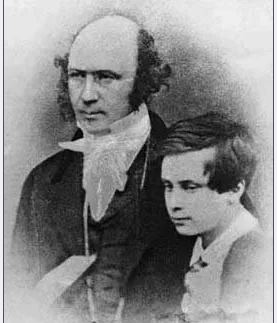
\includegraphics[height=80pt]{hamilton.jpg}
%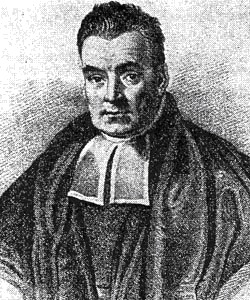
\includegraphics[height=80pt]{bayes.jpg}
%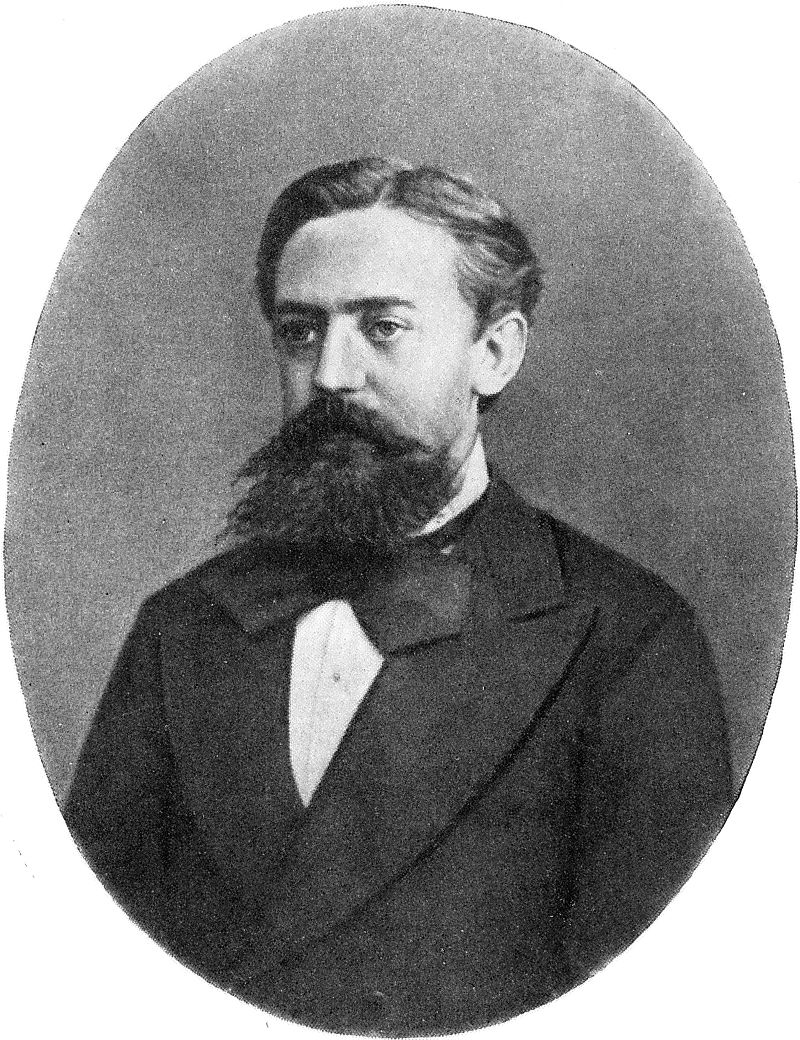
\includegraphics[height=80pt]{markov.jpg}
%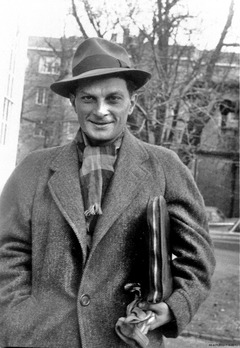
\includegraphics[height=80pt]{ulam.jpg}
%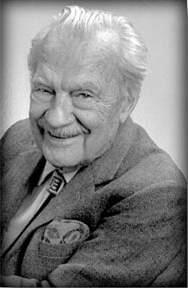
\includegraphics[height=80pt]{metropolis.png}
%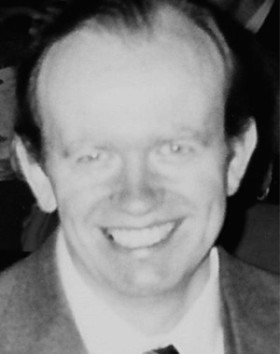
\includegraphics[height=80pt]{hastings.jpg}
%\end{figure}
}
\date{}

\maketitle
\chapter*{Introduction}
%This document contains the lecture notes for the course given at the  MSc. Data Science (2nd year),  Institut Polytechnique de Paris.\footnote{\url{https://www.ip-paris.fr/education/masters/mention-mathematiques-appliquees-statistiques/master-year-2-data-science}} The schedule is roughly the following:
%\begin{enumerate}[$\blacktriangleright$]
%\item Chapter 1-2. Lecture, 1.5H. Tutorial: 2H.
%\item Chapter 2-3. Lecture, 1.5H. Tutorial: 2H.
%\item Chapter 3-4. Lecture, 1.5H. Tutorial: 2H.
%\item Chapter 4-5. Lecture, 1.5H. Tutorial: 2H.
%\item Chapter 5-6. Lecture, 1.5H. Tutorial: 2H.
%\item Chapter 6. Lecture, 1.5H. Tutorial: 2H.
%\end{enumerate}
Numerical illustrations through Jupyter Notebook are given during the course and the source can be run directly in a {\em colaboratory google site} \href{https://colab.research.google.com/drive/1Ey5TNx-_74gPH0FG-rhXSuGGok0T10wS\#}{by following this link}.
%\textcolor{red}{Add github repository with notebooks: independent MH, MALA, HMC.} 
The most curious readers can consult one of these books.
\begin{itemize}
\item {\em Markov Chains and Stochastic Stability} S. Meyn and R. Tweedie. Springer, 2005 (2nd edition).
\item {\em Markov Chains} by R. Douc, E. Moulines, P. Priouret and P. Soulier. Springer, jan. 2019.
\end{itemize}
Interested readers on Monte Carlo techniques can find some inspiration in
\begin{itemize}
\item {\em Monte Carlo Statistical Methods} by G. Casella and C. Robert. Springer, 2004.
\end{itemize}
We thank Kamelia Daudel for her thorough reading and insightful comments.

\clearpage
\newpage

\subsection*{Notation}
The following notations are used throughout these lecture notes.
\begin{itemize}
\item i.i.d.:  independent and identically distributed.
\item r.v.:  random variables.
\item For $r,s \in \nset$ such that $r\leq s$, we write $[r:s]=\{r,r+1,\ldots,s\}$.
\item $X\indep Y$ means that $X$ and $Y$ are independent random variables.
\item $X \eqLaw Y$ means that $X$ and $Y$ have the same law.
\item $\liminf_n a_n=\lim_{n \to\infty} \lr{\inf_{k \geq n} a_k}$ and similarly, $\limsup_n a_n=\lim_{n \to\infty} \lr{\sup_{k \geq n} a_k}$. Moreover, $\lim_n a_n$ exists if and only if $\liminf_n a_n=\limsup_n a_n$.
\item For any $a\in \rset$, $a^+=\max(a,0)$ and $a^-=\max(-a,0)=-\min(a,0)$ and we have $|a|=a^++a^-$ and $a=a^+-a^-$.
\end{itemize}
We also consider the following notions for convergence for random variables.
\begin{enumerate}[$\blacktriangleright$]
\item \fbox{$X_n \weaklim X$} means {\em convergence in distribution} (or "convergence en loi" in French). It is equivalent to any of the following statements.
     \begin{enumerate}[(a)]
     \item For all bounded continuous functions $h$, $\lim_{n}\PE[h(X_n)]=\PE[h(X)]$.
    \item  For all $A \in \borel(\rset)$ such that $\PP(X \in \partial A)=0$,  $\lim_n \PP(X_n \in A)=\PP(X\in A)$.
        \item For all $x\in \rset$ such that $\PP(X=x)=0$, $\lim_n \PP(X_n \leq x)=\PP(X \leq x)$.
\item For all $u \in \rset$, $\lim_n \PE\lrb{\rme^{\rmi u X_n}}=\PE\lrb{\rme^{\rmi u X}}$.
     \end{enumerate}
     In (b), the notation $\partial A$ means the frontier of $A$, that is, the set of points $x$ such that in any neighborhood of $x$, there are an infinite number of distinct points of $A$ and an infinite number of points in $A^c$.
     By abuse of terminology, we may also say that \fbox{\em \bf $X_n$ weakly converges to $X$} instead of stating the distribution of $X_n$ converges weakly to the distribution of $X$.
\item \fbox{$X_n \plim{\PP} X$} means {\em convergence in probability}: for all $\epsilon>0$,
$$
\lim_{n \to \infty} \PP(|X_n -X|>\epsilon)=0.
$$
\item \fbox{$X_n \aslim{\PP} X$} means {\em almost sure convergence}:
$$
\PP(\lim_{n \to \infty}X_n=X)=1\eqsp.
$$
\end{enumerate}
\fbox{Almost sure convergence implies convergence in probability}.
\newcommand{\var}{\mathrm{var}}
The following properties are used many times in these lecture notes.
\begin{enumerate}[(i)]
\item If $X_n \weaklim X$ then for all continuous functions $f$, $f(X_n) \weaklim f(X)$. Note that this property  holds, when $f$ is continuous (and not necessarily bounded), for example $f(u)=u^2$ so that $X_n^2 \weaklim X^2$.
\item \textbf{The Slutsky Lemma.} If $X_n \plim{\PP} c$ where $c$ is a constant and if $Y_n \weaklim Y$, then $(X_n,Y_n) \weaklim (c,Y)$ that is for all continuous functions $f$, $f(X_n,Y_n) \weaklim f(c,Y)$.
\item $X \sim \gauss(0,1)$ if and only if for all $u \geq 0$, $\PE[\rme^{\rmi u
    X}]=\rme^{-u^2/2}$. Moreover, $X \sim \gauss(\mu,\sigma^2)$ if and only if
  for all $u \geq 0$, $\PE[\rme^{\rmi u X}]=\rme^{-u^2 \var{X}/2+\rmi
    u \PE[X]}$ and in that case, $\sigma^2=\var{X}$ and $\mu=\PE(X)$.
 \item Let $c$ be a constant. Then, $X_n \plim{\PP} c$ if and only if $X_n \weaklim c$ (in words, convergence
   in probability to a {\bf constant} is equivalent to convergence in
   distribution to this {\bf constant}).
\end{enumerate}



\dominitoc
\tableofcontents

\chapter{Basics in Markov chains.}
\minitoc
\begin{keywords}
Markov chains, Markov property, Metropolis Hastings, canonical space.
\end{keywords}

%These short lecture notes introduce very basic tools in
%the Markov Chain Monte Carlo (MCMC) theory. We only focus on the
%most fundamental properties that will be useful for a first understanding
%of Metropolis-Hastings (MH) algorithms. Let us start with a gentle and
%smooth introduction to Markov chains.

\section{Main notation}

Let $(\Xset,\Xsigma)$ be a measurable space, i.e.  $\Xsigma$ is a $\sigma$-algebra on $\Xset$, and consider the following notations.
\begin{itemize}
\item $\meas +(\Xset)$ is the set of non-negative measures on $(\Xset,\Xsigma)$.
\item $\meas 1(\Xset)$ is the set of probability measures on $(\Xset,\Xsigma)$.
\item $\funcset{}(\Xset)$ is the set of real-valued measurable functions
$f$ on $\Xset$ and $\funcset{}_{+}(\Xset)$ the set of non-negative measurable
functions on $\Xset$.
\item If $k\leq\ell$,  $u_{k:\ell}$ means $(u_{k},\ldots,u_{\ell})$ and $u_{k:\infty}$ means $(u_{k+\ell})_{\ell\in\nset}$.
\end{itemize}
%Other notation will be introduced progressively.

\section{Definitions}

%We first describe a Markov kernel, which will then be fundamental
%for the definition of a Markov chain. 
\bs
\begin{definition}
We\index{Markov kernel} say that $P:\Xset\times\Xsigma\to\rset^{+}$
is a Markov kernel, if for all $(x,A)\in\Xset\times\Xsigma$,
\begin{itemize}
\item $\Xset\ni y\mapsto P(y,A)$ is $\Xsigma/\mcbb(\rset^{+})$ measurable,
\item $\Xsigma\ni B\mapsto P(x,B)$ is a probability measure on $(\Xset,\Xsigma)$.
\end{itemize}
\end{definition}
\es For all $(x,A)\in\Xset\times\Xsigma$, as a function
of the first component only, $P(\cdot,A)$ is measurable and as a
function of the second component only, $P(x,\cdot)$ is a probability
measure. In particular, $P(x,\Xset)=1$ for all $x\in\Xset$. Since
$P(x,\cdot)$ is a measure, we also use the infinitesimal notation:
$P(x,\rmd y)$. For example, 
$$
P(x,A)=\int_{\Xset}\indi A(y)P(x,\rmd y)=\int_{A}P(x,\rmd y)\eqsp.
$$
In almost all the course, a Markov kernel $P$ allows to move a point $x$ from a measurable space $(\Xset,\Xsigma)$ to another point on the same measurable space, that is, $P$ is defined on $\Xset\times \Xsigma$ but we can more generally define a Markov kernel from a measurable space $(\Xset,\Xsigma)$ to another measurable space $(\Yset,\Ysigma)$. In such case, $P$ will be a  Markov kernel on $\Xset \times \Ysigma$. 
\begin{definition}
\label{def:MarkovChain} Let\index{Markov chain} $\seq{X_{k}}{k\in\nset}$
be a sequence of random variables on the same probability space $(\Omega,\mcg,\PP)$
and taking values on $\Xset$, we say that $\seq{X_{k}}{k\in\nset}$
is a Markov chain with Markov kernel $P$ and initial distribution
$\nu\in\meas 1(\Xset)$ if and only if
\begin{enumerate}[(i)]
\item  for all $(k,A)\in\nset\times\Xsigma$,  $\PP(X_{k+1}\in A|X_{0:k})=P(X_{k},A)$,
$\PP$-a.s.
\item $\PP(X_{0}\in A)=\nu(A)$.
\end{enumerate}
\end{definition}
Note that in the definition we consider $\PP(X_{k+1}\in A|X_{0:k})$,
that is, the conditional probability is with respect to the sigma-field
$\sigma(X_{0:k})$. We can actually replace $\sigma(X_{0:k})$ by
$\mcf_{k}$ as soon as we know that $(X_{k})_{k\geq0}$ is $(\mcf_{k})_{k\geq0}$-adapted.

If $\seq{\mcf_{k}}{k\in\nset}$
is a sequence of embedded sigma-fields on $\Xset$ (that is, $\mcf_{k}\subset\mcf_{k+1}$
for all $k\in\nset$), then $\seq{\mcf_{k}}{k\in\nset}$ is called a \textbf{filtration} \index{filtration}
on $\Xset$ and we say that $(X_{k})_{k\geq0}$ is $(\mcf_{k})_{k\geq0}$-adapted
if $X_{k}$ is $\mcg/\mcf_{k}$-measurable for all $k\in\nset$. Of
course, the most natural filtration for $\seq{X_{k}}{k\in\nset}$
is indeed $\mcf_{k}=\sigma(X_{0:k})$ and unsurprisingly, we call
it the \textbf{natural filtration}\index{filtration!natural}. But other possibilities exist,
where $\mcf_{k}$ is enlarged to include some other variables alongside
with $X_{0:k}$. For example, let $\seq{Y_{k}}{k\in\nset}$ be any
other sequence of random variables on $(\Omega,\mcg,\PP)$ and taking
values in $\Xset$ (we do not assume anything on the relation between  $\seq{X_{k}}{k\in\nset}$ and $\seq{Y_{k}}{k\in\nset}$). A typical example corresponds
to $X_{k+1}=g(X_{0:k},Y_{0:k})$, but we do not even need to assume
that for the moment. Set $\mcf_{k}=\sigma(X_{0:k},Y_{0:k})$ and assume
that
\begin{equation}
\PP(X_{k+1}\in A|\mcf_{k})=P(X_{k},A),\quad\as\label{eq:def:MC:F-k}
\end{equation}
Since $X_{\ell}$ is $\mcf_{\ell}$-measurable and $\mcf_{\ell}\subset\mcf_{k}$
for $\ell\leq k$, we deduce that $\sigma(X_{0:k})\subset\mcf_{k}$.
This allows to apply the tower property, which yields
\begin{align*}
\PP(X_{k+1}\in A|X_{0:k}) & =\PE\lrb{\PP(X_{k+1}\in A|\mcf_{k})|X_{0:k}}\\
 & =\PE\lrb{P(X_{k},A)|X_{0:k}}=P(X_{k},A),\quad\as
\end{align*}
and therefore if we assume \Eqref{def:MC:F-k}, then as soon as $(X_{k})_{k\geq0}$
is $(\mcf_{k})_{k\geq0}$-adapted, we can conclude that $\seq{X_{k}}{k\in\nset}$
is a Markov chain with Markov kernel $P$. Why is it useful? Well,
Sometimes, we define iteratively $X_{k+1}$ using other variables
rather than $X_{0:k}$ only and therefore, considering $\PP(X_{k+1}\in A|\mcf_{k})$
is easier to deal with. Let us see it in action with a very simple
example.
\begin{example}
Let $\seq{\epsilon_{k}}{k\geq1}$ be i.i.d. random variables on $\rset^{p}$
with density $f$ with respect to the Lebesgue measure on $\rset^{p}$,
and let $X_{0}\sim\mu$. We assume that $X_{0}$ is independent of
$\seq{\epsilon_{k}}{k\in\nset}$. Define
\[
X_{k+1}=aX_{k}+b\epsilon_{k+1}\,,\quad k\in\nset.
\]
Set $\mcf_{0}=\sigma(X_{0})$ and for $k\geq1$, $\mcf_{k}=\sigma(X_{0},\epsilon_{1:k})$.
Since $X_{\ell}$ is a deterministic function of $X_{0}$ and $\epsilon_{1:\ell}$,
we deduce that $(X_{k})_{k\geq0}$ is $(\mcf_{k})_{k\geq0}$-adapted.
Therefore, we only need to check \Eqref{def:MC:F-k}. Now, for any
non-negative or bounded measurable function $h$ on $\Xset$, 
\[
\PE[h(X_{k+1})|\mcf_{k}]=\int_{-\infty}^{\infty}h(\underbrace{aX_{k}+b\epsilon}_{y})f(\epsilon)\rmd\epsilon=\int_{-\infty}^{\infty}h(y)\underbrace{f\lr{\frac{y-aX_{k}}{b}}\frac{1}{b^{p}}\rmd y}_{P(X_{k},\rmd y)},
\]
where the last equality follows from an adequate change of variable.
Therefore, $\seq{X_{k}}{k\in\nset}$ is a Markov chain with Markov
kernel
\[
(x,A)\mapsto P(x,A)=\int_{A}f\lr{\frac{y-ax}{b}}\frac{1}{b^{p}}\rmd y.
\]
In this example, we can check that $\mcf_{k}$ is actually the natural
filtration of $\seq{X_{k}}{k\in\nset}$ but we even do not need to
check this property for getting that $\seq{X_{k}}{k\in\nset}$ is
a Markov chain.
\end{example}
\blb\textbf{ Key notions. } At this stage, we know how 
to solve typical exercises where some random variables are given and
the question is to determine whether these random variables form a
Markov chain or not and if yes, what is the expression of the associated
Markov kernel. \elb
As an illustration, interested readers might try to solve Exercise~\ref{ex:arch}.


\subsection{Additional notation}
For all $\mu\in\meas +(\Xset)$, all Markov kernels $P$, $Q$ on
$\Xset\times\Xsigma$, and all measurable non-negative or bounded
functions on $h$ on $\Xset$, we use the following convention and
notation.
\begin{itemize}
\item $\mu P$ is the (positive) measure: $\Xsigma\ni A\mapsto\mu P(A)=\int\mu(\rmd x)P(x,A)$,
\item $PQ$ is the Markov kernel: $(x,A)\mapsto\int_{\Xset}P(x,\rmd y)Q(y,A)$,
\item $Ph$ is the measurable function $x\mapsto\int_{\Xset}P(x,\rmd y)h(y)$.
\end{itemize}
It is easy to check that if $\mu$ is a probability measure, then
$\mu P$ is also a probability measure (since $\mu P(\Xset)=\int_{\Xset}\mu(\rmd x)P(x,\Xset)=\int_{\Xset}\mu(\rmd x)=1$).
With this notation, using Fubini's theorem,
\begin{align*}
\mu(P(Qh)) & =(\mu P)(Qh)=(\mu(PQ))h\\
 & =\mu((PQ)h)=\int_{\Xset^{3}}\mu(\rmd x)P(x,\rmd y)Q(y,\rmd z)h(z).
\end{align*}
Therefore, all these parenthesis can be discarded and we can write
$\mu PQh$ without any ambiguity. 
To sum up, measures act on the left side of a Markov kernel whereas
functions acts on the right side. To make sure you have mastered all
the notation, check your understanding with the following equalities
$\delta_{x}P(A)=P(x,A)=P\indi A(x)$.

To finish up with notation, we now define the iterates of a Markov
kernel $P$, which will come in very handy thereafter: for a given
Markov kernel $P$ on $\Xset\times\Xsigma$, define $P^{0}=I$ where
$I$ is the identity kernel: $(x,A)\mapsto\indi A(x)$, and set for
$k\geq0$, $P^{k+1}=P^{k}P$.

\bfr
\begin{lemma}
Let $\seq{X_{k}}{k\in\nset}$ be a Markov chain on the same probability
space $(\Omega,\mcg,\PP)$ and taking values on $\Xset$, with Markov
kernel $P$ and with initial distribution $\nu\in\meas 1(\Xset)$.
Then, for any $n\in\nset$, the law of $X_{0:n}$ is $\nu(\rmd x_{0})\prod_{i=0}^{n-1}P(x_{i},\rmd x_{i+1})$
(with the convention that $\prod_{i=0}^{-1}=1$).
\end{lemma}
\efr
\begin{svmultproof}
Recall that for all $(n,A)\in\nset\times\Xsigma$, $\PP(X_{n+1}\in A|X_{0:n})=P(X_{n},A)$,
$\PP$-a.s. or equivalently for all non-negative measurable functions
$h_{n+1}$ on $\Xset$, $\PE\left[h_{n+1}(X_{n+1})|X_{0:n}\right]=Ph_{n+1}(X_{n})$ $\PP$-a.s.
We now show by induction that for all $n\in\nset$,
\begin{center}
$(H_{n})$ the law of $X_{0:n}$ is $\nu(\rmd x_{0})\prod_{i=0}^{n-1}P(x_{i},\rmd x_{i+1})$.
\par\end{center}
We first note that $(H_{0})$ is true since by assumption, $X_{0}\sim\nu$.
Assume now that $(H_{n})$ holds for some $n\in\nset$. Then, for
all non-negative measurable functions $h_{0},\ldots,h_{n+1}$ on $\Xset$,
the tower property yields

\[
\PE\left[\prod_{i=0}^{n+1}h_{i}(X_{i})\right]=\PE\left[\left(\prod_{i=0}^{n}h_{i}(X_{i})\right)\ \PE\left[h_{n+1}(X_{n+1})|X_{0:n}\right]\right]=\PE\left[\left(\prod_{i=0}^{n}h_{i}(X_{i})\right)\ Ph_{n+1}(X_{n})\right],
\]
 and since the inner term in the rhs only depends on $X_{0:n}$, we
can apply $(H_{n})$ and thus,
\begin{align*}
\PE\left[\prod_{i=0}^{n+1}h_{i}(X_{i})\right] & =\int_{\Xset^{n+1}}\left[\nu(\rmd x_{0})\prod_{i=0}^{n-1}P(x_{i},\rmd x_{i+1})\right]\left(\prod_{i=0}^{n}h_{i}(x_{i})\right)\ Ph_{n+1}(x_{n})\\
 & =\int_{\Xset^{n+1}}\left[\nu(\rmd x_{0})\prod_{i=0}^{n}P(x_{i},\rmd x_{i+1})\right]\left(\prod_{i=0}^{n+1}h_{i}(x_{i})\right),
\end{align*}
which shows that the law of $X_{0:n+1}$ is $\nu(\rmd x_{0})\prod_{i=0}^{n}P(x_{i},\rmd x_{i+1})$
and $\left(H_{n+1}\right)$ is thus proved.
\end{svmultproof}
As a consequence, the marginal law of $X_{n}$ is given by integrating
$\nu(\rmd x_{0})\prod_{i=0}^{n-1}P(x_{i},\rmd x_{i+1})$ over $x_{0:n-1}$
and thus, for all $A\in\Xsigma$,
\[
\PP(X_{n}\in A)=\int_{\Xset^{n+1}}\indi A(X_{n})\nu(\rmd x_{0})\prod_{i=0}^{n-1}P(x_{i},\rmd x_{i+1})=\nu P^{n}(A),
\]
 that is, $\nu P^{n}$ is the distribution of $X_{n}$ or in a compact
notation, $\boxed{X_{n}\sim\nu P^{n}}$.

\section{Canonical space} \index{canonical space}

In the previous sections, the $\seq{X_{k}}{k\in\nset}$
are already given and we check the two items in the definition of
a Markov chain (\Defref{MarkovChain}) with Markov kernel $P$ and initial
distribution $\nu$. We now turn to the reverse situation where a
couple $(\nu,P)$  of initial distribution and Markov kernel are given
beforehand and we intend to construct the random variables $\seq{X_{k}}{k\in\nset}$
on some convenient (common) probability space $(\Omega,\mcf,\PP)$
such that $\seq{X_{k}}{k\in\nset}$ is a Markov chain with Markov
kernel $P$ and initial distribution $\nu$.

\subsection{A simpler problem }

We start with an easier problem where we only want to construct $\seq{X_{k}}{k\in[0:n-1]}$
where $n$ is some given positive integer. That is, we only consider
\textbf{a finite range of integers} such that the first item in \defref{MarkovChain}
is satisfied. For a given $\nu\in\meas 1(\Xset)$, define the triplet
$(\Omega_{n},\mcg_{n},\PP_{\nu,n})$ as follows:
\begin{itemize}
\item $\Omega_{n}=\Xset^{n+1}$, $\mcg_{n}=\Xsigma^{\otimes(n+1)}$ and
$\PP_{\nu,n}$ is the probability measure defined on $(\Omega_{n},\mcg_{n})$
by
\[
\mcg_{n}\ni A\mapsto\PP_{\nu,n}(A)=\int_{\Xset^{n+1}}\indi A(\omega_{0:n})\nu(\rmd\omega_{0})\prod_{i=1}^{n}P(\omega_{i-1},\rmd\omega_{i}),
\]
\end{itemize}
and for $\omega\in\Omega_{n}$, set $X_{k}(\omega)=\omega_{k}$, i.e.
$X_{k}(\omega)$ is the projection of the k-th component of $\omega$.

We aim to show that for all $A\in\Xsigma$ and all $k\in[0:n-1]$,
we have $\PP_{\nu,n}(X_{k+1}\in A|X_{0:k-1})=P(X_{k},A),\;\PP_{\nu,n}-a.s.$
To do so, write for any $k\in[0:n-1]$, any non-negative measurable
function $h$ on $\Xset^{k+1}$ and any $A\in\Xsigma$
\begin{align*}
\PE_{\nu,n}\lrb{h(X_{0:k})\indi A(X_{k+1})} & =\int_{\Xset^{k+2}}h(\omega_{0:k})\indi A(\omega_{k+1})\nu(\rmd\omega_{0})\prod_{i=1}^{k+1}P(\omega_{i-1},\rmd\omega_{i})\\
 & =\int_{\Xset^{k+2}}h(\omega_{0:k})P(\omega_{k},A)\nu(\rmd\omega_{0})\prod_{i=1}^{k}P(\omega_{i-1},\rmd\omega_{i})\\
 & =\PE_{\nu,n}\lrb{h(X_{0:k})P(X_{k},A)}.
\end{align*}
Since h is arbitrary, this is equivalent to saying that $\PP_{\nu,n}(X_{k+1}\in A|X_{0:k})=P(X_{k},A)\,,\quad\PP-a.s.$

\subsection{The general case }

We now consider the general case where $k\in\nset$ instead of $k\in[0:n-1]$.
Define the coordinate process $(X_{n})_{n\geq 0}$ by $X_{n}(\omega)=\omega_{n}$
for all $\omega\in\Xset^{\nset}$. We will sometimes use $X_{k:\ell}:\omega\mapsto(\omega_{k},\ldots,\omega_{\ell})$
for $k\leq\ell$ and by extension $X_{k:\infty}:\omega\mapsto(\omega_{k},\ldots,\omega_{\ell},\omega_{\ell+1},\dots)$.
In particular, $X_{0:\infty}(\omega)=\mathrm{Id}(\omega)=\omega$ where $\mathrm{Id}$
is the identity function.

\bs
\begin{theorem}
\label{th:canonical}
\textbf{(The canonical space)}\index{canonical space} Let $(\Xset,\Xsigma)$ be a measurable
space and let $P$ be a Markov kernel on $\Xset\times\Xsigma$. For
every probability measure $\nu\in\meas 1(\Xset)$, there exists a
unique probability measure $\PP_{\nu}$ on the canonical space $(\Xset^{\nset},\Xsigma^{\otimes\nset})$
such that, under $\PP_{\nu}$, the coordinate process $\seq{X_{n}}{n\in\nset}$
is a Markov chain with Markov kernel $P$ and initial distribution
$\nu$.
\end{theorem}
\es This result is often referred to as the \emph{Ionescu-Tulcea
theorem}. Its proof goes far beyond the scope of this course and we
will admit it here. Some other, much simpler proofs exist and are
based on the Kolmogorov extension theorem, but they hold at the price
of additive assumptions on the space (in contrast, we only assume
here that $(\Xset,\Xsigma)$ is a measurable space, which is quite
minimal). In the canonical representation, we therefore set $\Omega=\Xset^{\nset}$,
$\mcg=\Xsigma^{\otimes\nset}$ and $\PP=\PP_{\nu}$. In the particular
case where the initial distribution $\nu$ is a Dirac mass, we use
the compact notation $\boxed{\PP_{x}=\PP_{\delta_{x}}}$. Thus, Theorem~\ref{th:canonical} allows to define not only one probability measure but a family
of probability measures $(\PP_{\nu})_{\nu\in\meas 1(\Xset)}$ on the
space of trajectories.

\textbf{What are the relations between the probability measures $(\PP_{\nu})_{\nu\in\meas 1(\Xset)}$?}
A consequence of this theorem is that for all $A\in\Xsigma^{\otimes(n+1)}$,
$\PP_{\nu}(X_{0:n}\in A)=\int_{A}\nu(\rmd\omega_{0})\prod_{i=1}^{n}P(\omega_{i-1},\rmd\omega_{i})$.
Replacing $\nu$ by $\delta_{x_{0}}$ and comparing the two obtained
expressions, we get
\[
\PP_{\nu}(X_{0:n}\in A)=\int_{\Xset}\nu(\rmd x_{0})\PP_{x_{0}}(X_{0:n}\in A).
\]
We can actually extend this result to any $A\in\Xsigma^{\otimes\nset}$
by replacing the $n+1$ -tuple $X_{0:n}$ by the (infinite) trajectory
$X_{0:\infty}$. First note the following equalities: $A=\left\{ \omega\in A\right\} =\set{\omega\in\Omega}{X_{0:\infty}(\omega)\in A}=\left\{ X_{0:\infty}\in A\right\} $.
\begin{framed}
We then obtain the following identity: for all $A\in\Xsigma^{\otimes\nset}$,

\begin{equation}
\PP_{\nu}(A)=\PP_{\nu}(X_{0:\infty}\in A)=\int_{\Xset}\nu(\rmd x_{0})\PP_{x_{0}}(X_{0:\infty}\in A)=\int_{\Xset}\nu(\rmd x_{0})\PP_{x_{0}}(A).\label{eq:relation:P}
\end{equation}

\end{framed}

An illustration is given in Exercise~\ref{exo:solidarite}.
\subsection{The Markov property.} \index{Markov property}

Define the shift operator $S$ by $S:\Xset^{\nset}\ni\omega\mapsto\omega'\in\Xset^{\nset}$
where $\omega=(\omega_{i})_{i\in\nset}$ and $\omega'=(\omega_{i+1})_{i\in\nset}$.

\bs
\begin{theorem}
\textbf{(The Markov property)} For any $\nu\in\meas 1(\Xset)$, any
non-negative or bounded function $h$ on $\Xset^{\nset}$ and any
$n\in\nset$,
\begin{equation}
\PE_{\nu}\left[h\circ S^{k}|\mcf_{k}\right]=\PE_{X_{k}}[h]\,,\quad\PP_{\nu}-a.s.\label{eq:MarkovProperty}
\end{equation}
where $\mathcal{F}_{k}=\sigma(X_{0:k})$.
\end{theorem}
\es

By definition of $X_{k:\infty}$, we have $\PP_{\nu}-a.s.$,
\begin{align*}
\PE_{\nu}\left[h(X_{k:\infty})|\mcf_{k}\right] & =\PE_{\nu}\left[h\circ S^{k}\circ X_{0:\infty}|\mcf_{k}\right]=\PE_{\nu}\left[h\circ S^{k}\circ \mathrm{Id}|\mcf_{k}\right]\\
 & =\PE_{\nu}\left[h\circ S^{k}|\mcf_{k}\right]=\PE_{X_{k}}[h]=\PE_{X_{k}}[h\circ \mathrm{Id}]\\
 & =\PE_{X_{k}}[h(X_{0:\infty})].
\end{align*}
 Therefore, for any $\nu\in\meas 1(\Xset)$,
\[
\boxed{\PE_{\nu}\left[h(X_{k:\infty})|\mcf_{k}\right]=\PE_{X_{k}}[h(X_{0:\infty})]\,,\quad\PP_{\nu}-a.s.}
\]
 is another \textbf{equivalent expression of the Markov property.
}This expression may seem easier to deal with but the reader has to
be at ease with both formulations. A stronger version of the Markov
property exists and is called (as expected) the strong Markov property:
its statement is \Eqref{MarkovProperty} with the exception that $k$
is replaced by a stopping time $\tau$ and that the identity only
holds on the event $\left\{ \tau<\infty\right\} $. The strong Markov
property is extremely important in Markov Chain theory but, quite
surprisingly, it is not needed in this course.  Exercise~\ref{exo:strongMarkov} states and proves the Strong Markov property.


\section{Key notions of this chapter}
\begin{center}
\shadowbox{\begin{minipage}{0.9\textwidth}
\begin{enumerate}[a)]
\item Writing expressions of Markov kernels.
\item Understand the different notations $\mu P$,  $Q f$...
\item Understanding the canonical space.
\item Understanding \eqref{eq:relation:P}.
\item Making use of the Markov property \eqref{eq:MarkovProperty}.
\end{enumerate}
\end{minipage}
}
\end{center}



\begin{subappendices}
\section*{Highlights}

\section{Andrey Markov (source: wikipedia).}

\begin{wrapfigure}{L}{0.25\textwidth} \centering

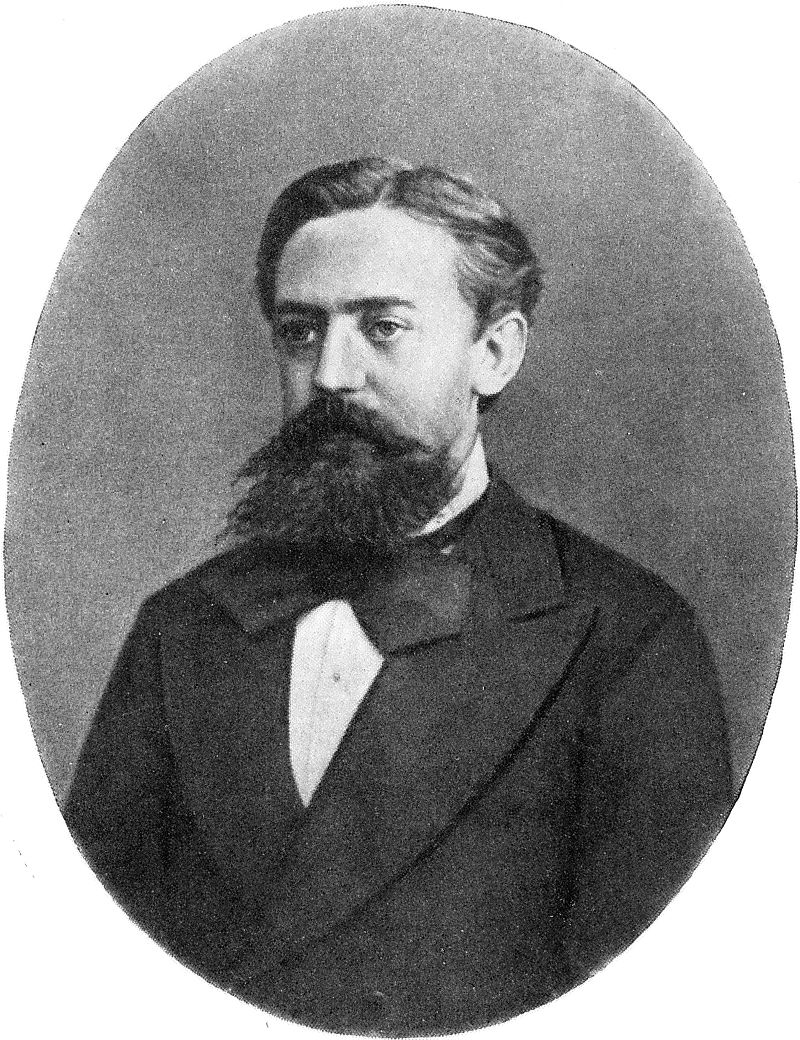
\includegraphics[scale=0.1]{markov}

\end{wrapfigure}Andrey Andreyevich Markov (1856--1922) was a Russian
mathematician best known for his work on stochastic processes. A primary
subject of his research later became known as Markov chains and Markov
processes.

Markov and his younger brother Vladimir Andreevich Markov (1871--1897)
proved the Markov brothers' inequality. His son, another Andrei Andreyevich
Markov (1903--1979), was also a notable mathematician, making contributions
to constructive mathematics and recursive function theory.

Andrey Markov was born on 14 June 1856 in Russia. He attended Petersburg
Grammar, where he was seen as a rebellious student by a select few
teachers. In his academics he performed poorly in most subjects other
than mathematics. Later in life he attended Petersburg University;
among his teachers were Yulian Sokhotski (differential calculus, higher
algebra), Konstantin Posse (analytic geometry), Yegor Zolotarev (integral
calculus), Pafnuty Chebyshev (number theory and probability theory),
Aleksandr Korkin (ordinary and partial differential equations), Mikhail
Okatov (mechanism theory), Osip Somov (mechanics), and Nikolai Budaev
(descriptive and higher geometry). He completed his studies at the
University and was later asked if he would like to stay and have a
career as a Mathematician. He later taught at high schools and continued
his own mathematical studies. In this time he found a practical use
for his mathematical skills. He figured out that he could use chains
to model the alliteration of vowels and consonants in Russian literature.
He also contributed to many other mathematical aspects in his time.
He died at age 66 on 20 July 1922.

\end{subappendices}

\chapter{Invariant probability measures}
\minitoc
\begin{keywords}
Invariant probability measures, existence, uniqueness, reversibility.
\end{keywords}
\section{Invariant probability measures: existence}
\index{invariant!probability measure}
\begin{framed}%
\begin{definition}
We say that $\pi\in\meas 1(\Xset)$ is an invariant probability measure
for the Markov kernel $P$ on $\Xset\times\Xsigma$ if $\pi P=\pi$.
\end{definition}
\end{framed}

If $(X_{k})$ is a Markov chain with Markov kernel $P$
and assuming that $X_{0}\sim\pi$, then for all $k\geq1$, we have
$X_{k}\sim\pi$ since applying $P^{k}$ on
both sides of $\pi P=\pi$ shows that $\pi P^{k+1}=\pi P^{k}$ and
therefore, for all $k\in\nset$, $\pi P^{k}=\pi$. This result on
the (marginal) distribution of $X_{k}$ may be extended to $n$-tuples.

More precisely, it can be readily checked that if $\pi$ is an \emph{invariant
probability measure }for $P$, then the sequence of random variables
$\seq{X_{k}}{k\in\nset}$ is a \emph{strongly stationary sequence}
under $\PP_{\pi}$ (in the sense that for all $n,p\in\nset^{*}$,
and all n-tuple $k_{1:n}$, the random vector $(X_{k_{1}},\ldots,X_{k_{n}})$
follows the same distribution as $(X_{k_{1}+p},\ldots,X_{k_{n}+p}))$.

Exercises~\ref{exo:invar:one} and \ref{exo:invar:two} illustrate the existence of stationary distributions for Markov chains.
We now introduce the notion of reversibility for a Markov kernel.
This will be of crucial importance for designing Markov kernels with
a given invariant probability measure.

\bs
\begin{definition}
Let $\pi\in\meas 1(\Xset)$ and $P$ be a Markov kernel on $\Xset\times\Xsigma$.
We say that $P$ is $\pi$-reversible if and only if (with infinitesimal
notation)

\index{reversibility}
\begin{equation}
\pi(\rmd x)P(x,\rmd y)=\pi(\rmd y)P(y,\rmd x),\label{eq:reversibility}
\end{equation}
that is, for all measurable bounded or non-negative functions $h$
on $\left(\Xset^{2},\Xsigma^{\otimes2}\right)$,
\begin{equation}
\iint_{\Xset^{2}}h(x,y)\pi(\rmd x)P(x,\rmd y)=\iint_{\Xset^{2}}h(x,y)\pi(\rmd y)P(y,\rmd x).\label{eq:reversibility:h}
\end{equation}
\end{definition}
\es A Markov kernel $P$ is $\pi$-reversible if and only
if the probability measure $\pi(\rmd x)P(x,\rmd y)$ is symmetric
with respect to $(x,y)$. \bs
\begin{proposition}
Let $P$ be a Markov kernel on $\Xset\times\Xsigma$. Let $\pi\in\meas 1(\Xset)$
such that $P$ is $\pi$-reversible, then the Markov kernel $P$ is
$\pi$-invariant.
\end{proposition}
\es
\begin{svmultproof}
For any $A\in\Xsigma$, we have by the reversibility relation

\[
\pi P(A)=\iint_{\Xset^{2}}\indi A(y)\pi(\rmd x)P(x,\rmd y)=\iint_{\Xset^{2}}\indi A(y)\pi(\rmd y)P(y,\rmd x)=\int_{A}\pi(\rmd y)\underbrace{P(y,\Xset)}_{1}=\pi(A),
\]

which finishes the proof.
\end{svmultproof}

\begin{leftbar}

\textbf{What are the consequences?} If you want to check easily that
a kernel $P$ is $\pi$-invariant, it is sufficient to check that
it is $\pi$-reversible.

\end{leftbar}

Exercise~\ref{exo:gibbs} gives an example of $\pi$-reversible kernel.

\subsection{Metropolis-Hastings (MH) algorithms}
\label{sec:MH}
\index{Metropolis Hastings}
In this section, we are given a probability measure $\pi\in\meas 1(\Xset)$
and the idea now is to construct a Markov chain $\seq{X_{k}}{k\in\nset}$
admitting $\pi$ as invariant probability measure, in which case we
say that $\pi$ is a target distribution. In other words, we try to
find a Markov kernel $P$ on $\Xset\times\Xsigma$ such that $P$
is $\pi$-invariant. The reason for that is that an invariant probability
measure will be a good candidate for the ``limiting'' distribution
of $\seq{X_{k}}{k\in\nset}$ (in some sense to be defined) and this
in turn, will allow us to provide an approximation $\pi(h)$:
\[
\pi(h)=\int_{\Xset}h(x)\pi(\rmd x)\approx n^{-1}\sum_{k=0}^{n-1}h(X_{i}).
\]


\subsubsection{Construction of the kernel\label{subsec:construc}}

For simplicity we now assume that $\pi$ has a density with respect
to some dominating $\sigma$-finite measure $\lambda$ and by abuse
of notation, we also denote by $\pi$ this density, that is we write
$\pi(\rmd x)=\pi(x)\lambda(\rmd x)$ and we assume that this density
$\pi$ is \textbf{positive}.

Moreover, let $Q$ be Markov kernel on $\Xset\times\Xsigma$ such
that $Q(x,\rmd y)=q(x,y)\lambda(\rmd y)$, that is, for any $x\in\Xset$,
$Q(x,\cdot)$ is also dominated by $\lambda$ and denoting by $q(x,\cdot)$
this density, we assume for simplicity that $q(x,y)$ is \textbf{positive}
for all $x,y\in\Xset$. At this stage, there is almost no link between
$Q$ and the target distribution $\pi$.

For a given function $\alpha:\Xset^{2}\to[0,1]$, consider the following Algorithm~\ref{alg:mh}.

\begin{algorithm}
\caption{\label{alg:mh}The Metropolis Algorithm}

%\SetAlgoLined
\SetKwInOut{Input}{input}\SetKwInOut{Output}{output}
\Input{n}
\Output{$X_0,\ldots,X_n$}
\BlankLine
At $t=0$, draw $X_{0}$ according to some arbitrary distribution\\
\For{$t\leftarrow 0$ \KwTo $n-1$}
{
$\bullet$ Draw independently $Y_{t+1}\sim Q(X_{t},\cdot)$ and $U_{t+1}\sim\mathrm{Unif}(0,1)$\\
$\bullet$ Set $X_{t+1}=\begin{cases} Y_{t+1} & \mbox{if }U_{t+1}\leq\alpha(X_{t},Y_{t+1})\\ X_{t} & \mbox{otherwise} \end{cases}$
}
\end{algorithm}
 In words, $Q$ allows to propose a candidate for the next value of
the Markov chain $(X_{k})$ and this candidate will be accepted or
refused according to a probability that depends on the function $\alpha$.

We will now choose conveniently $\alpha$ in such a way that $(X_{k})$
is a Markov chain with invariant probability measure $\pi$. The concept
of $\pi$-reversibility will help us. To do so, let us assume that
for all $x,y\in\Xset$,

\begin{equation}
\pi(x)\alpha(x,y)q(x,y)=\pi(y)\alpha(y,x)q(y,x),\label{eq:balance}
\end{equation}
and let us show that it implies that the Markov kernel P associated
to $(X_{k})$ is $\pi$-reversible.

First, we write down the Markov kernel associated to $(X_{k})$: in
passing, this is an excellent opportunity to check if we are able
to express explicitly a Markov kernel by analyzing conveniently the
update transition. Denote $\mcf_{t}=\sigma(X_{0},U_{1:t},Y_{1:t})$
and note that $(X_{t})$ is adapted to the filtration $(\mcf_{t})$
(which is equivalent to $\sigma(X_{0,t})\subset\mcf_{t}$). Then,
setting $\bar{\alpha}(x)=1-\int_{\Xset}Q(x,\rmd y)\alpha(x,y)$, we
have for any bounded or non-negative measurable function $h$ on $\Xset$
and any $t\in\nset$,

\begin{align*}
\PE\lrb{h(X_{t+1})|\mcf_{t}} & =\PE\lrb{\indiacc{U_{t+1}<\alpha(X_{t},Y_{t+1})}h(Y_{t+1})|\mcf_{t}}+\PE\lrb{\indiacc{U_{t+1}\geq\alpha(X_{t},Y_{t+1})}|\mcf_{t}}h(X_{t})\\
 & =\int_{\Xset}Q(X_{t},\rmd y)\alpha(X_{t},y)h(y)+\bar{\alpha}(X_{t})h(X_{t})\\
 & =\int_{\Xset}\lrb{\underbrace{Q(X_{t},\rmd y)\alpha(X_{t},y)+\bar{\alpha}(X_{t})\delta_{X_{t}}(\rmd y)}_{\mh{\pi,Q}(X_{t},\rmd y)}}h(y)=\mh{\pi,Q}h(X_{t}).
\end{align*}
Therefore, $\seq{X_{t}}{t\in\nset}$ is a Markov chain with Markov
kernel
\begin{equation}
\mh{\pi,Q}(x,\rmd y)=Q(x,\rmd y)\alpha(x,y)+\bar{\alpha}(x)\delta_{x}(\rmd y).\label{eq:def:mh}
\end{equation}
 \bs
\begin{lemma}
\label{lem:reversible} The Markov kernel $\mh{\pi,Q}$ is $\pi$-reversible
if and only if

\begin{equation}
\pi(\rmd x)Q(x,\rmd y)\alpha(x,y)=\pi(\rmd y)Q(y,\rmd x)\alpha(y,x).\label{eq:balance:detaillee}
\end{equation}
\end{lemma}
\es In this literature, \Eqref{balance:detaillee} is often called
the \textbf{detailed balance condition.}
\begin{svmultproof}
First, note that
\begin{equation}
\pi(\rmd x)\bar{\alpha}(x)\delta_{x}(\rmd y)=\pi(\rmd y)\bar{\alpha}(y)\delta_{y}(\rmd x).\label{eq:balance:dirac}
\end{equation}
Indeed, for any measurable function $h$ on $\Xset^{2}$, we have

\begin{align*}
\iint_{\Xset^{2}}h(x,y)\pi(\rmd x)\bar{\alpha}(x)\delta_{x}\lr{\rmd y} & =\int_{\Xset}h(x,x)\pi(\rmd x)\bar{\alpha}(x)\\
 & =\int_{\Xset}h(y,y)\pi(\rmd y)\bar{\alpha}(y)=\iint_{\Xset^{2}}h(x,y)\pi(\rmd y)\bar{\alpha}(y)\delta_{y}(\rmd x).
\end{align*}

Combining \Eqref{def:mh} with \Eqref{balance:dirac}, we obtain that
$\mh{\pi,Q}$ is $\pi$-reversible if and only if the detailed balance
condition \Eqref{balance:detaillee} is satisfied. This completes
the proof.
\end{svmultproof}


\subsubsection{Acceptance probability}
\index{Acceptance probability}
We now make use of \Lemref{reversible} in order to find an explicit
expression of the acceptance probability $\alpha$. We have the following
lemma.

\bfr
\begin{lemma}
\label{lem:acceptance} Denote $\alpha^{MH}(x,y)=\min\lr{\frac{\pi(y)q(y,x)}{\pi(x)q(x,y)},1}$
and $\alpha^{b}(x,y)=\frac{\pi(y)q(y,x)}{\pi(x)q(x,y)+\pi(y)q(y,x)}$.
Then, any $\alpha\in\left\{ \alpha^{MH},\alpha^{b}\right\} $ satisfies
the detailed balance condition \eqref{eq:balance:detaillee}. Moreover, any other $\alpha\in[0,1]$
that satisfies the detailed balance condition is dominated by $\alpha^{MH}$in
the sense that: for $\lambda^{\otimes2}$-almost all $x,y\in\Xset$,
\begin{equation}
\alpha(x,y)\leq\alpha^{MH}(x,y).\label{eq:accept:max}
\end{equation}

\end{lemma}
\efr
\begin{svmultproof}
The fact that any $\alpha\in\left\{ \alpha^{MH},\alpha^{b}\right\} $
satisfies $\pi(x)q(x,y)\alpha(x,y)=\pi(y)q(y,x)\alpha(y,x)$ for $\lambda^{\otimes2}$-almost
all $x,y\in\Xset$, is immediate, by replacing $\alpha$ by its expression.
It remains to check \Eqref{accept:max} . Assume now that for $\lambda^{\otimes2}$-almost
all $x,y\in\Xset$,
\[
\pi(x)q(x,y)\alpha(x,y)=\pi(y)q(y,x)\alpha(y,x).
\]
then, using that $\alpha(y,x)\leq1$ shows that $\alpha(x,y)\leq\frac{\pi(y)q(y,x)}{\pi(x)q(x,y)}$.
Moreover, $\alpha(x,y)\leq1$ and this finally implies
\[
\alpha(x,y)\leq\min\left(\frac{\pi(y)q(y,x)}{\pi(x)q(x,y)},1\right)=\alpha^{MH}(x,y),
\]
which completes the proof.
\end{svmultproof}

According to \Eqref{accept:max}, $\alpha^{MH}$ is actually the highest
acceptance probability among the acceptance probabilities such that
$\mh{\pi,Q}$ is $\pi$-reversible and therefore, this acceptance
is widely used in practice (in the sense that we expect that a Markov
kernel that accepts often, explores the space more rapidly and therefore
is preferable to another one with less acceptance probability). In
what follows, unless otherwise stated, \textbf{\emph{we implicitly
assume that the Markov kernel $\mh{\pi,Q}$ is associated to the acceptance
probability $\alpha^{MH}$}}\emph{.}

Exercise~\ref{exo:detailed} shows other examples of possible acceptance probabilities.


\begin{example}
\textbf{(The independence sampler)}\index{independence sampler} If the proposition kernel is $Q(x,\rmd y)=q(y)\lambda(\rmd y)$
where $q$ is a density wrt $\lambda$ on $\Xset$, then at each time
step, the proposed candidate is drawn irrespective of the current
value of the Markov chain (this is because, $Q(x,\rmd y)$ does not
depend on $x$), that is, in the step 2(a) of \algref{mh}, we draw
$Y_{t+1}\sim q\left(\cdot\right)$. In such case, the acceptance probability
is $\alpha(x,y)=\min\left(\frac{\pi(y)q(x)}{\pi(x)q(y)},1\right)$
and the Metropolis-Hastings algorithm is called the \emph{Independence
Sampler. }
\end{example}
Another important example is the following.
\begin{example}
\textbf{(The random walk MH sampler)} \index{random walk MH sampler} If $\Xset=\rset^{p}$ and if
the proposition kernel is $Q(x,\rmd y)=q(y-x)\lambda(\rmd y)$ where
$q$ is a symmetric density wrt $\lambda$ on $\Xset$, (by symmetric,
we mean that $q(u)=q(-u)$ for all $u\in\Xset$) then at each time
step in \algref{mh}, we draw a candidate $Y_{t+1}\sim q\left(y\ -X_{k}\right)\lambda(\rmd y)$.
In such case, the acceptance probability is $\alpha(x,y)=\min\left(\frac{\pi(y)}{\pi(x)},1\right)$
and the associated algorithm is called the \emph{(symmetric)} \emph{Random
Walk Metropolis-Hasting.}\textbf{ }Another way of writing the proposition
update is $Y_{t+1}=X_{k}+\eta_{k}$ where $\eta_{k}\sim q(\cdot)$.\textbf{ }
\end{example}

\section{Invariant probability measure: uniqueness}

We start with a very simple lemma that will be useful for finding
sufficient conditions for uniqueness. \bfr
\begin{lemma}
\label{lem:invariant:singular} If $P$ admits two distinct invariant
probability measures, it also admits distinct invariant probability
measures $\pi_{0}$ and $\pi_{1}$ that are mutually singular, i.e.,
such that there exists $A\in\Xsigma$ such that $\pi_{0}(A)=\pi_{1}(A^{c})=0$.
\end{lemma}
\efr
\begin{svmultproof}
Let $\zeta_{0},\zeta_{1}$ be two distinct invariant probability measures
for $P$. Both have densities with respect to some common dominating
measure (for example, taking $\zeta=\zeta_{1}+\zeta_{2}$, we have
that $\zeta$ dominates both $\zeta_{0}$ and $\zeta_{1}$, which
can be seen from the implication $\zeta(A)=0\Rightarrow(\zeta_{1}(A)=0\mbox{ and }\zeta_{2}(A)=0)$
for any $A\in\Xsigma$ and according to the Radon Nikodym \index{Radon Nikodym}theorem,
if a measure dominates another one, the latter has a density with
respect to the former). Write then $\zeta_{0}(\rmd x)=f_{0}(x)\zeta(\rmd x)$
and $\zeta_{1}(\rmd x)=f_{1}(x)\zeta(\rmd x)$ where $f_{0},f_{1}$
are non-negative measurable functions on $\Xset$. Define the positive
part \index{positive part of a measure} $(\zeta_{1}-\zeta_{0})^{+}$and the negative part $\lr{\zeta_{1}-\zeta_{0}}^{-}$
of the signed measure $\zeta_{1}-\zeta_{0}$ by $(\zeta_{1}-\zeta_{0})^{+}(\rmd x)=[f_{1}(x)-f_{0}(x)]^{+}\zeta(\rmd x)$
and $(\zeta_{1}-\zeta_{0})^{-}(\rmd x)=[f_{1}(x)-f_{0}(x)]^{-}\zeta(\rmd x)$.
Then,
\begin{align*}
(\zeta_{1}-\zeta_{0})^{+}P\indi A & =\int_{\Xset}\zeta(\rmd x)[f_{1}(x)-f_{0}(x)]^{+}P(x,A)\\
 & \geq\int_{\Xset}\zeta(\rmd x)[f_{1}(x)-f_{0}(x)]P(x,A)\\
 & \geq\zeta_{1}P(A)-\zeta_{0}P(A)=\zeta_{1}(A)-\zeta_{0}(A).
\end{align*}
Therefore, $(\zeta_{1}-\zeta_{0})^{+}P$ is a (non-negative) measure that
is greater than the signed measure $\zeta_{1}-\zeta_{0}$. Since the
positive part $(\zeta_{1}-\zeta_{0})^{+}$ is also the smallest (non-negative)
measure that is greater than $\zeta_{1}-\zeta_{0}$, we conclude that
$(\zeta_{1}-\zeta_{0})^{+}\leq(\zeta_{1}-\zeta_{0})^{+}P$. The measure
$(\zeta_{1}-\zeta_{0})^{+}P-(\zeta_{1}-\zeta_{0})^{+}$ is therefore
non-negative and we have
\[
[(\zeta_{1}-\zeta_{0})^{+}P-(\zeta_{1}-\zeta_{0})^{+}](\Xset)=\int_{\Xset}(\zeta_{1}-\zeta_{0})^{+}(\rmd x)\underbrace{P(x,\Xset)}_{1}-(\zeta_{1}-\zeta_{0})^{+}(\Xset)=0.
\]
Finally, $(\zeta_{1}-\zeta_{0})^{+}=(\zeta_{1}-\zeta_{0})^{+}P$.
The probability measure $\pi_{0}=\frac{(\zeta_{1}-\zeta_{0})^{+}}{(\zeta_{1}-\zeta_{0})^{+}(\Xset)}$
is thus an invariant probability measure for $P$. Replacing $(\zeta_{1}-\zeta_{0})^{+}$
by $(\zeta_{1}-\zeta_{0})^{-}$, we obtain in the same way that $\pi_{1}=\frac{(\zeta_{1}-\zeta_{0})^{-}}{(\zeta_{1}-\zeta_{0})^{-}(\Xset)}$
is an invariant probability measure. We can easily check that taking
$A=\left\{ f_{0}\geq f_{1}\right\} $, we have $\pi_{0}(A)=\pi_{1}(A^{c})=0$,
showing that these probability measures are mutually singular.
\end{svmultproof}

To be rigorous, in the course of the proof, we actually need some
results on the positive and negative part of a signed-measure. The
interested reader may work on the following exercise to fully understand
the previous proof: \blb
\begin{exercise}
Define $\meas s(\Xset)$ the set of signed-measures. Let $\mu\in\meas s(\Xset)$
and assume that $\mu\preceq\zeta$ where $\zeta\in\meas +(\Xset)$
(in the sense that we have the implication: if for some $A\in\Xsigma$,
$\zeta(A)=0$, then $\mu(A)=0$). According to the Radon-Nikodym theorem,
there exists a measurable function $h$ such that $\mu(\rmd x)=h(x)\zeta(\rmd x)$.
Define $\mu^{+}(\rmd x)=|h(x)|\zeta(\rmd x)$.
\begin{enumerate}
\item Show that the measure $\mu^{+}$is well-defined (in the sense that
the measure $|h(x)|\zeta(\rmd x)$ does not depend on the measure
$\zeta$, provided that the $\zeta$ dominates $\mu$.)
\item Show that for $\zeta$-almost all $x\in\Xset$, $|h(x)|\leq1$.
\item Assume that there exists $\nu\in\meas +(\Xset)$ such that for all
$A\in\Xsigma$, we have $\mu(A)\leq\nu(A)$. Show that $\mu^{+}(A)\leq\nu(A)$
for all $A\in\Xsigma.$
\end{enumerate}
\end{exercise}
\elb We now make use of \Lemref{invariant:singular} in order to
give a sufficient condition for uniqueness.

\bs
\begin{proposition}
\label{prop:unique}Assume that there exists a non-null measure \textup{$\mu\in\meas +(\Xset)$}
satisfying the following property:
\begin{itemize}
\item For all $A\in\Xsigma$ such that $\mu(A)>0$ and for all $x\in\Xset$,
there exists $n\in\nset$ such that $P^{n}(x,A)>0$.
\end{itemize}
Then, $P$ admits at most one invariant probability measure.
\end{proposition}
\es If the assumption of \Propref{unique} holds, we say that $P$
is \textbf{$\mu$-irreducible}\index{irreducibility} and in such case, $\mu$ is called
an \textbf{irreducibility measure} for $P$.
\begin{svmultproof}
The proof is by contradiction. Assume that there exists two distinct
invariant probability measures. According to \Lemref{invariant:singular},
we can consider two invariant probability measures $\pi_{1}$ and
$\pi_{2}$ that are mutually singular. Under the assumptions of the
Proposition, let $A\in\Xsigma$ such that $\mu(A)>0$. Then, for any
$i\in\left\{ 1,2\right\} ,$we have
\[
0<\int_{\Xset}\pi_{i}(\rmd x)\underbrace{\sum_{n=0}^{\infty}P^{n}(x,A)}_{>0}=\sum_{n=0}^{\infty}\pi_{i}P^{n}(A)=\sum_{n=0}^{\infty}\pi_{i}(A),
\]
which in turn implies that $\pi_{i}(A)>0$. The contraposed implication
gives that if for some $i\in\left\{ 1,2\right\} $, $\pi_{i}(A)=0$,
then $\mu(A)=0$. Now, since $\seq{\pi_{i}}{i\in\left\{ 1,2\right\} }$
are mutually singular, there exists $A\in\Xsigma$ such that $\pi_{1}(A)=\pi_{2}(A^{c})=0$
and this shows that $\mu(A)=\mu(A^{c})=0$ which is impossible.
\end{svmultproof}

Exercise~\ref{exo:arp} gives an example where \Propref{unique} applies.
\subsection{\label{subsec:MH:uniq}Application to Metropolis-Hastings algorithms. }

We have already seen that $\mh{\pi,Q}$is $\pi$-invariant and we
have assumed that $Q(x,\rmd y)=q(x,y)\lambda(\rmd y)$ and $\pi(\rmd y)=\pi(y)\lambda(\rmd y)$
and for simplicity, we said that for all $x,y\in\Xset$, $q(x,y)>0$
and $\pi(y)>0$. This in turn implies that $\alpha(x,y)=\alpha^{MH}(x,y)>0$
and therefore if $\lambda(A)>0$, then for all $x\in\Xset$,
\[
P(x,A)\geq\int_{A}\underbrace{q(x,y)\alpha(x,y)}_{>0}\lambda(\rmd y)>0.
\]
This shows that $P$ is $\lambda$-irreducible and therefore \textbf{$\pi$
is the unique invariant probability measure for $P$.}

\section{After studying this chapter...}
\begin{center}
\shadowbox{\begin{minipage}{0.9\textwidth}
\begin{enumerate}[a)]
\item I can understand the link between reversibility and invariant measure.
\item If asked, I can check that MH chains are reversible.
\item I understand the form of the acceptance probability.
\item Independence sampling and random walk MH have no secrets for me and I am able to implement them.
\item If asked, I can show that an invariant measure is unique by using \Propref{unique}
\item I find that Metropolis-Hasting algorithms are magical.
\end{enumerate}
\end{minipage}
}
\end{center}


\begin{subappendices}
\section*{Highlights}
\section{Monte Carlo methods. {\sf Source: Wikipedia}}
The term "Monte Carlo method" was coined in the 1940s by physicists working on nuclear weapon projects in the Los Alamos National Laboratory.

Enrico Fermi in the 1930s and Stanislaw Ulam in 1946 first had the idea. Ulam later contacted John Von Neumann to work on it.

Physicists at Los Alamos Scientific Laboratory were investigating radiation shielding and the distance that neutrons would likely travel through various materials. Despite having most of the necessary data, such as the average distance a neutron would travel in a substance before it collided with an atomic nucleus or how much energy the neutron was likely to give off following a collision, the problem could not be solved with analytical calculations. John von Neumann and Stanislaw Ulam suggested that the problem be solved by modeling the experiment on a computer using chance. Being secret, their work required a code name. Von Neumann chose the name "Monte Carlo". The name is a reference to the Monte Carlo Casino in Monaco where Ulam's uncle would borrow money to gamble.

Random methods of computation and experimentation (generally considered forms of stochastic simulation) can be arguably traced back to the earliest pioneers of probability theory (see, e.g., Buffon's needle, and the work on small samples by William Sealy Gosset), but are more specifically traced to the pre-electronic computing era. The general difference usually described about a Monte Carlo form of simulation is that it systematically "inverts" the typical mode of simulation, treating deterministic problems by first finding a probabilistic analog (see Simulated annealing). Previous methods of simulation and statistical sampling generally did the opposite: using simulation to test a previously understood deterministic problem. Though examples of an "inverted" approach do exist historically, they were not considered a general method until the popularity of the Monte Carlo method spread.

Monte Carlo methods were central to the simulations required for the Manhattan Project, though were severely limited by the computational tools at the time. Therefore, it was only after electronic computers were first built (from 1945 on) that Monte Carlo methods began to be studied in depth. In the 1950s they were used at Los Alamos for early work relating to the development of the hydrogen bomb, and became popularized in the fields of physics, physical chemistry, and operations research. The Rand Corporation and the U.S. Air Force were two of the major organizations responsible for funding and disseminating information on Monte Carlo methods during this time, and they began to find a wide application in many different fields.

Uses of Monte Carlo methods require large amounts of random numbers, and it was their use that spurred the development of pseudorandom number generators, which were far quicker to use than the tables of random numbers which had been previously used for statistical sampling.


\end{subappendices}

\chapter{Ergodicity and Law of Large numbers}
\minitoc
\begin{keywords}
Ergodicity, Birkhoff ergodic theorem.
\end{keywords}

We now focus on properties of Markov chains with unique invariant probability measures.
We will show in this part that such Markov chains turn out to be ergodic
in some sense to be defined (actually in this type of ergodicity is linked with ergodic dynamical systems) and this, in turn, allows to apply the
Birkhoff ergodic theorem so that a law of large number will hold.

Let us start with a refresher on ergodic results.

\section{Dynamical systems.}

\bs
\begin{definition}
\textbf{(Dynamical system)} A \emph{dynamical system}\index{dynamical system} $\mathcal{D}$
is a quadruplet $\mathcal{D}=(\Omega,\mcf,\mathbb{P},T)$ where $(\Omega,\mcf,\mathbb{P})$
is a probability space and $T:\Omega\rightarrow\Omega$ is a measurable
mapping such that $\mathbb{P}=\mathbb{P}\circ T^{-1}$.
\end{definition}
\es
\begin{lemma}
The collection of sets $\mc I=\set{A\in\mcf}{\indi A=\indi A\circ T}$
is a $\sigma$-field and any set in $\mc I$ is called an \fbox{invariant set.} \index{invariant!set}
\end{lemma}
\begin{svmultproof}
Indeed, obviously $\Omega\in\mc I$ . Moreover, if $A\in\mc I,$ then
for all $\omega\in\Omega$,
\[
\indi{A^{c}}(\omega)=1-\indi A(\omega)=1-\indi A\circ T(\omega)=\indi{A^{c}}\circ T(\omega),
\]
showing that $A^{c}\in\mc I$. Now, consider a countable family of
$A_{i}\in\mc I$ where $i\in\nset$. Then $\omega\in\cap_{i\in\nset}A_{i}$
if and only if for all $i\in\nset$, $\omega\in A_{i}$ which is in
turn equivalent to $T(\omega)\in A_{i}$. All in all we have shown
that $\omega\in\cap_{i\in\nset}A_{i}$ if and only if $T(\omega)\in\cap_{i\in\nset}A_{i}$.
This shows that $\mc I$ is a $\sigma$-field.
\end{svmultproof}

\bs
\begin{definition}
\textbf{(Ergodicity)} \index{ergodic dynamical system} A dynamical system $(\Omega,\mcf,\mathbb{P},T)$
is said to be \emph{ergodic} if $\mc I$ is trivial, that is, $A\in\mc I$
implies that either $\mathbb{P}(A)=0$ or $\mathbb{P}(A)=1$.
\end{definition}
\es

What interests us in the first place is that ergodic dynamical system
satisfies the Birkhoff ergodic theorem, as detailed below. We first
define the iterates of $T$ by $T^{0}=I$, and for all $k\geq1$,
$T^{k}=T^{k-1}\circ T$.

\bfr
\begin{theorem}
\textbf{\label{thm:birk:dynam}(The Birkhoff theorem)} \index{Birkhoff's theorem}Let $\mathcal{D}=(\Omega,\mcf,\mathbb{P},T)$
be an ergodic dynamical system and let $h\in\lfuncset 1(\Omega)$.
Then,
\[
\lim_{n\to\infty}n^{-1}\sum_{k=0}^{n-1}h\circ T^{k}=\PE[h]\ ,\quad\PP-a.s.
\]
\end{theorem}
\efr

Exercise~\ref{exo:birk} proves this theorem.



\section{Markov chains and ergodicity}

Let us now relate Markov chains to dynamical systems. Recall the shift
operator $S:\Xset^{\nset}\ni\omega\mapsto\omega'\in\Xset^{\nset}$
where $\omega=(\omega_{i})_{i\in\nset}$ and $\omega'=(\omega_{i+1})_{i\in\nset}$.
It is important to note that in general $(\Xset^{\nset},\Xsigma^{\otimes\nset},\PP_{\nu},S)$
is not a dynamical system except if the initial distribution $\nu$
is actually invariant wrt $P$.

\bfr
\begin{lemma}
Let $P$ be a Markov kernel admitting an invariant probability measure
$\pi$. Then, the quadruplet $(\Xset^{\nset},\Xsigma^{\otimes\nset},\PP_{\pi},S)$
is a dynamical system.
\end{lemma}
\efr
\begin{svmultproof}
Indeed, the relation $\PP_{\pi}=\PP_{\pi}\circ S^{-1}$ is equivalent
to the fact that for any $A\in\Xsigma^{\otimes\nset},$ $\PP_{\pi}(A)=\PP_{\pi}(X_{0:\infty}\in A)=\PP_{\pi}\left(X_{0:\infty}\in S^{-1}(A)\right)=\PP_{\pi}(X_{1:\infty}\in A)$,
which is a consequence of the fact that the sequence of random variables
$\seq{X_{k}}{k\in\nset}$ is strongly stationary under $\PP_{\pi}$.
\end{svmultproof}

The relation $\PP_{\pi}=\PP_{\pi}\circ S^{-1}$ tells us that for
any $A\in\Xsigma^{\otimes\nset}$, we have
\[
\PE_{\pi}[\indi A]=\PP_{\pi}(A)=\PP_{\pi}\circ S^{-1}(A)=\PP_{\pi}(S^{-1}(A))=\PE_{\pi}[\indi{S^{-1}(A)}]=\PE_{\pi}[\indi A\circ S],
\]
This, in turn, implies that for any $h\in\funcset +(\Xset)$,
\[
\PE_{\pi}[h]=\PE_{\pi}[h\circ S].
\]

We now provide conditions under which a Markov kernel induces an ergodic
dynamical system $(\Xset^{\nset},\Xsigma^{\otimes\nset},\PP_{\pi},S)$.
In what follows, $\mcf_{k}=\sigma(X_{0:k})$. Since invariant sets
$A$ belong to $\Xsigma^{\otimes\nset}$, it can be (and it will be)
useful to get approximations of $A$ by sets in $\mcf_{k}$ where
$k$ is conveniently chosen.
\begin{lemma}
\textbf{\label{lem:approx}(The approximation lemma)} \index{approximation lemma}Any set $A\in\Xsigma^{\otimes\nset}$
satisfies the following approximation property:
\begin{itemize}
\item for all $\delta>0$, there exist $k\in\nset$ and $B\in\mcf_{k}$
such that
\begin{equation}
\PE_{\pi}[|\1_{A}-\1_{B}|]\leq\delta.\label{eq:approx}
\end{equation}
\end{itemize}
\end{lemma}
\begin{svmultproof}
This is a typical use of the monotone class theorem. Consider the
class $\mathcal{M}$ of sets $A\in\Xsigma^{\otimes\nset}$, for which
the approximation (\ref{eq:approx}) holds.
\begin{itemize}
\item If $A_{0},A_{1} \in \mathcal{M}$ and $A_{0}\subset A_{1}$, then $A_{1}\setminus A_{0}\in\mathcal{M}$.
This is actually immediate from the following identities, valid for
all sets $A_{0},A_{1},B_{0},B_{1}$,
$$
\1_{A_{1}\setminus A_{0}}-\1_{B_{1}\setminus B_{0}} =\1_{A_{1}}\1_{A_{0}^c}-\1_{B_{1}}\1_{B_{0}^c}=\1_{A_{1}}\lr{\1_{A_{0}^c} -\1_{B_0^c}}+\lr{\1_{A_1}-\1_{B_1}}\1_{B_0^c},  
$$
which implies $\PE[|\1_{A_{1}\setminus A_{0}}-\1_{B_{1}\setminus B_{0}}|]\leq\PE[|\1_{A_{0}}-\1_{B_{0}}|] +\PE[|\1_{A_{1}}-\1_{B_{1}}|]$
\item If $A_{n}\uparrow A$ where $A_{n}\in\mathcal{M}$ and $A_{n}\subset A_{n+1}$
for all $n\geq0$. Then, setting $A=\cup_{n}A_{n}\in\mathcal{M}$,
we have
\[
\lim_{n\to\infty}\1_{A_{n}}=\1_{A},
\]
and this immediately implies that $A\in\mathcal{M}$ (check it carefully).
\end{itemize}
Then, $\mathcal{M}$ is a monotone class that contains all the $(\mcf_{k})_{k\geq0}$
and therefore, it contains $\sigma(\cup_{k=0}^{\infty}\mcf_{k})=\Xsigma^{\otimes\nset}$.
This finishes the proof.
\end{svmultproof}

We now have all the tools to state and prove an extremely powerful
result on Markov chains and ergodicity.

\bs
\begin{theorem}\label{ergodic}
Let $P$ be a Markov kernel on $\Xset\times\Xsigma$. Assume that
$P$ admits a unique invariant probability measure $\pi$. Then, the
dynamical system $(\Xset^{\nset},\Xsigma^{\otimes\nset},\PP_{\pi},S)$
is ergodic.
\end{theorem}
\es
\begin{svmultproof}
Let $P$ be a Markov kernel that admits a unique invariant probability
measure $\pi$ and let $A\in\mathcal{I}=\set{A\in\Xsigma^{\otimes\nset}}{\indi A=\indi A\circ S}$.

Assume that $\PP_{\pi}(A)>0$. We will show that $\PP_{\pi}(A)=1$
and this will prove that the dynamical system $(\Xset^{\nset},\Xsigma^{\otimes\nset},\PP_{\pi},S)$
is ergodic.

Before diving into the proof, let us take a few minutes to analyse
the situation... The quantity of interest is $\PP_{\pi}(A)$ while
the assumption is on $\pi$ (it is the unique invariant probability
measure for $P$). A first step is to relate $\PP_{\pi}(A)$ with
$\pi$... That reminds us (\ref{eq:relation:P}), which allows to
write
\[
\PP_{\pi}(A)=\int_{\Xset}\pi(\rmd x)\PE_{x}[\1_{A}]=\pi(h_{A})\ ,\quad\mbox{where we have set }h_{A}(x)=\PE_{x}[\1_{A}].
\]
The proof proceeds in two steps. We first establish some results on
$h_{A}$ and then, deduce properties on $\PP_{\pi}(A)$ by constructing,
from $\pi$ and $A$, another invariant probability measure $\pi_{A}$.
\begin{enumerate}[(i)]
\item \textbf{($h_{A}(X_{n})$ does not depend on $n$, $\PP_{\pi}-a.s.$)}.
To see this, first write for any $n\in\nset$,
\begin{align}
\PE_{\pi}[|h_{A}(X_{0})-\indi A|] & =\PE_{\pi}[|h_{A}(X_{0})-\indi A|\circ S^{n}]\label{eq:Markov:uniq}\\
 & =\PE_{\pi}[|h_{A}(\underbrace{X_{0}\circ S^{n}}_{X_{n}})-\underbrace{\indi A\circ S^{n}}_{\1_{A}}|]=\PE_{\pi}[|h_{A}(X_{n})-\1_{A}|].\nonumber
\end{align}
We now show that the rhs tends to $0$. First, we find another expression
for $h_{A}(X_{n})$. Define $\mcf_{n}=\sigma(X_{0},\ldots,X_{n}).$
Then, $\PP_{\pi}-a.s.$,
\[
h_{A}(X_{n})=\PE_{X_{n}}[\indi A]\stackrel{(1)}{=}\PE_{\pi}\left[\indi A\circ S^{n}|\mcf_{n}\right]\stackrel{(2)}{=}\PE_{\pi}\left[\indi A|\mcf_{n}\right],
\]
where $\stackrel{(1)}{=}$ comes from the Markov property and $\stackrel{(2)}{=}$
from the fact that $A\in\mathcal{I}$. Fix some $k\in\nset$ and let
$B\in\mcf_{k}$. Then, for all $n\geq k$, we have $\PE[\1_{B}|\mcf_{n}]=\1_{B}$
and thus,
\[
\PE_{\pi}[|h_{A}(X_{n})-\1_{B}|]=\PE_{\pi}[|\PE_{\pi}[\1_{A}-\1_{B}|\mcf_{n}]|]\leq\PE_{\pi}[\PE_{\pi}[|\1_{A}-\1_{B}||\mcf_{n}]]=\PE_{\pi}[|\1_{B}-\1_{A}|]
\]
This implies, by using the triangular inequality and then taking the
limsup,
\[
\limsup_{n\to\infty}\PE_{\pi}[|h_{A}(X_{n})-\1_{A}|]\leq2\PE_{\pi}[|\1_{B}-\1_{A}|].
\]
Now, according to the approximation lemma (\Lemref{approx}), the
rhs can be made arbitrarily small for a convenient choice of $k$
and $B\in\mcf_{k}$. Therefore, $\lim_{n\to\infty}\PE_{\pi}[|h_{A}(X_{n})-\1_{A}|]=0$.
Combining this limiting result with (\ref{eq:Markov:uniq}), we deduce
that $\PE_{\pi}[|h_{A}(X_{n})-\indi A|]$ is a constant that tends
to $0$ as $n$ tends to infinity. It is thus equal to $0$ for all
$n\in\nset$, and we have
\begin{equation}
h_{A}(X_{0})=h_{A}(X_{n})=\indi A\,,\quad\PP_{\pi}-a.s.\label{eq:uniq:fond}
\end{equation}
\item Now, define the probability measure $\pi_{A}$ on $(\Xset,\Xsigma)$
by $\pi_{A}(f)=\fracc{\PE_{\pi}\left[h_A(X_0)f(X_{0})\right]}{\PP_{\pi}(A)}$
for any non-negative measurable function $f$ on $\Xset.$ Then, using the Markov property, \Eqref{uniq:fond} with $n=1$ and $X_{1}\stackrel{\mathcal{L}}{=}X_{0}$
under $\PP_{\pi}$ (that is, they share the same distribution under
$\PP_{\pi}$), we get
\begin{align*}
\PE_{\pi}\left[h_{A}(X_{0})\times Pf(X_{0})\right]&=\PE_{\pi}\left[h_{A}(X_{0})\times f(X_{1})\right]=\PE_{\pi}\left[h_{A}(X_{1})\times f(X_{1})\right]\\
 & =\PE_{\pi}\left[h_{A}(X_{0})\times f(X_{0})\right],
\end{align*}
 Therefore, $\pi_{A}P(f)=\pi_{A}(Pf)=\pi_{A}(f)$, showing that $\pi_{A}$
is an invariant probability measure for $P$ and thus, $\pi=\pi_{A}$.
Then,
\[
\PP_{\pi}(A)=\int_{\Xset}\pi(\rmd x)\PP_{x}(A)=\pi(h_{A})=\pi_{A}(h_{A})=\fracc{\PE_{\pi}\left[h_A(X_0)\times h_{A}(X_{0})\right]}{\PP_{\pi}(A)}.
\]
Applying again (\ref{eq:uniq:fond}) yields $\PP_{\pi}(A)=\PE_{\pi}\left[\indi A\times\1_{A}\right]/\PP_{\pi}(A)=1$
which completes the proof of the theorem.
\end{enumerate}
\end{svmultproof}

As a consequence, the Birkhoff theorem for dynamical systems, \Thmref{birk:dynam},
yields
\begin{framed}
\begin{theorem}
\label{thm:birk:mrkv:genr}Let $P$ be a Markov kernel admitting a
unique invariant probability measure $\pi.$ Then, for all $h\in\funcset{}(\Xset^{\nset})$
such that $\PE_{\pi}[|h|]<\infty$, we have
\[
\lim_{n\to\infty}n^{-1}\sum_{k=0}^{n-1}h(X_{k:\infty})=\PE_{\pi}[h]\,,\quad\PP_{\pi}-a.s.
\]
or equivalently,
\[
\lim_{n\to\infty}n^{-1}\sum_{k=0}^{n-1}h\circ S^{k}=\PE_{\pi}[h]\,,\quad\PP_{\pi}-a.s.
\]
\end{theorem}
\end{framed}
 A particular case of \thmref{birk:mrkv:genr} is when $h(X_{0:\infty})=f(X_{0})$.
In such case, we have the following corollary. \bs
\begin{corollary}
\label{cor:birk:mrkv:part}Let $P$ be a Markov kernel admitting a
unique invariant probability measure $\pi.$ Then, for all $f\in\funcset{}(\Xset)$
such that $\pi(|f|)=\int_{\Xset}\pi(\rmd x)|f(x)|<\infty$, we have
\begin{equation}
\lim_{n\to\infty}n^{-1}\sum_{k=0}^{n-1}f(X_{k})=\pi(f)\,,\quad\PP_{\pi}-a.s.\label{eq:markov:LLN}
\end{equation}
\end{corollary}
\es The limiting result \Eqref{markov:LLN} is nice but it holds
$\PP_{\pi}-a.s.$ We now try to overcome this issue. Under the assumptions
of \Corref{birk:mrkv:part}, set $A=\left\{ \lim_{n\to\infty}n^{-1}\sum_{k=0}^{n-1}f(X_{k})=\pi(f)\right\} $.
Combining \Thmref{birk:mrkv:genr} with \Eqref{relation:P}, $0=\PP_{\pi}(A^{c})=\int_{\Xset}\pi(\rmd x)\PP_{x}(A^{c})$
and this implies that $\PP_{x}(A^{c})=0$ (i.e. $\PP_{x}(A)=1$) for
$\pi$-almost all $x\in\Xset$. Therefore, we finally get: \bs
\begin{corollary}
\label{cor:birk:mrkv:almost}Let $P$ be a Markov kernel admitting
a unique invariant probability measure $\pi.$ Then, for all $f\in\funcset{}(\Xset)$
such that $\pi(|f|)=\int_{\Xset}\pi(\rmd x)|f(x)|<\infty$, we have
for $\pi$-almost all $x\in\Xset$,
\begin{equation}
\lim_{n\to\infty}n^{-1}\sum_{k=0}^{n-1}f(X_{k})=\pi(f)\,,\quad\PP_{x}-a.s.\label{eq:lln:almost}
\end{equation}
\end{corollary}
\es

\blb

\textbf{What about Metropolis-Hastings algorithms?} In \Subsecref{MH:uniq},
we have seen that $\pi$ is the unique invariant probability measure
for $\mh{\pi,Q}$ provided that $Q(x,\rmd y)=q(x,y)\lambda(\rmd y)$
and $\pi(\rmd y)=\pi(y)\lambda(\rmd y)$ with $q>0$ and $\pi>0$.
Therefore, \Eqref{markov:LLN} and \Eqref{lln:almost} hold. Actually
we can have an even stronger result!!!

\elb

\bs
\begin{theorem} \label{thm:lln:hm}
Let $Q$ be a Markov kernel on $\Xset\times\Xsigma$ and $\pi\in\meas 1(\Xset)$.
Assume that $Q(x,\rmd y)=q(x,y)\lambda(\rmd y)$ and $\pi(\rmd y)=\pi(y)\lambda(\rmd y)$
where $q>0$, $\pi>0$ and $\lambda$ is a $\sigma$-finite measure
on $(\Xset,\Xsigma)$. Then, the Markov chain $\seq{X_{n}}{n\in\nset}$
with Markov kernel $\mh{\pi,Q}$, i.e. the Markov chain generated
by the Metropolis-Hastings algorithm is such that: for all initial
distributions $\nu\in\meas 1(\Xset)$ and all $f\in\funcset{}(\Xset)$
such that $\pi(|f|)=\int_{\Xset}\pi(\rmd x)|f(x)|<\infty$,
\begin{equation}
\lim_{n\to\infty}n^{-1}\sum_{k=0}^{n-1}f(X_{k})=\pi(f)\,,\quad\PP_{\nu}-a.s\label{eq:LLN:MH}
\end{equation}
\end{theorem}
\es
\begin{svmultproof}
Let $\nu\in\meas 1(\Xset)$. Set $A=\left\{ \lim_{n\to\infty}n^{-1}\sum_{k=0}^{n-1}f(X_{k})=\pi(f)\right\} $.
From \Subsecref{MH:uniq}, we know that $\pi$ is the unique invariant
probability measure for $\mh{\pi,Q}$ and therefore by \Corref{birk:mrkv:part},
$0=\PP_{\pi}(A^{c})=\int_{\Xset}\pi(\rmd x)h_{A^{c}}(x)=\pi(h_{A^{c}})$
where we have set $h_{A^{c}}(x)=\PE_{x}[\indi{A^{c}}]$. Fix an arbitrary
$x\in\Xset.$ Since
\[
\left(\lim_{n\to\infty}n^{-1}\sum_{k=0}^{n-1}f(X_{k})=\pi(f)\right)\Leftrightarrow\left(\lim_{n\to\infty}n^{-1}\sum_{k=1}^{n}f(X_{k})=\pi(f)\right),
\]
the set $A\in\mathcal{I}$ and hence $A^{c}\in\mathcal{I}$ since
$\mathcal{I}$ is a $\sigma$-field. Then, using the Markov property
and $\indi{A^{c}}\circ S=\indi{A^{c}}$, we obtain
\[
\mh{\pi,Q}h_{A^{c}}(x)=\PE_{x}\left[\PE_{X_{1}}[\indi{A^{c}}]\right]=\PE_{x}\left[\PE_{x}[\indi{A^{c}}\circ S|\mcf_{1}]\right]=\PE_{x}[\indi{A^{c}}\circ S]=\PE_{x}[\indi{A^{c}}]=h_{A^{c}}(x).
\]
This implies, by combining with \Eqref{def:mh}
\[
h_{A^{c}}(x)=\mh{\pi,Q}h_{A^{c}}(x)=\int\frac{q(x,y)\alpha(x,y)}{\pi(y)}h_{A^{c}}(y)\pi(y)\lambda(\rmd y)+\bar{\alpha}(x)h_{A^{c}}(x).
\]
 Since $q>0$ and $\pi>0$, we can easily check that $\alpha>0$ and
$\bar{\alpha}(x)<1$ (check it carefully). The first term in the rhs
is null since $\pi(h_{A^{c}})=0$. Therefore, $\left(1-\bar{\alpha}(x)\right)h_{A^{c}}(x)=0$
and since $\bar{\alpha}(x)<1$, we can conclude that $h_{A^{c}}(x)=\PE_{x}[\indi{A^{c}}]=0$.
Finally, $x$ being arbitrary, we obtain
\[
\PP_{\nu}(A^{c})=\int_{\Xset}\nu(\rmd x)\PE_{x}[\indi{A^{c}}]=0,
\]
 and this is equivalent to $\PP_{\nu}\left(\lim n^{-1}\sum_{k=0}^{n-1}f(X_{k})=\pi(f)\right)=1$. The
proof is concluded.
\end{svmultproof}

\autoref{thm:lln:hm} is nice since the LLN holds $\PP_\nu$-a.s. for all starting distributions $\nu$ but the problem is that the result of \autoref{thm:lln:hm} only concerns MH kernels. For a general kernel $P$, we have the nice following result.

\begin{shaded}
\begin{theorem}
If $P$ is a Markov kernel on $\Xset \times\Xsigma$ that admits a unique invariant probability measure $\pi$. Assume in addition that for all bounded functions $h$ and all measures $\nu\in\meas 1(\Xset)$,
\begin{equation}
\label{eq:setwise}
\lim_{n \to \infty}  \nu P^n h=\pi(h)
\end{equation}
Then, for all initial
distributions $\nu\in\meas 1(\Xset)$ and all $f\in\funcset{}(\Xset)$
such that $\pi(|f|)=\int_{\Xset}\pi(\rmd x)|f(x)|<\infty$,
\begin{equation}
\lim_{n\to\infty}n^{-1}\sum_{k=0}^{n-1}f(X_{k})=\pi(f)\,,\quad\PP_{\nu}-a.s\label{eq:LLN:gener}
\end{equation}
\end{theorem}

\end{shaded}

\begin{svmultproof}
We start as in the proof of \autoref{thm:lln:hm}.
Let $\nu\in\meas 1(\Xset)$. Set $A=\left\{ \lim_{n\to\infty}n^{-1}\sum_{k=0}^{n-1}f(X_{k})=\pi(f)\right\} $.
Since $\pi$ is the unique invariant
probability measure for $P$, we have, by \Corref{birk:mrkv:part},
$0=\PP_{\pi}(A^{c})=\int_{\Xset}\pi(\rmd x)h_{A^{c}}(x)=\pi(h_{A^{c}})$
where we have set $h_{A^{c}}(x)=\PE_{x}[\indi{A^{c}}]$. As in the proof of \autoref{thm:lln:hm}, $A^c\in {\mathcal I}$. Moreover, $$
\nu P^n h_{A^{c}}=\PE_\nu[h_{A^{c}}(X_n)]=\PE_\nu[\PE_{X_n}[\indi{A^{c}}]]\stackrel{(1)}{=}\PE_\nu[\PE_{\nu}[\indi{A^{c}}\circ S^n|\mcf_n]]\stackrel{(2)}{=}\PE_{\nu}[\indi{A^{c}}\circ S^n]\stackrel{(3)}{=}\PP_\nu(A^c)
$$
where $\stackrel{(1)}{=}$ follows from the Markov property, $\stackrel{(2)}{=}$ is the tower property, and $\stackrel{(1)}{=}$ follows from $\indi{A^{c}}\circ S^n=\indi{A^{c}}$, since $A^c\in {\mathcal I}$.

Combined with \eqref{eq:setwise}, we get
$$
\PP_\nu(A^c)=\nu P^h h_{A^{c}}=\pi(h_{A^c})=\int \pi(\rmd x) \PE_x[\indi{A^c}]=\PP_\pi(A^c)=0
$$
Finally $\PP_\nu(A^c)=0$, that is $\PP_\nu(A)=1$, which is equivalent to
$$
\lim_{n\to\infty}n^{-1}\sum_{k=0}^{n-1}f(X_{k})=\pi(f)\,,\quad\PP_{\nu}-a.s
$$
\end{svmultproof}

\section{After studying this chapter...}
\begin{center}
\shadowbox{\begin{minipage}{0.9\textwidth}
\begin{enumerate}[a)]
\item I understand that I can use the LLN (Law of Large Numbers) for any MH algorithm starting from anywhere...
\item If I want to check a LLN, I first check if there is a unique invariant measure (\autoref{ergodic})
\item I understand the proof of \autoref{ergodic}, which is hard but so beautiful...
\end{enumerate}
\end{minipage}
}
\end{center}



\begin{subappendices}

\section*{Highlights}


\section{Nicholas Metropolis (source: wikipedia).}

\begin{wrapfigure}{L}{0.25\textwidth} \centering

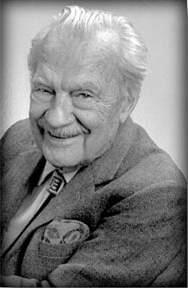
\includegraphics[scale=0.5]{metropolis}

\end{wrapfigure} Nicholas Constantine Metropolis (June 11, 1915 -- October 17, 1999)
was a Greek-American physicist.

Metropolis received his BSc (1937) and PhD (1941) degrees in physics
at the University of Chicago. Shortly afterwards, Robert Oppenheimer
recruited him from Chicago, where he was at the time collaborating
with Enrico Fermi and Edward Teller on the first nuclear reactors,
to the Los Alamos National Laboratory. He arrived in Los Alamos in
April 1943, as a member of the original staff of fifty scientists.

After World War II, he returned to the faculty of the University of
Chicago as an assistant professor. He came back to Los Alamos in 1948
to lead the group in the Theoretical Division that designed and built
the MANIAC I computer in 1952 that was modeled on the IAS machine,
and the MANIAC II in 1957. (He chose the name MANIAC in the hope of
stopping the rash of such acronyms for machine names, but may have,
instead, only further stimulated such use.) (John von Neumann thought
this acronym was too frivolous.) From 1957 to 1965 he was Professor
of Physics at the University of Chicago and was the founding Director
of its Institute for Computer Research. In 1965 he returned to Los
Alamos where he was made a Laboratory Senior Fellow in 1980.

In his memoirs, Stanislaw Ulam remembers that a small group, including
himself, Metropolis, Calkin, Konopinski, Kistiakowsky, Teller and
von Neumann, spent several evenings at Los Alamos playing poker. They
played for very small sums, but: \textquotedbl Metropolis once described
what a triumph it was to win ten dollars from John von Neumann, author
of a famous treatise on game theory. He then bought his book for five
dollars and pasted the other five inside the cover as a symbol of
his victory.\textquotedbl{} In another passage of his book, Ulam describes
Metropolis as \textquotedbl a Greek-American with a wonderful personality.\textquotedbl{}



\section{Wilfried Keith Hastings (source: Jeffrey Rosenthal's homepage).}

\begin{wrapfigure}{L}{0.25\textwidth} \centering

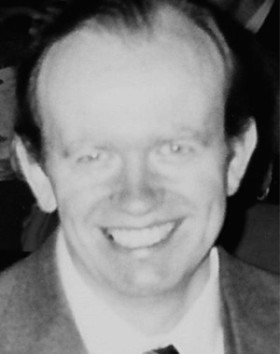
\includegraphics[scale=0.3]{hastings}

\end{wrapfigure} The Metropolis-Hastings algorithm (or, Hastings-Metropolis
algorithm) is the most common Markov chain Monte Carlo (MCMC) method.
It is extremely widely used in applied statistics and in statistical
physics and computer science and finance and more, to sample from
complicated, high-dimensional probability distributions. A primary
source for this algorithm is the paper:
\begin{itemize}
\item W.K. Hastings (1970), Monte Carlo sampling methods using Markov chains
and their applications. Biometrika 57, 97-109.
\end{itemize}
This paper has been cited well over two thousand times -{}- a huge
number. However, despite this paper's importance, very little information
about W.K. Hastings himself is publicly available. The following brief
biography is intended to (partially) answer that need.

W. Keith Hastings was born on July 21, 1930, in Toronto, Ontario,
Canada. He received his B.A. in Applied Mathematics from the University
of Toronto in 1953, and then worked from 1955-59 as a \textquotedbl Consultant
in Computer Applications\textquotedbl{} for the Toronto company H.S.
Gellman \& Co. Hastings recalls:

\emph{Harvey Gellman was a good mentor and encouraged me to pursue
my ideas. Some of the projects involved simulations and this was my
first contact with statistics and generation of samples from probability
distributions. }

Overlapping somewhat with this, Hastings received his M.A. in 1958,
and his Ph.D. in 1962, both from the University of Toronto's Department
of Mathematics (which included Statistics at that time). His Ph.D.
thesis title was \textquotedbl Invariant Fiducial Distributions\textquotedbl .
His Ph.D. supervisor was initially Don Fraser (who mentioned Hastings'
thesis results in a 1962 letter to R.A. Fisher), and later Geoffrey
Watson (while Fraser visited Stanford in 1961-62). After completing
his Ph.D., Hastings worked briefly at the University of Canterbury
in New Zealand (1962-64), and at Bell Labs in New Jersey (1964-66).
Hastings writes:

\emph{I was never comfortable working on statistical inference for
my thesis. My investigations led to too many dead ends and the work
seemed to involve more mathematical considerations than statistical
ones. When Geoff took over as my supervisor I briefly considered changing
topics, but ended up sticking with my original topic and completed
my thesis. In New Zealand, I continued this work for a while but eventually
gave it up, the final blow coming when I learned that Fiducial Probability
was declared 'dead' in a session during a statistics conference held
in Ottawa. Bell Labs provided a welcome and effective antidote to
all this as I gradually turned towards the computational aspects of
statistics. In effect, I was then returning to my professional roots. }

From 1966 to 1971, Hastings was an Associate Professor in the Department
of Mathematics at the University of Toronto. During this period, he
wrote the famous paper listed above (which generalised the work of
N. Metropolis, A. Rosenbluth, M. Rosenbluth, A. Teller, and E. Teller
(1953), \textquotedbl Equations of state calculations by fast computing
machines\textquotedbl , J. Chem. Phys. 21, 1087-1091). Hastings explains:

\emph{When I returned to the University of Toronto, after my time
at Bell Labs, I focused on Monte Carlo methods and at first on methods
of sampling from probability distributions with no particular area
of application in mind. {[}University of Toronto Chemistry professor{]}
John Valleau and his associates consulted me concerning their work.
They were using Metropolis's method to estimate the mean energy of
a system of particles in a defined potential field. With 6 coordinates
per particle, a system of just 100 particles involved a dimension
of 600. When I learned how easy it was to generate samples from high
dimensional distributions using Markov chains, I realised how important
this was for Statistics, and I devoted all my time to this method
and its variants which resulted in the 1970 paper.}

While at the University of Toronto, Hastings also supervised his one
Ph.D. student, Peter Peskun (now at York University), whose 1970 dissertation
\textquotedbl The Choice Of Transition Matrix In Monte Carlo Sampling
Methods Using Markov Chains\textquotedbl{} developed the Peskun ordering
on Markov chain kernels. Peskun recalls:

\emph{Dr. Hastings was down to earth and very good natured. I can
still picture him tugging at his waist band as he chuckled over some
comment he had just made. It was a pleasure having Dr. Hastings as
my Ph.D. supervisor. He never meddled in what I was trying to do but
was always happy to hear and listen to any new results that I came
up with. He did make one important suggestion to me which was to express
my initial heuristic results in matrix form. This was of tremendous
help in proving, in particular, Peskun orderings. }

In 1971, Hastings joined the Department of Mathematics at the University
of Victoria (in British Columbia, on the west coast of Canada) as
an Associate Professor, and was granted tenure there in 1974. He taught
at Victoria for 21 years, usually teaching six one-semester courses
per year. He did not supervise any more Ph.D. students, but he did
supervise two M.Sc. students, and serve on the committees of four
Ph.D. and two M.Sc. students. He held NSERC research grants from 1969
to 1980. Hastings' C.V. lists only two other refereed research papers
besides the famous (1970) one:
\begin{itemize}
\item W.K. Hastings (1972), Test Data for Statistical Algorithms: Least
Squares and ANOVA. J. Amer. Statist. Assoc. 67, 874-879.
\item W.K. Hastings (1974), Variance Reduction and Non-normality. Biometrika
61, 143-149.
\end{itemize}
It also lists one non-refereed publication (\textquotedbl Death and
Taxes\textquotedbl , American Studies in Papyrology 10, joint with
A.E. Samuel, A.K. Bowman, and R.S. Bagnall), and a couple of memoranda
for Bell Labs (including the suggestive-sounding \textquotedbl An
Overview of Statistical Computing Software\textquotedbl , 1966).
Hastings retired from the University of Victoria in 1992. He passed
away peacefully in Victoria on May 13, 2016, at the age of 85.

\end{subappendices}

\chapter{Geometric ergodicity and Central Limit theorems}

\minitoc
\begin{keywords}
Geometric Ergodicity, Coupling, Poisson equation, Martingales, Central Limit theorem.
\end{keywords}

\newcommand{\tvnorm}[1]{\left\|#1\right\|_{\mathrm{TV}}}
\newcommand{\coupling}{\mathcal{C}}

Let $(X_n)$ be a Markov chain with Markov kernel $P$ and assume that $P$ admits an invariant probability measure $\pi$. In this chapter, we are interested in finding conditions under which we can have bound of the error between the marginal distribution of $X_n$ and the distribution $\pi$. To do so, we first need to define some notion of "distance" between probability measures (we will define here the total variation distance). Then, we will compare $\pi$ and $P^n(x,\cdot)$, the distribution of the $n$-th iterate of the Markov kernel starting from an arbitrary point $x\in\Xset$, by bounding the total variation distance between them.


\section{Total variation norm and coupling}
\index{coupling}
We start with the notion of coupling between probability measures.
In words, if $\mu,\nu$ are two probability measures on $(\Xset,\Xsigma)$, then a coupling $\gamma$ of $(\mu,\nu)$ is a probability measure on the product space $(\Xset^2,\Xsigma^{\otimes 2})$ such that if $(X,Y) \sim \gamma$, then we have the marginal conditions: $X\sim\mu$ and $Y\sim \nu$.
\begin{shaded}
\begin{definition}
Let $(\Xset,\Xsigma)$ be a measurable space and let $\nu,\mu$ be two probability measures $\mu,\nu \in \meas 1(\Xset)$. We define $\coupling(\mu,\nu)$, the coupling set associated to $(\mu,\nu)$ as follows
$$
\coupling(\mu,\nu)=\set{\gamma\in\meas 1(\Xset^2)}{\forall A\in\Xsigma,\, \gamma(A\times\Xset)=\mu(A), \gamma(\Xset\times A)=\nu(A)}
$$
Any $\gamma\in\coupling(\mu,\nu)$ is called a coupling of $(\mu,\nu)$.
\end{definition}

\end{shaded}

Just to play with the definition of coupling, you can for example construct a coupling of $(\mu,\mu)$ by sampling $X\sim\mu$ and by setting $Y=X$. The distribution of $(X,Y)$ is then a coupling of $(\mu,\mu)$. This is a very "dependent" coupling (since we chose $X=Y$ by construction). We can also construct an "independent" coupling as follows: draw independently $X$ and $Y$ according to the same distribution $\mu$, then the distribution of $(X,Y)$ is a coupling of $(\mu,\mu)$ (since $X\sim \mu$ and $Y\sim \mu$).

But then, which coupling is interesting? As we shall see in what follows, there is a real degree of freedom for choosing an adequate coupling. We will present some useful couplings but there is no general rule.

Before going further into coupling techniques, let us define the total variation norm and let us link it with coupling.
\begin{shaded}
\begin{definition} \label{def:totvar}
\index{total variation distance}
Let $(\Xset,\Xsigma)$ be a measurable space and let $\nu,\mu$ be two probability measures $\mu,\nu \in \meas 1(\Xset)$. Then the total variation norm between $\mu$ and $\nu$ noted $\tvnorm{\mu-\nu}$, is defined by
\begin{align}
\tvnorm{\mu-\nu}&=2\sup\set{|\mu(f)-\nu(f)|}{f\in \funcset{}(\Xset), 0\leq f\leq 1} \label{eq:def:totvar:one}\\
&=\int |\varphi_0-\varphi_1|(x) \zeta(\rmd x) \label{eq:def:totvar:two}\\
&=2\inf\set{\PP(X\neq Y) }{ (X,Y) \sim \gamma \mbox{ where } \gamma \in \coupling(\mu,\nu)} \label{eq:def:totvar:three}
\end{align}
where $\mu(\rmd x)=\varphi_0(x) \zeta(\rmd x)$ and $\nu(\rmd x)=\varphi_1(x) \zeta(\rmd x)$.
\end{definition}

\end{shaded}

Before showing that these different expressions of the total variation are indeed equivalent, let us make a few comments.
\begin{leftbar}
\begin{enumerate}[(a)]
\item The reader might wonder why we can always write $\mu(\rmd x)=\varphi_0(x) \zeta(\rmd x)$ and $\nu(\rmd x)=\varphi_1(x) \zeta(\rmd x)$ for some well-chosen measure $\zeta$, and measurable functions $\varphi_0$ and $\varphi_1$. Actually, if we take $\mu,\nu \in \meas 1(\Xset)$, then setting $\zeta=\mu+\nu$ yields the two iimplications:
 $$
 \lr{\zeta(A)=0} \Longrightarrow \lr{\mu(A)=0} \quad \mbox{and} \quad   \lr{\zeta(A)=0} \Longrightarrow \lr{\nu(A)=0}
 $$
Therefore, the measure $\zeta$ dominates the measure $\mu$ and it also dominates the measure $\nu$. By the Radon Nikodym theorem, the measures $\mu$ and $\nu$ have densities wrt $\zeta$, densities that we call $\varphi_0$ and $\varphi_1$ in \Defref{totvar}.
\item The first definition, \eqref{eq:def:totvar:one}, is expressed as a supremum over functions, while the last one is an infimum over coupling measures... These two equalities can thus be considered as a {\em duality formula}.
\item The expression in the middle allows to write the total variation as a $L_1$-norm between the two densities of the distributions wrt to a common dominating measure.
\item An immediate consequence of the equivalent definitions of the total variation norm is that if $f$ is a measurable function taking values in $[0,1]$ and if $X,Y$ are random variables such that $(X,Y)\sim \gamma$ with $\gamma\in \coupling(\mu,\nu)$, then we have the coupling inequality \index{coupling!inequality}
$$
|\mu(f)-\nu(f)|\leq \PP(X\neq Y)
$$
This inequality will often be used in practice. It is due to such inequalities that coupling techniques are so successful.
\end{enumerate}
\end{leftbar}

\begin{svmultproof}[Proof of the equivalences in \Defref{totvar}] Call $A$, $B$ and $C$ the quantities that appear respectively in \eqref{eq:def:totvar:one}, \eqref{eq:def:totvar:two} and \eqref{eq:def:totvar:three}.
Any function $f$ satisfies $0\leq f\leq 1$ if and only if  the function $g=2f-1$ satisfies $|g| \leq 1$. This implies immediately
$$
A=2\sup\set{|\mu(f)-\nu(f)|}{f\in \funcset{}(\Xset), 0\leq f\leq 1}=\sup\set{|\mu(g)-\nu(g)|}{g\in \funcset{}(\Xset), |g|\leq 1}
$$
Moreover, for any $g\in \funcset{}(\Xset)$ such that $|g|\leq 1$,
$$
|\mu(g)-\nu(g)|=\left|\int (\varphi_1-\varphi_0)(x)g(x) \zeta(\rmd x) \right|\leq \int |\varphi_1-\varphi_0|(x)\underbrace{|g(x)|}_{\leq 1} \zeta(\rmd x)=B
$$
Therefore, $A\leq B$. Moreover, setting $g^*(x)=\mathrm{sign}(\varphi_0(x)-\varphi_1(x))$, we have $|g^*|=1$ and therefore,
\begin{align*}
B&=\int |\varphi_0-\varphi_1|(x) \zeta(\rmd x)=\int  \lr{\varphi_0(x)-\varphi_1(x)}{g^*(x)} \zeta(\rmd x)\\
 &= \mu(g^*) -\nu(g^*)\leq \sup\set{|\mu(g)-\nu(g)|}{g\in \funcset{}(\Xset), |g|\leq 1}=A
\end{align*}
Thus \fbox{$A=B$}. Now let $f\in \funcset{}(\Xset)$ be such that $0\leq f\leq 1$ and let $X,Y$ be random variables such that $(X,Y)\sim \gamma$ with $\gamma\in \coupling(\mu,\nu)$, then
$$
|\mu(f)-\nu(f)|=|\PE[f(X)-f(Y)]|=|\PE\lrb{\lrcb{f(X)-f(Y)}\indi{X\neq Y}}|\leq \PE[\underbrace{|f(X)-f(Y)|}_{\leq 1}\indi{X\neq Y}] \leq \PP(X\neq Y)
$$
This shows that \fbox{$A\leq C$}. To finish the proof, we will show that $C\leq B$ and to do so, we will exhibit an \textbf{optimal coupling} of $(\mu,\nu)$. \index{coupling!maximal}
\begin{leftbar}
Define
$$
\epsilon=\int_\Xset \varphi_0\wedge \varphi_1(x) \zeta(\rmd x) \quad \mbox{and} \quad  \zeta'(\rmd x)=\frac{\varphi_0\wedge \varphi_1(x) }{\epsilon}\zeta(\rmd x)
$$
Then, it can be readily checked that $\zeta'\in \meas{1}(\Xset)$, and $\mu(\rmd x)\geq \epsilon \zeta'(\rmd x)$ and $\nu(\rmd x)\geq \epsilon \zeta'(\rmd x)$. This implies that there exist $\mu_1,\nu_1\in\meas{1}(\Xset)$ such that
\begin{align*}
\mu(\rmd x)=\epsilon \zeta'(\rmd x) + (1-\epsilon) \mu_1(\rmd x)\\
\nu(\rmd x)=\epsilon \zeta'(\rmd x) + (1-\epsilon) \nu_1(\rmd x)
\end{align*}

\end{leftbar}

Define $\gamma(\rmd x\rmd y)=\epsilon \zeta'(\rmd x) \delta _x(\rmd y)+(1-\epsilon) \mu_1(\rmd x) \nu_1(\rmd y)$. Obviously, $\gamma \in \coupling(\mu,\nu)$. Let $X,Y$ be two random variables such that $(X,Y)\sim\gamma$. We can draw $(X,Y)$ in the following way: draw a Bernoulli variable $U\sim \mathrm{Ber}(\epsilon)$. If $U=1$, draw $X\sim\zeta'$ and set $Y=X$. If $U=0$, then draw independently $X\sim \mu_1$ and $Y\sim \nu_1$. Then, clearly
\begin{align*}
\PP(X\neq Y)&=1-\PP(X=Y) \leq 1-\epsilon=1-\int_\Xset \varphi_0\wedge \varphi_1(x) \zeta(\rmd x)\\
&=\frac{1}{2}\int_\Xset \underbrace{\varphi_0+ \varphi_1(x)-2 \varphi_0\wedge \varphi_1(x)}_{|\varphi_0- \varphi_1(x)|}\;\zeta(\rmd x)
\end{align*}
This shows that \fbox{$C\leq B$} and the proof is completed.
\end{svmultproof}

\begin{exercise}
Show that the supremum in \eqref{eq:def:totvar:one} is attained with a convenient choice of $f$.
\end{exercise}

Another equivalent expression of the total variation distance is
\begin{equation}\label{eq:coupling}
\tvnorm{\mu-\nu}= 2\inf\set{\gamma(\Delta) }{\gamma \in \coupling(\mu,\nu)}
\end{equation}
where we have used the notation $\Delta(x,y)=\indi{x\neq y}$ (we also say that $\Delta(x,y)$ is the Hamming distance between $x$ and $y$).

\begin{example}
See \autoref{eq:indice}.
  Let $\mu=\gauss(-1,1)$ and $\nu=\gauss(1,1)$. Let $X\sim \gauss(-1,1)$ and set $Y=X+2$. Then,
  $(X,Y)$ is a coupling of $(\mu,\nu)$ but it is not the optimal coupling for the Hamming distance
  since $\PP(X\neq Y) = 1$, whereas using \Defref{totvar},
  \begin{align*}
    \tvnorm{\mu-\nu} = 2\lr{1 - \int_{-\infty}^\infty \phi(x+1)\wedge\phi(x-1) \rmd x} =2\lr{
1 -     2 \int_1^\infty \frac{\rme^{-u^2/2}}{\sqrt{2\pi}} \rmd u }\eqsp ,
  \end{align*}
  where $\phi$ the density of the standard Gaussian distribution.

\begin{figure}[!h]
\begin{center}
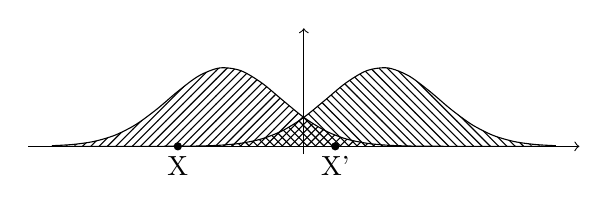
\begin{tikzpicture}[domain=-3.2:3.2]
\draw[very  thin,color=gray]  (-3,-0.1)   (3,1.1);
\draw[smooth, pattern= north west lines] plot(\x,{exp(-((\x-1)^2))});
\draw[smooth, pattern= north east lines]     plot (\x,{exp(-((\x+1)^2))});
\draw[->]  (-3.5,0)  --  (3.5,0);
\draw[->]  (0,-0.1)  --  (0,1.5);
\fill(-1.6,0)circle(1.5pt) node[below]{X};
\fill(0.4,0)circle(1.5pt) node[below]{X'};


\end{tikzpicture}
\end{center}

\caption{An example of coupling of two probability measures.}
\label{eq:indice}
\end{figure}

\end{example}
\section{Geometric ergodicity}
In what follows, we assume that for {\bf some measurable function $V:\Xset \to [1,\infty)$}, we have

\begin{shaded}
\begin{hyp}{A}
\item\label{assum:Aone} [{\bf Minorizing condition}] for all $d>0$, there exists $\epsilon_d>0$ and a probability measure $\nu_d$ such that \index{minorizing condition}
\begin{equation}
\label{eq:minor}
\forall x\in C_d\eqdef\{V\leq d\}, \quad
P(x,\cdot) \geq \epsilon_d \nu_d(\cdot)
\end{equation}
\end{hyp}

\end{shaded}

\begin{shaded}
\begin{hyp}{A}
\item\label{assum:Atwo} [{\bf Drift condition}] \index{drift condition}there exists a constants $(\lambda,b)\in (0,1) \times \rset^+$ such that for all $x\in\Xset$,
$$
PV(x) \leq \lambda V(x)+b
$$
\end{hyp}

\end{shaded}

Typically, the function $V$ is unbounded (but in particular situations, it can also be bounded) and the level set $\{V\leq d\}$ is typically compact (when the chain takes value a topological space)... Roughly speaking, \ref{assum:Aone} tells you that wherever $x$ moves in a set $C_d$, the measure $P(x,\cdot)$ is lower bounded by the non-trivial measure $\epsilon_d \nu_d(\cdot)$. In many cases, $\Xset=\rset^n$, and $P$ is dominated by the Lebesgue measure: $P(x,\rmd y)=p(x,y)\rmd y$. In that case, we usually take $P(x,A)\geq \epsilon_d  \nu_d(A)$ where
$$
 \epsilon_d=\int_\Xset \lrb{\inf_{x\in C_d}p(x,y)}\rmd y, \quad \nu_d(A)=\frac{\int_A \inf_{x\in C_d}p(x,y)\rmd y}{\epsilon_d}
$$
i.e. we only need to bound from below the kernel density $p(x,y)$ when $x\in C_d$. If $C_d$ is compact, then it is quite easy to check such lower-bound. In the Markov chain terminology, if   \eqref{eq:minor} holds, we say that $C_d$ is a small set. \index{small set}

The drift condition \ref{assum:Atwo} tells you that in the mean sense, the drift function $V$ is shrinked by a factor $\lambda$ up to the additive constant $b$... Intuitively speaking, the Markov kernel $P$ does not bring to regions where $V$ is too large so that the chain does not go to infinity too quickly (since limited values of $V$ corresponds typically to bounded sets). And we can easily  imagine that such chains will have nice ergodic properties.

Before stating the result, we must say that, in practise, for a given Markov kernel $P$, there is no general rule for guessing the expression of a drift function $V$ that satisfies \ref{assum:Atwo}, and we have to try different functions $V$ for checking the assumptions... For example, if $X_{k+1}=\alpha X_k+\epsilon_k$ where $(\epsilon_k)$ are iid and $\alpha\in (0,1)$. If we know that $\PE[|\epsilon_1|^r]<\infty$, then we can try a drift function $V(x)=|x|^r$ and if $\PE[\rme^{\beta \epsilon_1}]<\infty$, then we can  try $V(x)=\rme^{\beta x}$. For MH algorithms, we also sometimes use a negative power of the target density. But once again, the choice of $V$ is very model specific (and in some sense, this is a good opportunity to be imaginative!!!).
We now show that assumptions \ref{assum:Aone} and \ref{assum:Atwo} imply that the Markov kernel $P$ is "geometrically ergodic" in the following sense.
\begin{shaded}
\begin{theorem}\label{thm:ergo:geom} [{\bf Geometric ergodicity}] \index{geometric ergodicity}
Assume \ref{assum:Aone} and \ref{assum:Atwo}\ for some measurable function $V\geq1$.
Then, there exists a constant $\varrho \in (0,1)$ such that for all $x,x'\in\Xset$ and all $n\in\nset$,
$$
\tvnorm{P^n(x,\cdot)-P^n(x',\cdot)} \leq \varrho^n \lrb{V(x)+V(x')}  .
$$
\end{theorem}
\end{shaded}
\begin{remark}
Assume that there exist a constant $\epsilon>0$ and a probability measure $\nu$ such that for all $x\in\Xset$, $P(x,\cdot)\geq \epsilon \nu(\cdot)$. In that case, \ref{assum:Aone} and \ref{assum:Atwo} are satisfied with the constant function $V(x)=1$ and \autoref{thm:ergo:geom} then shows that
$$
\tvnorm{P^n(x,\cdot)-P^n(x',\cdot)} \leq 2 \varrho^n  .
$$
for some constant $\varrho\in(0,1)$. Such a Markov chain is usually said to be uniformly ergodic.
\end{remark}
The proof needs several steps. To bound $\tvnorm{P^n(x,\cdot)-P^n(x',\cdot)}$, we will construct a bivariate Markov chain $(X_k,X'_k)$ such that first component process $(X_k)$ behaves marginally as a Markov chain starting from $x$ with Markov kernel $P$, while the second component process $(X_k)$ behaves marginally as a Markov chain starting from $x'$ with Markov kernel $P$. Let us be more specific...
 In what follows, we choose $d$ sufficiently large so that
 \begin{equation}\label{eq:def:barlambda}
 \bar \lambda \eqdef \lambda +\frac{2b}{1+d}<1
 \end{equation}
\subsubsection*{Definition of the joint kernel $\bar P$}
Define $Q(x_k,\rmd x_{k+1})=\frac{P(x_k,\rmd x_{k+1})-\epsilon_d \nu_d(\rmd x_{k+1})}{1-\epsilon_d}$ and set
\begin{align*}
&\bar P( (x_k,x_k'),\rmd x_{k+1} \rmd x'_{k+1})=\indi{x_k=x'_k}P(x_k,\rmd x_{k+1})  \delta_{x_{k+1}} (x'_{k+1}) \\
&\quad + \indi{x_k\neq x'_k } \indi{(x_k,x'_k)\notin C_d^2 }\lrb{P(x_k,\rmd x_{k+1})P(x'_k,\rmd x'_{k+1})}\\
&\quad + \indi{x_k\neq x'_k } \indi{(x_k,x'_k)\in C_d^2 }\lrb{\epsilon_d \nu_d(\rmd x_{k+1})\delta_{x_{k+1}} (x'_{k+1})+(1-\epsilon_d)Q(x_k,\rmd x_{k+1})Q(x'_k,\rmd x'_{k+1})}\
\end{align*}
Actually, $\bar P$ is a Markov kernel on $\Xset^2 \times \Xsigma^{\otimes 2}$ and it can be easily checked that
\begin{equation}
\bar P((x,x'),\cdot) \in \coupling (P(x,\cdot),P(x',\cdot))
\end{equation}
This will indeed imply by induction that for any $n\in\nset$,
\begin{equation} \label{eq:coupling:n}
\bar P^n((x,x'),\cdot) \in \coupling (P^n(x,\cdot),P^n(x',\cdot))
\end{equation}


%Denote by $\bar \PP_{x,x'}$ the probability measure induced on $( (\Xset^2)^\nset,(\Xsigma^{\otimes 2})^{\otimes \nset})$ by the Markov kernel $\bar P$ starting from $(x,x')$.

\subsubsection*{Interpretation of the joint kernel $\bar P$}
Set $\bar X_k=(X_k,X'_k)$ and $\bar C_d=C_c\times C_d$. If $(\bar X_k)_{k\in\nset}$ is a Markov chain with the Markov kernel $\bar P$, the transition from $\bar X_k=(x_k,x'_k)$ to $\bar X_{k+1}=(X_{k+1},X'_{k+1})$ can be seen as follows
\begin{itemize}
\item If $x_k=x'_k$, draw $X_{k+1}\sim P(x_k,\cdot)$ and set $X'_{k+1}=X_{k+1}$.
\item Otherwise,
\begin{itemize}
\item If $(x_k,x'_k) \notin \bar C_d$, then
\begin{itemize}
\item Draw independently $X_{k+1}\sim P(x_k,\cdot)$ and $X'_{k+1}\sim P(x'_k,\cdot)$
\end{itemize}
\item If $(x_k,x'_k) \in \bar C_d$, then
\begin{itemize}
\item Draw $U\sim \mathrm{Ber}(\epsilon_d)$.
\item If $U=1$, draw $X_{k+1}\sim \nu_d$ and set $X'_{k+1}=X_{k+1}$.
\item If $U=0$, draw independently $X_{k+1}\sim Q(x_k,\cdot)$ and $X'_{k+1}\sim Q(x'_k,\cdot)$.
\end{itemize}
\end{itemize}
\item Set $\bar X_{k+1}=(X_{k+1},X'_{k+1})$.
\end{itemize}
Therefore, the bivariate Markov chain $(\bar X_k)_{k\in\nset}=(X_k,X'_k)_{k\in\nset}$  is such that it tries to couple its two components with probability $\epsilon_d$ each time it falls into $\bar C_d$ and once it couples (ie $X_k=X'_k$) then, it stays together for ever (ie for all $n\geq k$, $X_n=X'_n$).
\subsubsection*{Some nice properties of $\bar P$}
The following inequalities are immediate:
\begin{enumerate}
\item Set $\Delta(x,x')=\indi{x\neq x'}$, then
\begin{enumerate}[(a)]
\item if $(x,x') \in \bar C_d$, $\bar P \Delta(x,x') \leq (1-\epsilon_d) \Delta(x,x')$
\item if $(x,x') \notin \bar C_d$, $\bar P \Delta(x,x') \leq \Delta(x,x')$
\end{enumerate}
\item Setting $\bar V(x,x')=(V(x)+V(x'))/2$, we have $\bar P \bar V(x,x')=2^{-1}(PV(x)+PV(x'))\leq \lambda \bar V(x,x')+b$. This implies
\begin{enumerate}[(a)]
\item if $(x,x') \in \bar C_d$, $\bar P \bar V(x,x') \leq (\lambda+b) \bar V(x,x')$
\item if $(x,x') \notin \bar C_d$, $\bar P \bar V(x,x') \leq \big(\underbrace{\lambda+\frac{2b}{1+d}}_{\bar \lambda}\big)\bar V(x,x')$
\end{enumerate}
\end{enumerate}
%We can sum up the first item by:
%\begin{equation} \label{eq:erg:first}
%\bar P \Delta(x,x') \leq (1-\epsilon_d)^{\indi{\bar C_d}(x,x')} \Delta(x,x')
%\end{equation}
%Similarly the second item can be sum up by:
%\begin{equation}\label{eq:erg:second}
%\bar P \bar V(x,x') \leq (\lambda +b)^{\indi{\bar C_d}(x,x')} \bar \lambda^{1-\indi{\bar C_d}(x,x')}\bar V(x,x')
%\end{equation}
%Actually instead of considering $\bar V(x,x')$ we will consider the function  $\Delta V: (x,x')\mapsto \indi{x\neq x'} V(x,x')$. Then, we have:
%\begin{equation} \label{eq:erg:third}
%\bar P (\Delta\bar V)(x,x') \leq (\lambda +b)^{\indi{\bar C_d}(x,x')} \bar \lambda^{1-\indi{\bar C_d}(x,x')}(\Delta\bar V)(x,x')
%\end{equation}
%To see this, we distinguish the two cases:
%\begin{itemize}
%\item either $x=x'$, then $\bar P (\Delta\bar V)(x,x')=0$ and  \eqref{eq:erg:third} holds true since the lhs and rhs are null.
%\item or $x\neq x'$, then, using $\Delta\leq 1$,  and $\Delta(x,x')=1$
%$$
%\bar P (\Delta\bar V)(x,x')\leq \bar P \bar V(x,x')\leq  (\lambda +b)^{\indi{\bar C_d}(x,x')} \bar \lambda^{1-\indi{\bar C_d}(x,x')}\underbrace{\bar V(x,x')}_{\Delta \bar V(x,x')}
%$$
%\end{itemize}

We now have all the tools for proving \autoref{thm:ergo:geom}.
\begin{svmultproof}[of  \autoref{thm:ergo:geom}]

For any $\beta\in (0,1)$, define
\begin{equation}
\varrho_\beta=\max((1-\epsilon_d)^{1-\beta} (\lambda +b)^\beta, \bar \lambda^{\beta})
\end{equation}
The expression of $\varrho_\beta$ may seem a bit complicated (we will understand why we choose $\varrho_\beta$ like this in \eqref{eq:W} below) but, since $\bar \lambda$ and $1-\epsilon_d$ are both in $(0,1)$, we can always pick $\beta$ sufficiently small (but positive) so that \fbox{$\varrho_\beta \in (0,1)$}. This $\varrho_\beta$ being chosen, set $W=\Delta^{1-\beta} \bar V^\beta$.
Then, using Holder's inequality and the inequalities in the section \textbf{Some nice properties of} $\bar P$, we have for all $(x,x')\in\Xset^2$,
\begin{align*}
\bar PW(x,x')=\bar P(\Delta^{1-\beta} \bar V^\beta )(x,x') &\leq (\bar P \Delta (x,x'))^{1-\beta} (\bar P \bar V (x,x'))^\beta \\
& \leq (\Delta^{1-\beta} \bar V^\beta) (x,x') \times \begin{cases}
(1-\epsilon_d)^{1-\beta} (\lambda +b)^\beta &\mbox{if $(x,x')\in C_d^2$} \\
\bar \lambda^{\beta}  &\mbox{if $(x,x')\notin C_d^2$}
\end{cases}\\
&\leq \varrho_\beta  W (x,x')
\end{align*}
This implies by induction that for all $n\in\nset$ and all $(x,x')\in\Xset^2$,
\begin{equation}\label{eq:W}
\bar P^nW(x,x') \leq \varrho^n_\beta  W (x,x')
\end{equation}
Then
\begin{align*}
& \tvnorm{P^n(x,\cdot)-P^n(x',\cdot)}  \stackrel{(1)}{\leq} 2 \bar P^n \Delta(x,x') \stackrel{(2)}{\leq} 2 \bar P^n W(x,x') \stackrel{(3)}{\leq} 2\varrho_\beta^n W(x,x') \stackrel{(4)}{\leq} \varrho_\beta^n (V(x)+V(x'))
\end{align*}
where $(1)$ comes from \eqref{eq:coupling:n} and \eqref{eq:coupling}, $(2)$ from  $\Delta(x,x')=\Delta^{1-\beta}(x,x')\leq W(x,x')$ because $V\geq 1$, $(3)$ from \eqref{eq:W}
and $(4)$ from
$$
W(x,x')\leq \lr{\frac{V(x)+V(x')}{2}}^{\beta} \leq \frac{V(x)+V(x')}{2}
$$
since $V\geq 1$ and $\beta\in(0,1)$.
\end{svmultproof}


\begin{corollary} \label{cor:ergod}
Assume that \ref{assum:Aone} and \ref{assum:Atwo}\ hold for some measurable function $V\geq 1$. Then, the Markov kernel $P$ admits a unique invariant probability measure $\pi$. Moreover, $\pi(V)<\infty$ and there exists constants $(\varrho,\alpha) \in (0,1) \times \rset^+$ such that for all $\mu\in\meas 1(\Xset)$ and all $n\in\nset$,
$$
\tvnorm{\mu P^n-\pi} \leq \alpha \varrho^n \mu(V)  .
$$
\end{corollary}
\begin{svmultproof}
For any $\mu,\nu \in\meas 1(\Xset)$ and any $h\in\funcset(\Xset)$ such that $|h|\leq 1$,  we have, using \autoref{thm:ergo:geom},
$$
|\mu P^n h-\nu P^n h|=|\int_{\Xset^2}\mu(\rmd x)\nu(\rmd y) [P^nh(x)-P^nh(y)]| \leq \int_{\Xset^2}\mu(\rmd x)\nu(\rmd y)| [P^nh(x)-P^nh(y)]| \leq \varrho^n [\mu(V) +\nu(V)]
$$
Thus,
\begin{equation}\label{eq:totVar:fond}
\tvnorm{\mu P^n -\nu P^n}\leq \varrho^n [\mu(V) +\nu(V)]
\end{equation}
Replacing $\mu$ by $\delta_x$ and $\nu$ by $P(x,\cdot)$, we get for all $x\in\Xset$,
$$
\tvnorm{P^n(x,\cdot) -P^{n+1}(x,\cdot)}\leq \varrho^n [V(x) +PV(x)] \leq \varrho^n [(1+\lambda) V(x)+b]
$$
This implies that $\{P^n(x,\cdot)\}$ is a Cauchy sequence and since $(\meas 1(\Xset),\tvnorm \cdot)$ is complete, it converges to a limit $\pi \in\meas 1(\Xset)$. Then, for all $x\in\Xset$ and all  $h\in\funcset{}(\Xset)$ such that $|h|\leq 1$, we also have $|Ph|\leq 1$ and therefore
$$
\pi(Ph)=\lim_{n\to\infty} P^n (Ph)(x)=\lim_{n\to\infty} P^{n+1}h(x)=\pi(h)
$$
showing that $\pi$ is $P$-{\bf invariant}. We now show {\bf uniqueness} of an invariant probability measure. To see this, note that $\pi$ actually does not depend on the choice of $x$. Indeed, replacing $\mu$ by $\delta_x$ and $\nu$ by $\delta_{x'}$ in \eqref{eq:totVar:fond}, we get that $\lim_{n\to\infty}\tvnorm{P^n(x,\cdot) -P^{n}(x',\cdot)}=0$. Therefore, for all $x\in\Xset$, $\lim_{n\to\infty} P^{n}h(x)=\pi(h)$. Let $\pi'$ be an invariant probability measure for $P$, then
$$
\pi'(h)=\pi' P^n(h)=\int \pi'(\rmd x) \underbrace{P^n h(x)}_{\to \pi(h)} \rightarrow_{n\to\infty} \pi(h)
$$
where the last equality comes from Lebesgue's dominated convergence theorem. Since $PV\leq \lambda V+b$, we have by induction for all $n\in\nset$,
$$
P^n V(x)\leq \lambda^n V(x)+b \lr{\sum_{k=0}^{n-1}\lambda^k} \leq \lambda^n V(x)+\frac{b}{1-\lambda}
$$
Therefore, for any $M>0$, by Jensen's inequality applied to the convex function $u\mapsto u\wedge M$, we have $P^n (V\wedge M)(x) \leq ( P^n V(x))\wedge M \leq \lr{\lambda^n V(x)+\frac{b}{1-\lambda}} \wedge M$. We then integrate wrt $\pi$ and use $\pi=\pi P^n$:
$$
\pi(V\wedge M)=\pi P^n(V\wedge M) \leq \int \pi(\rmd x) \lr{\lambda^n V(x)+\frac{b}{1-\lambda}} \wedge M
$$
The Lebesgue dominated convergence theorem then shows by letting $n$ to infinity, $\pi(V\wedge M)\leq \frac{b}{1-\lambda} \wedge M$. Then, letting $M$ to infinity, we get $\pi(V)\leq b/(1-\lambda)<\infty$. To complete the proof, apply \eqref{eq:totVar:fond} with $\nu=\pi$, we get
$$
\|\mu P^n -\underbrace{\pi P^n}_{\pi}\|_{\mathrm{TV}}\leq \varrho^n [\mu(V) +\pi(V)]\leq \alpha \varrho^n [\mu(V)
$$
with $\alpha=1+\pi(V)<\infty$.
\end{svmultproof}


Exercise~\ref{exo:LLN:Aone:Atwo} shows that under \ref{assum:Aone} and \ref{assum:Atwo} a Law of Large number is valid, starting from any initial distribution.

\autoref{cor:ergod} is nice but it is expressed only as a bound on the total variation norm, this implies that we can bound $|\mu P^n h -\pi(h)|$ where $|h|\leq 1$. Under the same assumptions, we can actually obtain more general bounds for possibly unbounded functions $h$. The proof is slightly more complicated so we decide to just state the result.

\begin{shaded}
\begin{theorem} \label{thm:ergo:gener}
 Assume that \ref{assum:Aone} and \ref{assum:Atwo}\ hold for some function $V\geq 1$. Then, there exist constants $(\varrho,\alpha) \in (0,1) \times \rset^+$ such that for all $\mu\in\meas 1(\Xset)$ satisfying $\mu(V)<\infty$, all $n\in\nset$ and all measurable functions $|h|\leq V$,
$$
|\mu P^n h -\pi(h)| \leq \alpha \varrho^n \mu(V)\eqsp.
$$
\end{theorem}

\end{shaded}

\section{The Poisson Equation}
\subsection{Definition}
We start with a general definition of a Poisson equation.
\begin{framed}
\begin{definition} \index{Poisson equation}
For a given measurable function $h$ such that $\pi|h|<\infty$, the Poisson equation is defined by
\begin{equation} \label{eq:Poisson}
\hat h - P \hat h=h-\pi(h)
\end{equation}
A solution to Poisson equation \eqref{eq:Poisson} is a function $\hat h$ such that $P|\hat h|(x)<\infty$ for all $x\in\Xset$ and for all $x\in\Xset$, $\hat h(x) - P \hat h(x)=h(x)-\pi(h)$.

\end{definition}
\end{framed}
The following result holds under the set of assumptions \ref{assum:Aone} and \ref{assum:Atwo}.
\begin{shaded}
 \begin{theorem} \label{thm:solPoiss}
 Assume \ref{assum:Aone} and \ref{assum:Atwo} hold for some measurable function $V\geq 1$. Then, for any function $h$ such that $|h|\leq V$, the function
\begin{equation}\label{eq:solPoisson}
\hat h=\sum_{n=0}^\infty \lrcb{P^n h-\pi(h)}
\end{equation}
is well-defined. Moreover, $\hat h$ is a solution of the Poisson equation associated to $h$ and there exists a constant $\gamma$ such that  for all $x\in\Xset$,
$$
|\hat h(x)|\leq \gamma V(x)
$$
 \end{theorem}

\end{shaded}

 \begin{svmultproof}
To see the existence of a solution to the Poisson equation under \ref{assum:Aone} and \ref{assum:Atwo}, note that by \autoref{thm:ergo:gener}, $\sum_{n=0}^\infty \lrcb{P^n h(x)-\pi(h)}$ converges for any $|h|\leq V$ and we can thus define
\begin{equation*}
\hat h(x)=\sum_{n=0}^\infty \lrcb{P^n h(x)-\pi(h)}
\end{equation*}
Then,
$$
P \hat h(x)=\sum_{n=1}^\infty \lrcb{P^n h(x)-\pi(h)}
$$
which immediately shows \eqref{eq:Poisson}. Moreover, setting $\hat h$ as in \eqref{eq:solPoisson}, \autoref{thm:ergo:gener} shows that for all $x\in\Xset$,
$$
|\hat h(x)|\leq \frac{\alpha}{1-\varrho} V(x)
$$
 \end{svmultproof}




\subsection{Poisson equation and martingales}

The interest of Poisson equation is that it allows to link quantities of interest of our Markov chain with a well-chosen martingale. Then, we apply limiting results on martingales and the impact of those results to our Markov chain.

We start with a refresher on martingales.

\subsubsection{A refresh on martingales}
\index{martingales}
Let $(M_n)_{n \in \nset}$ be a sequence of random variables on the same probability space $(\Omega,\mcf,\PP)$ and let $(\mcf_n)_{n\in\nset}$ be a filtration (ie for all $n\in\nset$, $\mcf_n\subset \mcf_{n+1}\subset \mcf$). We say that $(M_n)_{n \in \nset}$ is a {\rm $(\mcf_n)$-martingale} if for all $n\in\nset$, $M_n$ is integrable and for all $n\geq 1$,
$$
\PE[M_n|\mcf_{n-1}]=M_{n-1}
$$
The {\em increment process} of the martingale is by definition $(M_{n+1}-M_n)_{n\in\nset}$.

The following CLT result holds for martingales with stationary increments. It is stated without proof.
\begin{framed}
\begin{theorem} \label{thm:clt:marting} \index{martingales!central limit theorem}
If a sequence $(M_n)_{n \in \nset}$ is a $(\mcf_n)$-martingale with stationary and square integrable increments, then
$$
  n^{-1/2} M_n \dlim{\PP} \gauss\lr{0,\PE[(M_1-M_0)^2]}
$$
\end{theorem}

\end{framed}

\subsubsection{Link with martingales}

Define
$$
S_n(h)=\sum_{k=0}^{n-1} \lrcb{h(X_k)-\pi(h)}
$$
The solution of the Poisson equation allows us to relate $S_n(h)$ to a martingale by writing:
\begin{equation}\label{eq:decomp:marting}
S_n(h)=M_n(\hat h)+\hat h(X_0)-\hat h(X_n)
\end{equation}
where
\begin{equation}\label{eq:def:marting}
M_n(\hat h)=\sum_{k=1}^n \lrcb{\hat h(X_k)-P\hat h(X_{k-1})}
\end{equation}
Note that $\lrcb{M_n(\hat h)}_{n\in\nset}$ is indeed a $(\mcf_k)$-martingale where $\mcf_k=\sigma(X_0,\ldots,X_k)$ since:
$$
\PE[M_n(\hat h)|\mcf_{n-1}]-M_{n-1}(h)=\PE[\hat h(X_n)-P\hat h(X_{n-1})|\mcf_{n-1}]=P\hat h(X_{n-1})-P\hat h(X_{n-1})=0
$$
This link with martingales allows to obtain LLN and Central Limit theorems for our Markov chain from limiting results on martingales. Since LLN has been already studied in a different approach in the previous chapter, we only focus here on CLT.


\subsection{Central Limit theorems}

\begin{shaded}
 \begin{theorem}
  \label{thm:clt-poisson} \index{central limit theorem}
  Let $P$ be a  Markov kernel with a unique invariant probability measure $\pi$. Let
  $h \in \ltwo(\pi)$. Assume that there exists a solution
  \fbox{$\hat{h} \in \ltwo(\pi)$} to the Poisson equation $\hat{h} - P \hat{h} = h$. Then
  \begin{align*}
    n^{-1/2} \sum_{k=0}^{n-1} \{h(X_k)-\pi(h)\} \dlim{\PP_\pi} \gauss(0,\sigma_\pi^2(h)) \eqsp ,
  \end{align*}
  where
  \begin{equation}
  \label{eq:equality-variance}
  \sigma_\pi^2(h) = \PE_\pi[ \{\hat{h}(X_1)-P\hat{h}(X_0)\}^2] %= \pi(\hat{h}^2 - (P\hat{h})^2)
%  = 2 \pi(h\hat{h})-\pi(h^2) \eqsp.
  \end{equation}
\end{theorem}

\end{shaded}

\begin{svmultproof}
Without loss of generality, we assume $\pi(h)=0$.
  The sequence $(M_n(\hat h))_{n \in \nset}$ defined in
  \eqref{eq:def:marting} is such that
  \begin{multline*}
\PE_\pi[(M_n(\hat h)-M_{n-1}(\hat h))^2]=\PE_\pi[ \{\hat{h}(X_1)-P\hat{h}(X_0)\}^2] \leq 2 \PE_\pi[ \hat{h}^2(X_1)+(P\hat{h}(X_0))^2]  \\
= 2 \lrb{\pi(\hat h^2) +\pi( (P\hat h)^2)}  \stackrel{(1)}{\leq} 2 \lrb{\pi(\hat h^2) +\underbrace{\pi P}_{\pi}(\hat h)^2}=2\pi(\hat h^2)<\infty
  \end{multline*}
  where $\stackrel{(1)}{\leq}$ follows from Cauchy-Schwarz inequality.
 Therefore,  the sequence $(M_n(\hat h))_{n \in \nset}$ is a martingale with stationary and square integrable increments under $\PP_\pi$. By \autoref{thm:clt:marting}, we have
  \begin{equation} \label{eq:convMarting}
  n^{-1/2} M_n(\hat h) \dlim{\PP_\pi} \gauss\left(0, \PE_\pi[ \{\hat{h}(X_1)-P\hat{h}(X_0)\}^2] \right) \eqsp.
  \end{equation}
 Since the Markov chain $(X_k)_{k\in\nset}$ is stationary under $\PP_\pi$, we get
  $\PE_\pi[|\hat{h}(X_0)+\hat{h}(X_n)|] \leq 2 \pi(|\hat{h}|)$ which implies that
  \[
  n^{-1/2} \{\hat{h}(X_0)+\hat{h}(X_n)\}\plim{\PP_\pi}0 \eqsp.
  \]
Combining it with \eqref{eq:convMarting} and \eqref{eq:decomp:marting} and using Slutsky's lemma gives:
$$
    n^{-1/2} \sum_{k=0}^{n-1} h(X_k) \dlim{\PP_\pi} \gauss(0,\sigma_\pi^2(h))
$$
\end{svmultproof}

\begin{shaded}
\begin{theorem} \label{thm:clrHairer}
Assume that \ref{assum:Aone} and \ref{assum:Atwo}\ hold for some function $V$. Then, for all measurable functions $h$ such that $|h|^2\leq V$,
  \begin{align*}
    n^{-1/2} \sum_{k=0}^{n-1} \{h(X_k)-\pi(h)\}  \dlim{\PP_\pi} \gauss(0,\sigma_\pi^2(h)) \eqsp ,
  \end{align*}
  where
  \begin{equation}
  \label{eq:equality-variance}
  \sigma_\pi^2(h) = \PE_\pi[ \{\hat{h}(X_1)-P\hat{h}(X_0)\}^2] %= \pi(\hat{h}^2 - (P\hat{h})^2)
%  = 2 \pi(h\hat{h})-\pi(h^2) \eqsp.
  \end{equation}
and $\hat h$ is defined as in \eqref{eq:solPoisson}.
\end{theorem}

\end{shaded}

\begin{svmultproof}
Assume that \ref{assum:Aone} and \ref{assum:Atwo}\ hold for some function $V$. Then, \ref{assum:Aone} also holds with $V$ replaced by $V^{1/2}$. Moreover, since $PV\leq \lambda V +b$, we have by Cauchy-Schwarz,
$$
P(V^{1/2}) \leq (PV)^{1/2}\leq (\lambda V +b)^{1/2}\leq  \lambda^{1/2} V^{1/2}+b^{1/2}
$$
Finally, \ref{assum:Aone} and \ref{assum:Atwo}\ hold for the function $V^{1/2}$. We can therefore apply \autoref{thm:solPoiss} with $V$ replaced by $V^{1/2}$. Then, for all $h\leq V^{1/2}$, the function $\hat h$ defined by \eqref{eq:solPoisson} is solution to the Poisson equation and there exists a constant $\gamma>0$ such that
$\hat h\leq \gamma V^{1/2}$. This implies that $\pi(\hat h^2) \leq \gamma \pi(V)<\infty$ by \autoref{cor:ergod}. Therefore $\hat{h} \in \ltwo(\pi)$ and  \autoref{thm:clt-poisson} applies. The proof is completed.
\end{svmultproof}

Under the assumptions of \autoref{thm:clrHairer}, the CLT holds under $\PP_\pi$. We can actually extend this result to all $\PP_\nu$ where $\nu$ is any probability measure in $\meas 1(\Xset)$.
\section{After studying this chapter...}
\begin{center}
\shadowbox{\begin{minipage}{0.9\textwidth}
\begin{enumerate}[a)]
\item I understand the three expressions of the total variation norm.
\item If asked, I can try to prove that a Markov kernel is geometrically ergodic by checking the minorizing condition and the drift condition.
\item I understand the coupling inequality.
\item I understand the proof of \autoref{thm:ergo:geom}, which is hard but also beautiful...
\item I know what is a Poisson equation and I can write a solution of the Poisson equation as a series.
\item I understand in what sense Poisson equation allows to establish links between Markov Chains and martingales.
\end{enumerate}
\end{minipage}
}
\end{center}



\section*{Highlights}

\begin{subappendices}

\section{Stanislaw Ulam (source: wikipedia).}

\begin{wrapfigure}{L}{0.25\textwidth} \centering

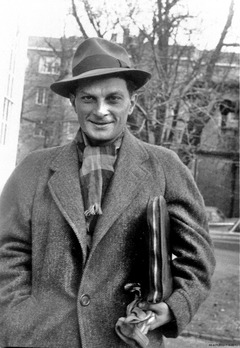
\includegraphics[scale=1.5]{ulam}

\end{wrapfigure}
Stanislaw Marcin Ulam (3 april 1909-13 may 1984) was a Polish-American scientist in the fields of mathematics and nuclear physics. He participated in the Manhattan Project, originated the Teller-Ulam design of thermonuclear weapons, discovered the concept of the cellular automaton, invented the Monte Carlo method of computation, and suggested nuclear pulse propulsion. In pure and applied mathematics, he proved some theorems and proposed several conjectures.

Born into a wealthy Polish Jewish family, Ulam studied mathematics at the Lwow Polytechnic Institute, where he earned his PhD in 1933 under the supervision of Kazimierz Kuratowski. In 1935, John von Neumann, whom Ulam had met in Warsaw, invited him to come to the Institute for Advanced Study in Princeton, New Jersey, for a few months. From 1936 to 1939, he spent summers in Poland and academic years at Harvard University in Cambridge, Massachusetts, where he worked to establish important results regarding ergodic theory. On 20 August 1939, he sailed for the United States for the last time with his 17-year-old brother Adam Ulam. He became an assistant professor at the University of Wisconsin-Madison in 1940, and a United States citizen in 1941.

In October 1943, he received an invitation from Hans Bethe to join the Manhattan Project at the secret Los Alamos Laboratory in New Mexico. There, he worked on the hydrodynamic calculations to predict the behavior of the explosive lenses that were needed by an implosion-type weapon. He was assigned to Edward Teller's group, where he worked on Teller's "Super" bomb for Teller and Enrico Fermi. After the war he left to become an associate professor at the University of Southern California, but returned to Los Alamos in 1946 to work on thermonuclear weapons. With the aid of a cadre of female "computers", including his wife Fran\c{c}oise Aron Ulam, he found that Teller's "Super" design was unworkable. In January 1951, Ulam and Teller came up with the Teller-Ulam design, which is the basis for all thermonuclear weapons.

Ulam considered the problem of nuclear propulsion of rockets, which was pursued by Project Rover, and proposed, as an alternative to Rover's nuclear thermal rocket, to harness small nuclear explosions for propulsion, which became Project Orion. With Fermi, John Pasta, and Mary Tsingou, Ulam studied the Fermi-Pasta-Ulam-Tsingou problem, which became the inspiration for the field of non-linear science. He is probably best known for realising that electronic computers made it practical to apply statistical methods to functions without known solutions, and as computers have developed, the Monte Carlo method has become a common and standard approach to many problems.
\end{subappendices}

\chapter{Variants of MH algorithms}
\minitoc
\begin{keywords}
Pseudo-marginal algorithms, Hamiltonian Monte Carlo, leapfrog, Gibbs sampler.
\end{keywords}


In this chapter, we describe diverse variants of MH algorithms. Recall that we are given a target distribution $\pi$. In classical MH, we construct a Markov chain $(X_k)$ that admits $\pi$ as invariant probability  measure. In most of the variants presented in this chapter, we extend $(X_k)$ by adding a component, say $(U_k)$ and such that $(X_k,U_k)$ is a Markov chain that admits an invariant probability measure $\Pi$ with the property that $\Pi$ has $\pi$ as its marginal distribution wrt the first component.
Finally $(X_k)_{k\in\nset}$ alone is a not a Markov chain, on the contrary to $(X_k,U_k)_{k\in\nset}$.

We start with a general version of MH algorithms that will be useful in many contexts.
\section{Generalisation of MH Algorithms}
\label{sec:gener}
\index{generalized Metropolis Hastings}
Let $\pi\in\meas{1}(\Xset)$ and let $Q$ be a Markov kernel on $\Xset \times\Xsigma$. In Section~\ref{sec:MH}, we have presented the Metropolis-Hastings algorithm when $\pi$ and $Q(x,\cdot)$ have both densities wrt a common dominating measure $\lambda$. Here we do not make such an assumption so that the expression of $\alpha^{MH}$ given in \Lemref{acceptance} is not available anymore and should be adapted. Instead, we will need the following assumption. Define
$$
\mu_0(\rmd x \rmd y)=\pi(\rmd x) Q(x,\rmd y)\quad \mbox{and} \quad \mu_1(\rmd x \rmd y)=\pi(\rmd y) Q(y,\rmd x).
$$
\begin{shaded}
\begin{hyp}{B}
\item \label{assum:detailed}  There exists a function $(x,y)\mapsto r(x,y)$ such that $r(x,y)>0$, $\mu_0$-a.s. and for all $h\in \funcset{+}(\Xset^2)$,
\begin{equation}
\label{eq:detailed}
\int h(x,y)\mu_1(\rmd x\rmd y)=\int h(x,y) r(x,y)\mu_0(\rmd x\rmd y)
\end{equation}
\end{hyp}

\end{shaded}


This equation shows that the measure $\mu_1$ is dominated by $\mu_0$ with a $\mu_0$-a.s. positive density: 
$$
r(x,y)=\frac{\rmd \mu_1}{\rmd \mu_0}(x,y).
$$ 
Then, by symmetry, we can easily show that $1/r(x,y)=r(y,x)$, $\mu_1$-a.s. And finally the two measures, $\mu_0$ and $\mu_1$ are equivalent (one is dominated by the other and conversely). In this case, the generalised version of the Metropolis-Hastings kernel, where $\alpha^{MH}$ given in \Lemref{acceptance} is replaced by \fbox{$\alpha(x,y)=r(x,y) \wedge 1$} is $\pi$-reversible.
\begin{framed}
\begin{lemma} \label{lem:generalMH}
Assume \ref{assum:detailed}. Then, setting $\alpha(x,y)=r(x,y) \wedge 1$, the MH kernel:
$$
\mh{\pi,Q}(x,\rmd y)=Q(x,\rmd y)\alpha(x,y)+\bar{\alpha}(x)\delta_{x}(\rmd y) \quad \mbox{where} \quad \bar \alpha(x)=1-\int_\Xset Q(x,\rmd y)\alpha(x,y)
$$
is $\pi$-reversible.
\end{lemma}
\end{framed}

\begin{svmultproof}
Similarly to \Lemref{reversible}, we only need to check the detailed balance condition. Let $h\in\funcset{+}(\Xset)$, then,
\begin{align*}
&\int_{\Xset^2} \pi(\rmd x) Q(x,\rmd y) \alpha(x,y) h(x,y)=\int_{\Xset^2} \mu_0(\rmd x\rmd y) (r(x,y)\wedge 1)  h(x,y)
\\
&\quad =\int_{\Xset^2} \mu_0(\rmd x\rmd y) r(x,y)\lr{1\wedge \frac{1}{r(x,y)}} h(x,y)=\int_{\Xset^2} \mu_1(\rmd x\rmd y) \lr{1\wedge \underbrace{1/r(x,y)}_{r(y,x)}} h(x,y)\\
&\quad =\int_{\Xset^2} \pi(\rmd y) Q(y,\rmd x) \alpha(y,x) h(x,y).
\end{align*}
Thus, the detailed balance condition is verified and the proof is completed.
\end{svmultproof}



\section{Pseudo marginal Monte Carlo methods}
\index{pseudo marginal}
Assume that $\pi$ and $Q$ are dominated by a common dominating measure $\lambda$ and write by abuse of notation, $\pi(\rmd x)=\pi(x)\lambda(\rmd x)$ and $Q(x,\rmd y)=q(x,y)\lambda(\rmd y)$. When considering a Metropolis-Hastings algorithm, we need an explicit expression of $\pi(x)$ for any $x\in\Xset$, up to a multiplicative constant. It may happen that we are not able to calculate $\pi(x)$ explicitly (even up to a multiplicative constant). Instead, assume that we are able to have an unbiased estimator of $\pi(x)$. To obtain such an unbiased estimator, say that you draw $W\sim R(x,\rmd w)$ where $R$ is a Markov kernel from $\Xset$ to $\rset^+_\star$, that is, a Markov kernel on $\Xset\times {\mathcal B}(\rset^+_\star)$ such that $\int_{\rset^+_\star} w R(x,\rmd w)=\pi(x)$ (the {\em unbiasedness} condition).

The pseudo marginal algorithm works as described in Algorithm~\ref{alg:pseudo:mh}\ below.
\begin{algorithm}
\caption{\label{alg:pseudo:mh} The Pseudo-Marginal MH Algorithm}

%\SetAlgoLined
\SetKwInOut{Input}{input}\SetKwInOut{Output}{output}
\Input{n}
\Output{$X_0,\ldots,X_n$}
\BlankLine
At $t=0$, draw $X_{0}$ according to some arbitrary distribution and draw $W_0\sim R(X_0,\cdot)$\\
\For{$t\leftarrow 0$ \KwTo $n-1$}
{
$\bullet$ Draw $\tilde X_{t+1}\sim Q(X_{t},\cdot)$ and then $ \tilde W_{t+1}\sim R(\tilde X_{t+1},\cdot)$\\
$\bullet$ Set $(X_{t+1},W_{t+1})=\begin{cases} (\tilde X_{t+1},\tilde W_{t+1}) & \mbox{with prob.}\ \frac{\tilde W_{t+1} q(\tilde X_{t+1},X_t)}{W_t q(X_t,\tilde X_{t+1})}\wedge 1\\ (X_{t},W_t)& \mbox{with prob.}\ 1-\frac{\tilde W_{t+1} q(\tilde X_{t+1},X_t)}{W_t q(X_t,\tilde X_{t+1})}\wedge 1\end{cases}$
}
\end{algorithm}
Finally, this algorithm is very close to the classical MH except that we replace $\pi(x)$ by its unbiased estimator.



We now justify Pseudo-marginal Monte Carlo methods by showing that it is actually a ("disguised") generalized MH algorithm (as described in \Lemref{generalMH}) by considering "extended Markov chain", $(\bar X_k)_{k\in\nset}=(X_k,W_k)_{k\in\nset}$ on an extended space and with an extended target. Define the extended target distribution $\Pi(\rmd \bar x)=\Pi(\rmd x\rmd w)=w R(x,\rmd w) \lambda(\rmd x)$ (where we set $\bar x=(x,w)$). Note that $\Pi$ is indeed a probability measure on $\bar\Xset=\Xset \times \rset^+_\star$, since
$$
\iint_{\Xset\times\rset^+_\star} \Pi(\rmd x\rmd w)=\int_\Xset \lr{ \int_{\rset^+_\star} w R(x,\rmd w)}\lambda(\rmd x)=\int_\Xset \pi(x)\lambda(\rmd x)=1
$$
Moreover, in Algorithm~\ref{alg:pseudo:mh}, the candidate $(\tilde X_{t+1},W_{t+1})$ is proposed according to $\bar Q$ where the proposal kernel $\bar Q$ is defined by $\bar Q( \bar x,\rmd \bar x')=Q(x,\rmd x') R(x',\rmd w')$.

In order to check \ref{assum:detailed}, we first set
\begin{align*}
\mu_0(\rmd \bar x \rmd \bar x')=\mu_0(\rmd x \rmd w \rmd x'\rmd w')&=w R(x,\rmd w) \lambda(\rmd x) Q(x,\rmd x') R(x',\rmd w')\\
\mu_1(\rmd \bar x \rmd \bar x')=\mu_1(\rmd x \rmd w \rmd x'\rmd w')&=w' R(x',\rmd w') \lambda(\rmd x') Q(x',\rmd x) R(x,\rmd w).
\end{align*}
Then, writing $Q(x,\rmd y)=q(x,y)\lambda(\rmd y)$, we obtain for all $h\in \funcset{+}( \bar \Xset^2)$,
\begin{align*}
\int_{\bar\Xset^2} h(\bar x,\bar x') \mu_1(\rmd \bar x \rmd \bar x')&=\int_{\bar\Xset^2} h(\bar x,\bar x')  w' q(x',x) [R(x,\rmd w) R(x',\rmd w') \lambda(\rmd x) \lambda (\rmd x')]  \\
&=\int_{\bar\Xset^2} h(\bar x,\bar x') \underbrace{ \frac{w' q(x',x)}{w q(x,x')}}_{r(\bar x,\bar x')}\mu_0(\rmd \bar x \rmd \bar x').
\end{align*}
Since $r>0$, we can apply \Lemref{generalMH} with $\alpha(\bar x,\bar x')=r(\bar x,\bar x') \wedge 1$ and we finally get that $\mh{\Pi,\bar Q}(\bar x,\rmd \bar x')$ is $\Pi$-reversible. Since Algorithm~\ref{alg:pseudo:mh} corresponds to applying the Markov kernel $\mh{\Pi,\bar Q}$, thic completes the proof. Note that the extended target distribution $\Pi$ has the marginal $\pi$ wrt the first component:
$$
\Pi(A \times \rset^+_\star)=\int_A \int_{\rset^+_\star} w R(x,\rmd w) \lambda(\rmd x)=\int_A \pi(\rmd x)=\pi(A).
$$
To sum up, $(\bar X_k)_{k\in\nset}=(X_k,W_k)_{k\in\nset}$ produced by Algorithm~\ref{alg:pseudo:mh} is a generalized Metropolis-Hastings algorithm where the target distribution $\Pi$ admits $\pi$ as the marginal distribution on the first component.
Note that $(X_k)_{k\in\nset}$ is not a Markov chain anymore (but $(\bar X_k)_{k\in\nset}$ is).


\section{Hamiltonian Monte Carlo}

\index{Hamiltonian! Monte Carlo}
In Hamiltonian Monte Carlo (HMC), we again extend the target density and construct a Markov chain on an extended space. We assume here that we have a target distribution on $\rset^d$, say $\pi$, and we write $\pi(q)\propto \rme^{-U(q)}$ (in this litterature, the "mute" variable $x$ is replaced by $q$). Nothing very restrictive so far... We may consider $\pi$ as the marginal of the extended target
\begin{equation}
\label{eq:targ:hmc}
\Pi(q,p) \propto \exp \lrcb{-U(q)-p^Tp/2}\eqsp, \quad p,q \in \rset^d
\end{equation}
We can see that this extended target density can be written as the product of two densities: $\pi$ for the first component and the normal density of  $\gauss(0,I_d)$ for the second component. At this stage, adding a second component in the target distribution that is completely independent of the first component and with such a classical distribution as $\gauss(0,I_d)$ does not seem to bring too much excitement in the problem but let's be patient...
In what follows, we make use of the following terminology (that comes from physicists:)
\begin{itemize}
\item $q\in \rset^d$ is the position and $U(q)$ is the called the {\em potential energy}.
\item $p\in \rset^d$ is the momentum and $K(p)=p^Tp/2$ is called the {\em kinetic energy}.
\item $H(q,p)=U(q)+K(p)$ is called the {\em Hamiltonian}.
\end{itemize}
\index{potential energy} \index{kinetic energy} \index{Hamiltonian}
Several versions of HMC exist. We consider in this course the Leapfrog HMC which produces a Markov chain $(X_t)_{t\in\nset}=(q_t,p_t)_{t\in\nset}$    as described in Algorithm~\ref{alg:leapfrog:mh}:
\begin{algorithm}
\caption{\label{alg:leapfrog:mh} The Leapfrog HMC}

%\SetAlgoLined
\SetKwInOut{Input}{input}\SetKwInOut{Output}{output}
\Input{n,h,L}
\Output{$X_0,\ldots,X_n$}
\BlankLine
At $t=0$, draw $X_{0}$ according to some arbitrary distribution\\
\For{$t\leftarrow 0$ \KwTo $n-1$}
{
$\bullet$ Set $q_{t+1}^0=q_{t}$ and draw $p_{t+1}^0\sim \gauss(0,I_d)$ \\
    \For{$k\leftarrow 0$ \KwTo $L-1$}
    {
    $p_{t+1}^{k+1/2}=p_{t+1}^k-(h/2) \nabla U(q_{t+1}^k)$\\
    $q_{t+1}^{k+1}=q_{t+1}^k-h p_{t+1}^{k+1/2}$\\
    $p_{t+1}^{k+1}=p_{t+1}^{k+1/2}-(h/2) \nabla U (q_{t+1}^{k+1})$
    }
$\bullet$ With prob. $\frac{\Pi(q_{t+1}^L,p_{t+1}^L)}{\Pi(q_{t+1}^0,p_{t+1}^0)}\wedge 1$, set $(q_{t+1},p_{t+1})=(q_{t+1}^L,p_{t+1}^L)$.\\
 $\bullet$ Otherwise set $(q_{t+1},p_{t+1})=(q_{t+1}^0,p_{t+1}^0)$
}
\end{algorithm}

\index{Leapfrog algorithm}
A transition of this algorithm can be decomposed into two different (sub-)transitions:
\begin{itemize}
\item The first transition is $\begin{pmatrix}
q_t\\
p_t
\end{pmatrix} \rightarrow
\begin{pmatrix}
q_{t+1}^0\\
p_{t+1}^0
\end{pmatrix}$
where one component is freezed $q_{t+1}^0=q_t$, while the second one has been refreshed with $\gauss(0,I_d)$ which turns out to be also the conditional law $\Pi(\rmd p|q)|_{q=q_t}$ (see \eqref{eq:targ:hmc}). A move where one component is fixed whereas the second one is according to the conditional distribution of the target is actually a Gibbs move and as a Gibbs move, the transition $\begin{pmatrix}
q_t\\
p_t
\end{pmatrix} \rightarrow
\begin{pmatrix}
q_{t+1}^0\\
p_{t+1}^0
\end{pmatrix}$ is $\Pi$-reversible (please, check it carefully).
\item The second transition concerns $\begin{pmatrix}
q_{t+1}^0\\
p_{t+1}^0
\end{pmatrix} \rightarrow
\begin{pmatrix}
q_{t+1}\\
p_{t+1}
\end{pmatrix}$. It consists in (a) constructing a candidate $\begin{pmatrix}
q_{t+1}^L\\
p_{t+1}^L
\end{pmatrix}$ deterministically from $\begin{pmatrix}
q_{t+1}^0\\
p_{t+1}^0
\end{pmatrix}$ using $L$ steps, and then (b) accept or refuse the proposed candidate according to some well-chosen probability. It looks like a  {\bf MH transition with deterministic moves} and we then have to check carefully that it is $\Pi$-reversible.
\end{itemize}

\subsection{MH with deterministic moves}

%\begin{lemma}
%Let $Q(x,\rmd y)=\delta_{\varphi(x)}(\rmd y)$ be a proposal kernel. Then $\mh{\pi,Q}(x,\rmd y)$ is reversible if and only if $\varphi \circ\varphi (x)=x$ (i.e. we then say that $\varphi$ is an involution).
%\end{lemma}

We start with a very simple question: can we construct a MH algorithm with target $\Pi$ and where the proposal candidate is deterministic: $Q(x,\rmd y)=\delta_{\varphi(x)}(\rmd y)$? Of course due to the Dirac mass, we are not in a dominated framework but the question is: can we use a generalized MH algorithm as described in Section~\ref{sec:gener}?

If yes, then we have to see if \ref{assum:detailed}  is satisfied. Set
$$
\mu_0(\rmd x\rmd y)=\Pi(\rmd x)\delta_{\varphi(x)}(\rmd y) \quad \mbox{and}\quad \mu_1(\rmd x\rmd y)=\Pi(\rmd y)\delta_{\varphi(y)}(\rmd x)\eqsp,
$$
and write for any non-negative function $h$,
\begin{multline*}
\int h(x,y) \mu_1(\rmd x \rmd y)= \int \Pi(\rmd u) h(\underbrace{\varphi(u)}_{v},\underbrace{u}_{\varphi^{-1}(v)})\\
=\int \Pi\circ \varphi^{-1} (\rmd v) h (v,\varphi^{-1}(v))= \int \frac{\rmd \Pi\circ \varphi^{-1}}{\rmd \Pi}(v) \Pi(\rmd v) h (v,\varphi^{-1}(v))
\end{multline*}
Let us focus on the last term $\Pi(\rmd v) h (v,\varphi^{-1}(v))$. If we want to let appear the integral of $h(x,y)$ wrt to $\mu_0(\rmd x\rmd y)=\Pi(\rmd x)\delta_{\varphi(x)}(\rmd y)$, we need to assume that $\varphi^{-1}(v)=\varphi(v)$ that is $\varphi$ is an \fbox{\bf involution} and in such a case:

$$
\int h(x,y) \mu_1(\rmd x \rmd y)=\int h(x,y) \frac{\rmd \Pi\circ \varphi^{-1}}{\rmd \Pi}(x) \mu_0(\rmd x\rmd y)
$$
and the acceptance probability is then
$$
\alpha(x,y)=\frac{\rmd \mu_1}{\rmd \mu_0}(x,y) \wedge 1=\frac{\rmd \Pi\circ \varphi^{-1}}{\rmd \Pi}(x) \wedge 1
$$

\begin{leftbar}
\begin{remark}
\begin{enumerate}[(i)]
\item A first point is that if we only use the involution, then after two steps we land up to the initial state... Not very interesting... Therefore, this deterministic transition is often combined with another move that is not deterministic. (In the Leapfrog, the first move is not deterministic: while we freeze the position, we refresh the momentum according to a Normal distribution).
\item For any involution, you can get a Metropolis Hastings with a theoretical expression of the acceptance probability as
$$
\frac{\rmd \Pi\circ \varphi^{-1}}{\rmd \Pi}(x)  \wedge 1
$$
but the ideal HMC goes one step further since we can show that this is equal to 1. To get this, if we work on $\rset^d$ and if $\Pi$ has density wrt the Lebesgue measure that we still denote $\Pi$, we get
$$
\frac{\rmd \Pi\circ \varphi^{-1}}{\rmd \Pi}(x)=\frac{\Pi(\varphi^{-1}(x))}{\Pi(x)} \lrav{\frac{\partial \varphi^{-1}(x)}{\partial x}}
$$
where the second term $\lrav{\frac{\partial \varphi^{-1}(x)}{\partial x}}$ is the Jacobian determinant of the mapping  $\varphi^{-1}=\varphi$. To get $1$ in the acceptance probability, we can impose that the two terms are equal to $1$. The first term $\frac{\Pi(\varphi^{-1}(x))}{\Pi(x)}$ is one if the involution stays on \fbox{\bf the same level set} (ie the moves according to $\varphi$ does not change the value of $\Pi$) and the second term $\lrav{\frac{\partial \varphi^{-1}(x)}{\partial x}}$ is one if the involution is \fbox{\bf volume-preserving}. If for example the involution only keeps the volume then the Radon Nikodym simplifies to
$$
\frac{\Pi(\varphi^{-1}(x))}{\Pi(x)} =\frac{\Pi(\varphi(x))}{\Pi(x)}  \quad \mbox{since} \quad \varphi \circ \varphi=\Id
$$
\end{enumerate}
\index{level set} \index{volume-preserving} \index{involution}
\end{remark}
\end{leftbar}
To sum-up, MH with deterministic moves is possible but the mapping $\varphi$ should be an involution. If the mapping should stay on the same level set and is volume preserving, the acceptance probability is even exactly equal to one.
\subsection{Hamiltonian dynamics}
\subsubsection{Level sets}
How can we find deterministic moves that stays on the same level set, ie, such that $\Pi$ and consequently, $H=U+K$ (the Hamiltonian) is constant.

If we now let $(p,q)$ depend on a real parameter $t$ and we impose to stay on a level set of $H$, we get:
$$
\frac{\rmd H(q^t,p^t)}{\rmd t}=0=\sum_{i=1}^d \frac{\partial H(q^t,p^t)}{\partial q^{t,i}} \frac{\rmd q^{t,i}}{\rmd t}+\frac{\partial H(q^t,p^t)}{\partial p^{t,i}} \frac{\rmd p^{t,i}}{\rmd t}\eqsp.
$$
This gives the idea of using the following dynamics: for all $i \in [1:d]$,
\begin{align}
\frac{\partial H}{\partial q^{t,i}}(q^t,p^t)&=\frac{\partial U(q^t)}{\partial q^{t,i}}=-\frac{\rmd p^{t,i}}{\rmd t} \nonumber\\
\frac{\partial H}{\partial p^{t,i}}(q^t,p^t)&=\frac{\partial K(p^t)}{\partial p^{t,i}}=p^{t,i}=\frac{\rmd q^{t,i}}{\rmd t} \quad {\blacktriangleright \mbox{(\bf Hamiltonian dynamics)}} \label{eq:hamilt}
\end{align}
\index{Hamiltonian!dynamics}
The very last equation leads to the interpretation of $p^{t,i}$ as a speed since it is the derivative of the position wrt time.
Note $\phi^t(q,p)=(q^t,p^t)$ the (deterministic) position and momentum at time $t$ when $(q^s,p^s)$ follows the Hamiltonian dynamics \eqref{eq:hamilt}. So, Hamiltonian dynamics moves along the {\bf same level sets}. It can also be shown that it is {\bf volume-preserving}. But unfortunately, it is not an involution. That's the bad news. But there is a also a good news: we can add a flip mapping on the second component after a move so that the resulting mapping is an involution. We will see it in the next paragraph.

\subsubsection{The flip operator trick and the involution}
\index{flip operator}
Denote by $s(q,p)=(q,-p)$ the flip operator on the second component. The flip is also volume-preserving and moves along the level set so that finally, setting $f^T=s \circ \phi^T$, we obtain that $f^T$ is volume-preserving and level-set invariant. We now show that $f^T$ is an involution. Indeed, write $f^T(q,p)=(q^T,-p^T)$. To see what we obtain by applying again $f^T$, set $\tilde q^t=q^{T-t}$ and $\tilde p^t=-p^{T-t}$ so that $(\tilde q^0,\tilde p^0)=f^T(q,p)$. Then,
\begin{align*}
\frac{\rmd \tilde q^{t,i}}{\rmd t}&=\frac{\rmd q^{T-t,i}}{\rmd t}=-\left. \frac{\rmd q^{s,i}}{\rmd s} \right|_{s=T-t}=-p^{T-t,i}=\tilde p^{t,i}\\
\frac{\rmd \tilde p^{t,i}}{\rmd t}&=-\frac{\rmd p^{T-t,i}}{\rmd t}= \left. \frac{\rmd p^{s,i}}{\rmd s} \right|_{s=T-t}=-\frac{\partial U(q^{T-t})}{\partial q^{T-t,i}}=-\frac{\partial U(\tilde q^{T-t})}{\partial \tilde q^{T-t,i}}
\end{align*}
Finally, the process $(\tilde q^t,\tilde p^t)$ follows the Hamiltonian dynamics so that $f^T(\tilde q^0,\tilde p^0)=(\tilde q^T,-\tilde p^T)$ and by definition this quantity is equal to $(q^0,p^0)$. We finally obtain that $f^T$ is an involution.

The ideal HMC can be described as follows (Algorithm~\ref{alg:ideal:mh}~). We see in this ideal algorithm that the candidate is always accepted and that we don't even need to apply the flip operator (since it does not change at all the algorithm).
\begin{algorithm}
\caption{\label{alg:ideal:mh} The ideal HMC.}
%\SetAlgoLined
\SetKwInOut{Input}{input}\SetKwInOut{Output}{output}
\Input{n,T}
\Output{$X_0,\ldots,X_n$}
\BlankLine
At $t=0$, draw $X_{0}$ according to some arbitrary distribution\\
\For{$t\leftarrow 0$ \KwTo $n-1$}
{
$\bullet$ Set $q_{t+1}^0=q_{t}$ and draw $p_{t+1}^0\sim \gauss(0,I_d)$ \\
$\bullet$ Set  $(q_{t+1}^L,p_{t+1}^L)=\phi^T(q_{t+1}^0,p_{t+1}^0)$ \\
$\bullet$ Set $(q_{t+1},p_{t+1})=(q_{t+1}^L,p_{t+1}^L)$.
}
\end{algorithm}

This is just an ideal algorithm since we don't know how to solve exactly Hamiltonian dynamics. The leapfrog is based on an approximation of these dynamics.


\subsection{The leapfrog integrator}
\index{leapfrog!integrator}
\subsubsection{Discretization and volume-preserving property}
Recall that the Hamiltonian dynamics are: for all $i \in [1:d]$,
$$
\frac{\partial U(q^t)}{\partial q^{t,i}}=-\frac{\rmd p^{t,i}}{\rmd t}\,,  \quad \mbox{and} \quad
p^{t,i}=\frac{\rmd q^{t,i}}{\rmd t}
$$
A first idea of discretization would be:  choose a small stepsize $h$ and a number of steps $L$ and move according to: (for $k \in[1:L]$),
\begin{align*}
p^{k+1}&=p^{k}-h \nabla U (q^{k})\\
q^{k+1}&=q^k+h p^{k}
\end{align*}
Unfortunately, this discretization is associated to a mapping $(q_{k+1},p_{k+1})=\varphi(q_k,p_k)$ that is not volume-preserving... That is the absolute value of the Jacobian determinant of $\varphi$ is not equal to one.

Instead, for any differentiable function $\psi$, the Jacobian matrix of a mapping where one component is freezed and the other one is updated by an additive term: $(x,y) \mapsto (x,y+\psi(x))$ is given by $\begin{pmatrix}
1 &0\\
\star & 1
\end{pmatrix}$  so that the determinant is one and this mapping is volume preserving...

Now, we will focus on the leapfrog discretization. Interested readers in other discretizations may try to solve Exercise~\ref{exo:discretiz:Hamilton}  which focus on another discretization scheme.



The leapfrog discretization is defined by the following scheme: for $k \in[1:L]$)
\begin{align}
p^{k+1/2}&=p^k-(h/2) \nabla U(q^k) \nonumber\\
q^{k+1}&=q^k+h p^{k+1/2}\nonumber \\
p^{k+1}&=p^{k+1/2}-(h/2) \nabla U (q^{k+1}) \label{eq:leap:update}
\end{align}
To see that it is volume-preserving, just note that a Leapfrog update can be decomposed into three mapping
\begin{equation}
\label{eq:leap:decomp}
(q^k,p^k) \stackrel{\varphi_1}{\longrightarrow} (q^k,p^{k+1/2}) \stackrel{\varphi_2}{\longrightarrow} (q^{k+1},p^{k+1/2}) \stackrel{\varphi_1}{\longrightarrow} (q^{k+1},p^{k+1}).
\end{equation}
where
\begin{equation}\label{eq:def:varphi}
\varphi_1(x,y)=(x,y-(h/2)\nabla U(x))\quad \mbox{and}\quad  \varphi_2(x,y)=(x+hy,y)
\end{equation}
Each of these mappings keep one component freezed while the other component is updated with an additive term, so each of these mappings is volume-preserving and so is the Leapfrog update. To sum-up, the Leapfrog update is an approximation of the Hamiltonian dynamics, it is a deterministic mapping that is volume-preserving but not level-set invariant, so the acceptance probability will not be equal to 1, we still hope this is still high since it is an approximation of the Hamiltonian...

A very last property on the Leapfrog HMC should be checked (in order to say that the second step in Algorithm~\ref{alg:leapfrog:mh} is indeed a MH with deterministic moves): the involution property.

\subsubsection{The flip operator trick and the involution property}
To be specific, if we add the flip mapping $s$ on the second component, then do we obtain an involution as for the ideal HMC?

\begin{shaded}
\begin{lemma}
For any $L\geq 1$, write $\Phi^{h,L}$ the Leapfrog mapping and define $f^{h,L}=s\circ \Phi^{h,L}$.
Then $f^{h,L}$ is an involution.
\end{lemma}

\end{shaded}

\begin{svmultproof}
We will show that $f^{h,L} \circ f^{h,L}=Id$ by induction on $L$.

\begin{enumerate}[(i)]
\item We first show that $f^{h,1}$ is an involution.

Using \eqref{eq:leap:update}, \eqref{eq:leap:decomp} and \eqref{eq:def:varphi}, we can check that

\begin{align*}
(q^k,p^k) \stackrel{\varphi_1}{\longrightarrow} (q^k,p^{k+1/2}) \stackrel{\varphi_2}{\longrightarrow} (q^{k+1},p^{k+1/2}) \stackrel{\varphi_1}{\longrightarrow} (q^{k+1},p^{k+1}) \stackrel{s}{\longrightarrow} (q^{k+1},-p^{k+1}).
\end{align*}
and
\begin{align*}
(q^{k+1},-p^{k+1}) \stackrel{\varphi_1}{\longrightarrow} (q^{k+1},-p^{k+1/2}) \stackrel{\varphi_2}{\longrightarrow} (q^{k},-p^{k+1/2}) \stackrel{\varphi_1}{\longrightarrow} (q^{k},-p^{k}) \stackrel{s}{\longrightarrow} (q^{k},p^{k}).
\end{align*}
Therefore: $f^{h,1}=s\circ \Phi^{h,1}=s \circ \varphi_1 \circ \varphi_2 \circ \varphi_1$ is an involution, i.e.
$$
s\circ \Phi^{h,1} \circ s\circ \Phi^{h,1}=Id
$$
Moreover, applying $s$ on both sides of the equation and noting that $s$ is an involution, we get $\Phi^{h,1} \circ s\circ \Phi^{h,1}=s$ (this will be useful two lines below).
\item Assume that for some $L\geq 1$, $f^{h,L}$ is an involution, that is $f^{h,L} \circ f^{h,L}=Id$. Now, write
$$
f^{h,L+1} \circ f^{h,L+1}=s\circ \Phi^{h,L} \circ \underbrace{\Phi^{h,1} \circ s \circ \Phi^{h,1}}_{s} \circ \Phi^{h,L} =f^{h,L} \circ f^{h,L}=Id
$$
by the induction assumption.
\end{enumerate}
This completes the proof.
\end{svmultproof}




\section{Data augmentation}
\index{data augmentation}
Throughout this section, $(\Xset,\Xsigma)$ and $(\Yset,\Ysigma)$ are Polish spaces equipped with
their Borel $\sigma$-fields.  Again, we wish to simulate from a probability measure $\pi$ defined on
$(\Xset,\Xsigma)$ using a sequence $\sequence{X}[k][\nset]$ of $\Xset$-valued random variables. Data
augmentation algorithms consist in writing the target distribution $\pi$ as the marginal of the
distribution $\pi^*$ on the product space $(\Xset \times \Yset, \Xsigma\otimes\Ysigma)$ defined by
$\pi^* = \pi \otimes R$ where $R$ is a kernel on $\Xset \times \Ysigma$. There exists also a kernel $S$ on
$\Yset \times \Xsigma$ and a probability measure $\tilde \pi$ on $(\Yset,\Ysigma)$ such that
$\pi^*(C) = \iint \indi{C}(x,y)\tilde{\pi}(\rmd y) S(y,\rmd x)$ for $C \in \Xsigma \otimes \Ysigma$.
  In other words, if $(X,Y)$ is a pair of random variables with distribution $\pi^*$,
then $R(x,\cdot)$ is the distribution of $Y$ conditionally on $X=x$ and $S(y,\cdot)$ is the
distribution of $X$ conditionally on $Y=y$. The bivariate distribution $\pi^*$ can then be expressed
as follows
\begin{align}
  \pi^*(\rmd x\rmd y) = \pi(\rmd x) R(x,\rmd y) = S(y,\rmd x) \tilde\pi(\rmd y) \eqsp
  . \label{eq:pipipi}
\end{align}
A data augmentation algorithm consists in running a Markov Chain \dsequence{X}{Y}[k][\nset] with
invariant probability $\pi^*$ and to use $n^{-1} \sum_{k=0}^{n-1} f(X_k)$ as an approximation of
$\pi(f)$. A significant difference between this general approach and a Metropolis-Hastings algorithm
associated to the target distribution $\pi$ is that $\sequence{X}[k][\nset]$ is no longer
constrained to be a Markov chain.  The transition from $(X_k,Y_k)$ to $(X_{k+1},Y_{k+1})$ is
decomposed into two successive steps: $Y_{k+1}$ is first drawn given $(X_k,Y_k)$ and then $X_{k+1}$
is drawn given $(X_k,Y_{k+1})$. Intuitively, $Y_{k+1}$ can be used as an auxiliary variable, which directs
the moves of $X_k$ toward interesting regions with respect to the target distribution.

When sampling from $R$ and $S$ is feasible, a classical choice consists in following the two
successive steps: given $(X_k,Y_k)$,
\begin{enumerate}[(i)]
\item sample $Y_{k+1}$ from $R(X_k,\cdot)$,
\item sample $X_{k+1}$ from $S(Y_{k+1},\cdot)$.
\end{enumerate}
\begin{figure}[h!]
  \centering
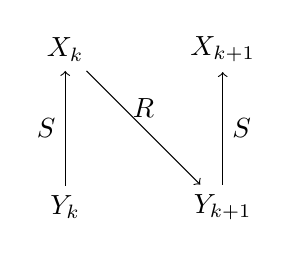
\begin{tikzpicture}[ node  distance=2cm]
\node(a){$X_k$};
\node(b)[below of =a]{$Y_k$};
\node(c)[right of =a]{$X_{k+1}$};
\node(d)[below of =c]{$Y_{k+1}$};

\draw[->](b)--(a)node[pos=0.5, left]{$S$};
\draw[->](a)--(d)node[pos=0.5, above]{$R$};
\draw[->](d)--(c)node[pos=0.5, right]{$S$};
\end{tikzpicture}
\caption{In this example, sampling from $R$ and $S$ is feasible.}
 \label{fig:DA:Gibbs}
\end{figure}

It turns out that $\sequence{X}[k][\nset]$ is a Markov chain with Markov kernel $RS$ and $\pi$ is
reversible wrt $RS$.
\begin{lemma}
  \label{lem:da:revers}
  The distribution $\pi$ is reversible with respect to the kernel $RS$.
\end{lemma}


\begin{proof}
We must prove that the measure $\pi\otimes RS$ on $\Xset^2$ is
  symmetric. For $A,B\in\Xsigma$, applying (\ref{eq:pipipi}), we have
  \begin{align*}
    \pi & \otimes RS(A\times B) \\
        & = \int_{\Xset\times\Yset} \pi(\rmd x) R(x,\rmd y) \indi{A}(x)  S(y,B)
          = \int_{\Xset\times\Yset}  \indi{A}(x)  S(y,B) \pi^*(\rmd x \rmd y) \\
        & = \int_{\Xset\times\Yset}  \indi{A}(x)  S(y,B) S(y,\rmd x) \tilde\pi(\rmd y)
          = \int_{\Yset}    S(y,A) S(y,B) \tilde\pi(\rmd y) \eqsp .
  \end{align*}
  This proves that $\pi\otimes RS$ is symmetric.
\end{proof}
%
Assume now that sampling from $R$ or $S$ is infeasible. In this case, we consider two instrumental
kernels $Q$ on $(\Xset \times \Yset) \times \Ysigma$ and $T$ on
$(\Xset \times \Yset) \times \Xsigma$ which will be used to propose successive candidates for
$Y_{k+1}$ and $X_{k+1}$. For simplicity, assume that $R(x,\rmd y')$ and $Q(x,y;\rmd y')$
(resp. $S(y',\rmd x')$ and $T(x,y';\rmd x')$) are dominated by the same measure and call $r$ and $q$
(resp. $s$ and $t$) the associated transition densities. We assume that $r$ and $s$ are known up to
a normalizing constant. Define the Markov chain \dsequence{X}{Y}[k][\nset] as follows. Given
$(X_k,Y_k)=(x,y)$,
\begin{enumerate}[({DA}1)]
\item \label{item:da:first} draw a candidate $\tilde{Y}_{k+1}$ according to the distribution
  $Q(x,y;\cdot)$ and accept $Y_{k+1}=\tilde{Y}_{k+1}$ with probability $\alpha(x,y,\tilde{Y}_{k+1})$
  defined by
  \begin{align*}
    \alpha(x,y,y') = \frac{r(x,y') q(x,y';y)}{r(x,y)q(x,y;y')} \wedge 1 \eqsp ;
  \end{align*}
  otherwise, set $Y_{k+1}=Y_k$; the Markov kernel on $\Xset\times\Yset\times\Ysigma$ associated to
  this transition is denoted by $K_1$;
\item \label{item:da:second} draw then a candidate $\tilde{X}_{k+1}$ according to the distribution
  $T(x,Y_{k+1};\cdot)$ and accept $X_{k+1}=\tilde{X}_{k+1}$ with probability
  $\beta(x,Y_{k+1},\tilde{X}_{k+1})$ defined by
  \begin{align*}
    \beta(x,y,x') = \frac{s(y,x') t(x',y;x)}{s(y,x)t(x,y;x')} \wedge 1 \eqsp ;
  \end{align*}
  otherwise, set $X_{k+1}=X_k$; the Markov kernel on $\Xset\times\Yset\times\Xsigma$ associated to
  this transition is denoted by $K_2$.
\end{enumerate}
For $i=1,2$, let $K_i^*$ be the kernels associated to $K_1$ and $K_2$ as follows: for $x\in\Xset$,
$y\in\Yset$, $A\in\Xsigma$ and $B\in\Ysigma$,
\begin{align}
  K_1^*(x,y;A\times B) & = \indi{A}(x) K_1(x,y;B) \eqsp . \label{eq:def-K1star} \\
  K_2^*(x,y;A\times B) & = \indi{B}(y) K_2(x,y;A) \eqsp . \label{eq:def-K2star}
\end{align}
%
Then, the kernel of the chain $\dsequence{X}{Y}[n][\nset]$ is $K=K_1^*K_2^*$.  The process
$\sequence{X}[n][\nset]$ is in general not a Markov chain since the distribution of $X_{k+1}$
conditionally on $(X_k,Y_k)$ depends on $(X_k,Y_k)$ and on $X_k$ only, except in some special cases.
Obviously, this construction includes the previous one where sampling from $R$ and $S$ was
feasible. Indeed, if $Q(x,y;\cdot)=R(x,\cdot)$ and $T(x,y;\cdot)=S(x,\cdot)$, then the acceptance
probabilities $\alpha$ and $\beta$ defined above simplify to one, the candidates are always accepted
and we are back to the previous algorithm.


\begin{framed}
\begin{proposition}
  \label{prop:DA}
  The extended target distribution $\pi^*$ is reversible wrt the kernels $K_1^*$ and $K_2^*$ and
  invariant with respect to~$K$.
\end{proposition}
\end{framed}

\begin{proof}
  The reversibility of $\pi^*$ with respect to $K_1^*$ and $K_2^*$ implies its invariance and
  consequently its invariance with respect to the product $K=K_1^*K_2^*$. Let us prove the
  reversibility of $\pi^*$ with respect to $K_1^*$. For each $x\in\Xset$, the kernel
  $K_1(x,\cdot;\cdot)$ on $\Yset\times\Ysigma$ is the kernel of a Metropolis-Hastings algorithm with
  target density $r(x,\cdot)$, proposal kernel density $q(x,\cdot;\cdot)$ and acceptation
  probability $\alpha(x,\cdot,\cdot)$. It implies that the
  distribution $R(x,\cdot)$ is reversible with respect to the kernel $K_1(x,\cdot;\cdot)$. Applying
  the definition~(\ref{eq:def-K1star}) of~$K_1^*$ and $\pi^*=\pi\otimes R$ yields, for
  $A,C\in\Xsigma$ and $B,D\in\Ysigma$,
  \begin{align*}
    \pi^* \otimes K_1^*(A\times B\times C\times D)
    & = \iint_{A\times B} \pi(\rmd x\rmd y) K_1^*(x,y;C\times D)  \\
    & = \iint_{A\times B} \pi(\rmd x) R(x,\rmd y) \indi{C}(x) K_1(x,y,D) \\
    & = \int_{A\cap C} \pi(\rmd x) [R(x,\cdot) \otimes K_1(x,\cdot;\cdot)] (B\times D) \eqsp .
  \end{align*}
  We have seen that for each $x\in\Xset$, the measure $R(x,\cdot) \otimes K_1(x,\cdot;\cdot) $ is
  symmetric, thus $\pi^* \otimes K^*$ is also symmetric. The reversibility of $\pi^*$ with respect
  to $K_2^*$ is proved similarly.
\end{proof}

\begin{example} [The slice sampler]
  \label{ex:slice:one} \index{slice sampler}
Set $\Xset=\rset^d$ and $\Xsigma=\mathcal{B}(\Xset)$. Let $\mu$ be a $\sigma$-finite measure on
$(\Xset,\Xsigma)$ and let $h$ be the density with respect to $\mu$ of the target distribution. We
assume that for all $x \in \Xset$,
%
\begin{align*}
  h(x) = C\prod_{i=0}^k f_i(x) \eqsp ,
\end{align*}
where $C$ is a constant (which is not necessarily known) and $f_i: \rset^d \to \rset^+$ are
nonnegative measurable functions.  For $y =(y_1,\ldots,y_k)\in {\rset^+}^k$, define
\begin{align*}
  L(y) = \set{x\in \rset^d}{f_i(x)\geq y_i\,, \eqsp i=1,\ldots, k} \eqsp .
\end{align*}
%
The  $f_0$-slice-sampler algorithm proceeds as follows:
\begin{itemize}
\item given $X_n$, draw independently a $k$-tuple $Y_{n+1}=(Y_{n+1,1}, \dots, Y_{n+1,k})$ of
  independent random variables such that $Y_{n+1,i} \sim \mathrm{Unif}(0,f_i(X_n))$, $i=1,\dots,k$.
\item sample $X_{n+1}$ from the % truncated probability %%% c'est quoi???
  distribution with density proportional to $f_0\indi{L(Y_{n+1})}$.
\end{itemize}
Set $\Yset=(\rset^+)^k$ and for $(x,y) \in \Xset \times \Yset$,
\begin{align*}
  h^*(x,y)=C f_0(x) \indi{L(y)}(x) = h(x) \prod_{i=1}^k
  \frac{\indi{[0,f_i(x)]}(y_i)}{f_i(x)} \eqsp .
\end{align*}
Let $\pi^*$ be the probability measure with density $h^*$ with respect to Lebesgue's measure on
$\Xset\times\Yset$. Then $\int_{\Yset}h^*(x,y)\rmd y = h(x)$ i.e. $\pi$ is the first marginal of
$\pi^*$. Let $R$ be the kernel on $\Xset\times\Ysigma$ with kernel denisty $r$ defined by
\begin{align*}
  r(x,y) = \frac{h^*(x,y)}{h(x)} \indi{h(x)>0} \eqsp .
\end{align*}
Then $\pi^* = \pi\otimes R$. Define the distribution $\tilde\pi=\pi R$, its density $\tilde{h}(y) =
\int_\Xset h^*(u,y) \rmd u$ and the kernel $S$ on $\Yset\times\Xsigma$ with density $s$ by
\begin{align*}
  s(y,x) = \frac{h^*(x,y)}{\tilde{h}(y)} \indi{\tilde{h}(y)>0} \eqsp .
\end{align*}
If $(X,Y)$ is a vector with distribution $\pi^*$, then $S(y,\cdot)$ is the conditional distribution
of $X$ given $Y=y$ and the Markov kernel of the chain $\sequence{X}[n][\nset]$ is $RS$ and
\Lemref{da:revers} can be applied to prove that $\pi$ is reversible, hence invariant, with respect
to $RS$.
\end{example}




\subsection{Two-stage Gibbs sampler}
\label{sec:two-stages-gibbs}
\index{Gibbs sampler}
The Gibbs sampler is a simple method which decomposes a complex multidimensional distribution into a
collection of smaller dimensional ones.  Let $(\Xset,\Xsigma)$ and $(\Yset,\Ysigma)$ be complete
separable metric spaces endowed with their Borel $\sigma$-fields.  To construct the Markov chain
$\dsequence{X}{Y}[n][\nset]$ with $\pi^*$ as an invariant probability, we proceed exactly as in
data-augmentation algorithms. Assume that $\pi^*$ may be written as
\begin{equation}
  \label{eq:definition-pistar}
  \pi^*(\rmd x\rmd y) = \pi(\rmd x) R(x,\rmd y) = \tilde{\pi}(\rmd y)   S(y,\rmd x)
\end{equation}
where $\pi$ and $\tilde \pi$ are probability measures on $\Xset$ and $\Yset$ respectively and $R$
and $S$ are kernels on $\Xset \times \Ysigma$ and $\Yset \times \Xsigma$ respectively.


\subsubsection*{The deterministic updating (two-stage) Gibbs (DUGS) sampler}
\index{DUGS}
When sampling from $R$ and $S$ is feasible, the DUGS sampler proceeds as follows: given $(X_k,Y_k)$,
\begin{enumerate}[({DUGS}1)]
\item \label{item:gibbs-1} sample $Y_{k+1}$ from $R(X_k,\cdot)$,
\item \label{item:gibbs-2} sample $X_{k+1}$ from $S(Y_{k+1},\cdot)$.
\end{enumerate}
For both the Data Augmentation algorithms and the two-stage Gibbs sampler we consider a distribution
$\pi^*$ on the product space $\Xset \times \Yset$. In the former case, the distribution of interest
is a marginal distribution of $\pi^*$ and in the latter case the target
distribution is $\pi^*$ itself.

We may associate to each update \ref{item:gibbs-1}-\ref{item:gibbs-2} of the algorithm a
transition kernel on $(\Xset \times \Yset) \times (\Xsigma \otimes \Ysigma)$ defined for
$(x,y) \in \Xset \times \Yset$ and $A\times B \in \Xsigma \otimes \Ysigma$ by
\begin{align}
  \label{eq:definition-R^*}
  R^*(x,y;A\times B)  & = \indi{A}(x)R(x,B) \eqsp , \\
  \label{eq:definition-S^*}
  S^*(x,y;A \times B) & = \indi{B}(y)S(y,A) \eqsp .
\end{align}
% \begin{align}
%   \label{eq:definition-R^*}
%   R^*(x,y;C) &= \iint \delta_x(\rmd x') R(x',\rmd y') \1_C(x',y') \\
%   \label{eq:definition-S^*}
%   S^*(x,y;C) &= \iint \delta_y(\rmd y') S(y, \rmd x') \1_C(x',y') \eqsp.
% \end{align}
The transition kernel of the DUGS is then given by
\begin{equation}
  \label{eq:kernel:DUGS}
  P_{\mathrm{DUGS}} = R^* \, S^* \eqsp.
\end{equation}
Note that for $A\times B \in \Xsigma \otimes \Ysigma$,
\begin{align}
  P_{\mathrm{DUGS}}(x,y;A\times B)
  & = \iint_{\Xset\times\Yset}  R^*(x,y;\rmd x' \rmd y') S^*(x',y'; A \times B) \nonumber \\
  & = \iint_{\Xset\times\Yset}   R(x,\rmd y') \indi{B}(y')S(y',A)  \nonumber \\
  & = \int_B R(x,\rmd y') S(y',A) = R \otimes S (x,B\times A) \eqsp . \label{eq:identity-PDUGS}
  % \\
  % & = \idotsint \delta_x(\rmd x') R(x,\rmd y') \delta_{y'}(\rmd y'') S(y',\rmd x'') \1_C(x'',y'')
  % \\
  % & = \iint R(x,\rmd y') S(y', \rmd x'') \1_C(x'',y')= R \otimes S(x,C) \eqsp.
\end{align}

As a consequence of \Propref{DA}, we obtain the invariance of $\pi^*$.
\begin{lemma}
  \label{lem:gibbs-reversibility-individual}
  The distribution $\pi^*$ is reversible with respect to the kernels $R^*$ and $S^*$ and invariant
  with respect to $P_{\mathrm{DUGS}}$.
\end{lemma}





\subsubsection*{The Random Scan Gibbs sampler (RSGS)}
\index{random scan} \index{rsgs}
At each iteration, the RSGS algorithm consists in updating one component chosen at random. It
proceeds as follows: given $(X_k,Y_k)$,
\begin{enumerate}[label=(RSGS\arabic*)]
\item \label{item:rsgs-gibbs-0} sample a Bernoulli random variable $B_{k+1}$ with probability of
  success $1/2$.
\item \label{item:rsgs-gibbs-1} If $B_{k+1}= 0$, then sample $Y_{k+1}$ from $R(X_k,\cdot)$ else
  sample $X_{k+1}$ from $S(Y_{k+1},\cdot)$.
\end{enumerate}
The transition kernel of the RSGS algorithm can be written
\begin{equation}
  \label{eq:kernel:RSGS}
  P_{\mathrm{RSGS}}= \frac{1}{2} R^* + \frac{1}{2} S^* \eqsp.
\end{equation}
\Lemref{gibbs-reversibility-individual} implies that $P_{\mathrm{RSGS}}$ is reversible wrt
$\pi^*$ and therefore  $\pi^*$ is invariant for $P_{\mathrm{RSGS}}$.

If sampling from $R$ or $S$ is infeasible, the Gibbs transitions can be replaced by a
Metropolis-Hastings algorithm on each component as in the case of the DUGS algorithm. The agorithm
is then called the Two-Stage Metropolis-within-Gibbs algorithm.


\section{After studying this chapter...}
\begin{center}
\shadowbox{\begin{minipage}{0.9\textwidth}
\begin{enumerate}[a)]
\item I can explain Pseudo marginal algorithm and I can justify why it is correct on a blackboard.
\item I understand understand the notions of deterministic moves and the requirements linked with MH with deterministic moves (involution, volume-preserving and invariant level sets), so I understand all about Hamiltonian MC.
\item I know and understand the Gibbs moves.
\item I am able to implement these variants of MH, pseudo marginal algorithms, Leapfrog HMC...
\end{enumerate}
\end{minipage}
}
\end{center}


\newpage
\section*{Highlights}

\begin{subappendices}

\section{William Rowan Hamilton (source: wikipedia).}

\begin{wrapfigure}{L}{0.25\textwidth} \centering

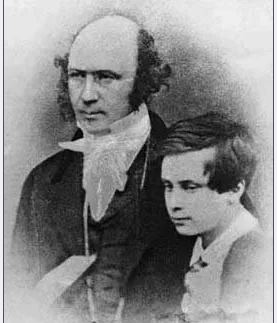
\includegraphics[scale=0.45]{hamilton}

\end{wrapfigure}

Sir William Rowan Hamilton MRIA (3 August 1805 - 2 September 1865) was an Irish mathematician, Andrews Professor of Astronomy at Trinity College Dublin, and Royal Astronomer of Ireland. He worked in both pure mathematics and mathematics for physics. He made important contributions to optics, classical mechanics and algebra. Although Hamilton was not a physicist, he regarded himself as a pure mathematician, his work was of major importance to physics, particularly his reformulation of Newtonian mechanics, now called Hamiltonian mechanics. This work has proven central to the modern study of classical field theories such as electromagnetism, and to the development of quantum mechanics. In pure mathematics, he is best known as the inventor of quaternions.


William Rowan Hamilton's scientific career included the study of geometrical optics, classical mechanics, adaptation of dynamic methods in optical systems, applying quaternion and vector methods to problems in mechanics and in geometry, development of theories of conjugate algebraic couple functions (in which complex numbers are constructed as ordered pairs of real numbers), solvability of polynomial equations and general quintic polynomial solvable by radicals, the analysis on Fluctuating Functions (and the ideas from Fourier analysis), linear operators on quaternions and proving a result for linear operators on the space of quaternions (which is a special case of the general theorem which today is known as the Cayley-Hamilton theorem). Hamilton also invented "icosian calculus", which he used to investigate closed edge paths on a dodecahedron that visit each vertex exactly once.
\end{subappendices}


\chapter{Target distributions and alternative methods}
So far, in MCMC methods, a target distribution $\pi$ is given and we have shown some generic ways of constructing a process $(X_k)_{k\in\nset}$ that targets $\pi$ in some sense to be defined: sometimes $(X_k)_{k\in\nset}$ is itself a Markov chain with invariant probatility measure $\pi$, sometimes, $(X_k)_{k\in\nset}$ is the first component process of an extended Markov chain that targets an extended distribution where the marginal distribution on the first component is $\pi$.


\section{Target distributions}
We first introduce two contexts where target distributions are at stake. One is linked with Bayesian inference. In such a case, the target distribution is the posterior distribution of the parameter given all the data. Another one is linked with partially observed models. In such a case, the target distribution  might be the distribution of the unobserved variables given the data.

\subsection{Bayesian inference}
\index{bayeasian inference}
In  Bayesian inference, prior belief  is combined with
data to obtain posterior distributions on which statistical inference is based.
%Although we focus primarily on  likelihood based inference in this text,
%it is also worthwhile to consider Bayesian  inference  for some problems.
Except for some simple cases, Bayesian inference can be computationally
intensive and may rely on  computational techniques.

The basic idea in Bayesian analysis is that a parameter vector,
say $ \theta \in \Theta$, is unknown to a researcher, so a \emph{prior} distribution,
$\pi_0( \theta)\lambda(\rmd \theta)$, is put on the parameter vector.  The researcher also
proposes a model or likelihood, $\dens[][]{ y_{1:n} \mid \theta}$, that describes
how the data $Y=y_{1:n}$ depend on the parameter vector.
Inference about $ \theta$ is then based on the \emph{posterior}
distribution, which is obtained via Bayes's theorem,
\begin{equation} \label{eq:target:bayes}
\pi(\theta)=\dens[][]{\theta \bigm| Y=y_{1:n}}=\frac{\pi_0( \theta) \dens[][]{ y_{1:n} \mid \theta}}{\int \pi_0( \theta) \dens[][]{ y_{1:n} \mid \theta} \lambda(\rmd \theta)}.
\end{equation}
  In some simple cases, the prior  and
the likelihood are \emph{conjugate}  distributions that may be combined easily.
For example, in $n$ fixed repeated (iid) Bernoulli experiments with probability of success $\theta$,
a \emph{Beta-Binomial} conjugate pair is taken.  In this case the prior is
Beta($a,b$):
$\pi_0(\theta) \propto \theta^{a} (1-\theta)^{b}$; the values $a,b > -1$  are called
hyperparameters. The likelihood in this example is
Binomial$(n,\theta)$:
$\dens[][]{ y \mid \theta} \propto \theta^y (1-\theta)^{n-y}$, from which
we easily deduce that the
posterior is also Beta,
$\pi ( \theta \bigm| Y ) \propto \theta^{y+a}(1-\theta)^{n+b-y }
$, and from which inference may easily be achieved.
In more complex experiments, the posterior distribution is often difficult to obtain by direct calculation,
so MCMC techniques are employed (note that in \eqref{eq:target:bayes}, the numerator is usually known and explicit while, due to the integral, the denominator is a multiplicative unknown constant).  The main idea is that we may not be able to
explicitly display the posterior, but we may be able to simulate from
the posterior.

%Nevertheless, even when $\theta$ is in a small dimension space, the numerical calculation of $p(y_{1:n}|\theta)$ may be hard to obtain  precisely due to the fact that $n$ is large. For example, in the case of iid random variables, $p(y_{1:n}|\theta)$ is
%a large product
%$\prod_{i=1}^n p(y_i|\theta)$  (since $n$ is the number of the observations).

\subsection{Models with Latent variables}
In some situations, observations are partial and unfortunately, do not contain some variables of interest. In such a case, given a modelization of the process generating the data, one might be interested into reconstructing the distribution of the missing variables given the data. This will be our target distribution. Let us be more specific with the example of Hidden Markov Models (HMM).
\index{hidden Markov models} \index{latent variables}

Such a model is defined by a bivariate Markov chain $(Z_k)_{k\in\nset}=(X_k,Y_k)_{k\in\nset}$ on $\Xset\times\Yset$ where $(\Xset,\Xsigma)$ and $(\Yset,\Ysigma)$ are two measurable spaces, and where the transition is given by:
\begin{align*}
X_k|_{Z_{0:k-1}} \sim Q(X_{k-1},\cdot)\\
Y_k|_{X_k,Z_{0:k-1}} \sim G(X_k,\cdot)
\end{align*}
Here, $Q$ denotes a Markov kernel on $\Xset \times \Xsigma$ while $G$ is a Markov kernel on $\Xset \times \Ysigma$.


\begin{figure}[!h]
\begin{center}
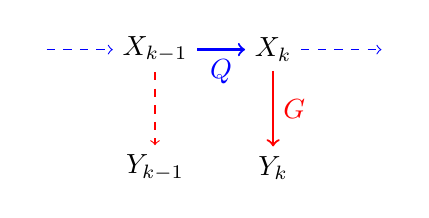
\begin{tikzpicture}[node  distance=1.5cm]
\node(a){$X_{k-1}$};
\node(b)[right of =a]{$X_{k}$};
\node(c)[below of =b]{$Y_{k}$};
\node(d)[left of =c]{$Y_{k-1}$};
\node(e)[right of =b]{};
\node(f)[left of =a]{};

\draw[->, blue,thick](a)--(b)node[pos=0.5, below]{$Q$};
\draw[->, red,thick](b)--(c)node[pos=0.5, right]{$G$};
\draw[->, dashed, blue](b)--(e);
\draw[->, dashed, red](a)--(d);
\draw[->, dashed, blue](f)--(a);
\end{tikzpicture}
\end{center}

\caption{A hidden Markov model}
\label{hmm}
\end{figure}
In such a model, only the $Y$'s component is observed and inference must be driven on the basis of $(Y_{1:n})$ only.
In a fully dominated model, we assume that $Q(x,\rmd x')=q(x,x') \lambda(\rmd x')$ and $G(x,\rmd y)=g(x,y) \nu(\rmd y)$ where $\lambda$ and $\nu$ are $\sigma$-finite dominating measures on $(\Xset,\Xsigma)$, and $(\Yset, \Ysigma)$ respectively. In such a case, assuming that $X_0=x_0$ is given, one might be interested in the law of the missing variables $X_{1:n}$ given the observations $Y_{1:n}$, so that the target density will be:
$$
\pi(x_{1:n})=\frac{\prod_{i=1}^{n} q(x_{i-1},x_i)g(x_i,y_i)}{\idotsint_{\Xset^n} \prod_{i=1}^{n} q(x_{i-1},x_i)g(x_i,y_i) \lambda(\rmd x_i)}
$$
Once again the denominator is, due to the integral, an unknown multiplicative factor, whereas the numerator is explicit and we are therefore in a context where MCMC methods can be applied. Nevertheless, in this example, the number of hidden variables is $n$, which can be very large and the target distribution is thus associated to a very high dimensional space, $\Xset^n$, so that we have to be very careful when applying these methods.
\section{Other approximation methods}
In computational statistics, when it comes to approaching a target law in a very large space,
classical techniques using Markov chains admitting "exactly" this target law
for invariant distribution may suffer from a slow exploration of the state space. In a high dimensional framework, the candidate is often proposed in an uninformative region and it is likely that it is refused, leading the Markov chain to remain stuck at the same place a certain amount of time.

Some other approximation techniques do not even try to construct random variables with distribution close to $\pi$. We will briefly introduce two approximation techniques: sequential Monte Carlo methods and Variational Inference.

\subsection{Sequential Monte Carlo methods}
\index{sequential Monte Carlo}
We briefly explain basic ideas of Sequential Monte Carlo methods, without proving anything.
The rough idea of sequential Monte Carlo methods for targetting $\pi$ is to find intermediate target distributions $\pi_1\rightarrow \pi_2\rightarrow,\ldots,\rightarrow \pi_T=\pi$ and to construct, sequentially, Monte Carlo approximations of $\pi_i$.




This is actually based on importance sampling and we first recall it here. If $\pi$ and $g$ are densities wrt to the same dominating measure, and assuming that $g(x)=0$ implies $\pi(x)=0$, then we can approximate $\pi(h)$ with $N^{-1}\sum_{k=1}^N \frac{\pi(X_k)}{g(X_k)} h(X_k)$ where $(X_k)_{k\in[1:N]} \iid g$. Since $\pi$ is typically known only up to a multiplicative factor, the quantity $n^{-1}\sum_{k=1}^N \frac{\pi(X_k)}{g(X_k)} h(X_k)$ is not explicit due to this multiplicative factor and we typically choose instead:
$$
\pi(h) =\frac{\pi(h)}{\pi(1)}\approx \frac{n^{-1}\sum_{k=1}^N \frac{\pi(X_k)}{g(X_k)} h(X_k)}{N^{-1}\sum_{\ell=1}^n \frac{\pi(X_\ell)}{g(X_\ell)}}=\sum_{k=1}^N \lr{\frac{ \omega^k}{\sum_{\ell=1}^N \omega^\ell}}  h(X_k)=\sum_{k=1}^N \bar\omega^k  h(X_k)
$$
where $\omega^k=\pi(X_k)/g(X_k)$ and $\bar \omega^k=\omega^k/(\sum_{\ell=1}^{k} \omega^\ell)$. Now the rhs can be calculated even if $\pi$ is known only up to a multiplicative factor since $\bar \omega^k$ is a ratio where $\pi$ is involved (both in the numerator and the denominator).

Thus, $\pi(h)$ is approximated using a population of "particles" $\{(X_k,\omega^k)\}_{k\in[1:N]}$ (we mean by particle a "support" point $X_k$ and an associated weight $\omega^k$). Note that a weight is usually unnormalized but when considering the approximation, we use the normalized weights: $\omega^k/(\sum_{\ell=1}^{k} \omega^\ell)$.

Of course, if all the $X_k$ were iid from $\pi$ directly, all the associated weights would be equal. So here, by allowing different weights, we are more flexible. Still if the weights are too different, this is not satisfactory because only a few particles contain all the information. In that case, we prefer to resample inside the population. Let us be more specific.

\subsubsection{Resampling step}
\index{resampling}
Assume that $\{(X_k,\omega^k)\}_{k\in[1:N]}$ targets $\pi_0(h)$. Define $\bar \omega^k=\omega^k/(\sum_{\ell=1}^{k} \omega^\ell)$.

An example of resampling step is
$$
\mbox{For $k\in[1:n]$, choose independently}\quad \tilde X_k=\begin{cases}
X_1& \mbox{wp} \ \bar \omega^1\\
\ldots&\\
X_N & \mbox{wp} \ \bar \omega^N
\end{cases}
$$
Then $\{(\tilde X_k,1)\}_{k\in[1:N]}$ still targets $\pi_0(h)$. The target distribution is not changed but now, all the weights are equal. Informative particles (ie with high weights) are likely to be replicated after resampling while noninformative are likely to disappear (because they were not chosen). Support points are changed but still within the initial pool of support points.

\subsubsection{Exploration step}
\index{exploration}
Assume that $\{(X_k,\omega^k)\}_{k\in[1:N]}$ targets $\pi_0(h)$ and that
\begin{equation} \label{eq:explor}
\pi_1(y)=\int_\Xset \pi_0(\rmd x) q(x,y)\eqsp,
\end{equation}
where $q$ is a kernel density. An example of exploration step is
$$
\mbox{For $k\in[1:n]$, draw independently}\quad \tilde X_k\sim r(X_k,\cdot)
$$
where $r$ is a kernel density (that can be easily simulated).
Then, $\lrcb{(\tilde X_k,\omega^k \times \frac{q(X_k,\tilde X_k)}{r(X_k,\tilde X_k)}}_{k\in[1:N]}$ targets $\pi_1(h)$.
Here, support points are moved and weights are updated by a multiplicative factor (except when $r=q$, in which case, support points are moved but the associated weights do not need to be updated  since $ \frac{q(X_k,\tilde X_k)}{r(X_k,\tilde X_k)}=1$).
\subsubsection{Reweighting step}
\index{reweighting}
Assume that $\{(X_k,\omega^k)\}_{k\in[1:N]}$ targets $\pi_0(h)$ and that
\begin{equation} \label{eq:resamp}
\pi_1(x)=\frac{ \pi_0(x) g(x) }{\int_\Xset \pi_0(\rmd u) g(u) }
\end{equation}
where $g$ is a nonnegative function. Then,  $\lrcb{(X_k,\omega^k g(X_k) }_{k\in[1:N]}$ targets $\pi_1(h)$. Here, support points are unchanged but weights are updated.

Finally, when choosing the intermediate target distributions $\pi_1\rightarrow \pi_2\rightarrow,\ldots,\rightarrow \pi_T=\pi$, we must check that each step $\pi_i \rightarrow \pi_{i+1}$ corresponds either to \eqref{eq:explor} or \eqref{eq:resamp} so that we can let evolve a population of particles through exploration, and reweighting steps. Resampling can always be performed when weights are too different and this is often measured when the Effective Sample Size (which is a real number between 1 and $N$), $\widehat{ESS}=\frac{1}{\sum_{k=1}^N (\bar \omega^k)^2}$, falls below a certain arbitrary threshold.
\subsection{Variational inference}
\index{variational inference}
Variational Inference is a technique derived from the
 {\em Machine Learning} community whose principle is to approach the target density through various optimization techniques. The principle consists in giving up aiming exactly at the target law, but instead, we have at hand a sufficiently rich family of laws (that can be easily simulated) and the idea is then to select a member of this family close to the target in the sense of a certain divergence through optimization procedures. Variational inference has been successfully used in many applications and seems to be faster and more efficient to explore large spaces compared to classical Monte Carlo Markov chain methods. The proximity is often measured in terms of Kullback divergence or even more recently in terms of $f$-divergence. Although these techniques are extremely powerful and popular in practice, some statistical properties of these methods are still largely unknown.

\subsubsection{$\alpha$-divergence and the ELBO}
\index{$\alpha$-divergence}
Letting $f_\alpha$ be the convex function on $(0, +\infty)$ defined by $f_0(u) = -\log(u)$, $f_1(u) = u\log(u)$ and $f_\alpha(u) = \frac{1}{\alpha(\alpha-1)} \left[  u^\alpha -1 \right]$ for all $\alpha \in \rset \setminus \lrcb{0,1}$, the $\alpha$-divergence for all $\alpha \in \rset$ is defined by
\begin{align}\label{eq:gen:div}
D_\alpha(\mathbb{P}\|\mathbb{Q}) = \int_\Xset f_\alpha\left(\frac{q(x)}{p(x)} \right)p(x) \lambda(\rmd x) \eqsp,
\end{align}
where $\mathbb{P}(\rmd x)=p(x)\lambda(\rmd x)$ and $\mathbb{Q}(\rmd x)=q(x) \lambda(\rmd x)$. Of course, it is non-negative and null if $\mathbb{P}=\mathbb{Q}$ but there is no triangular inequality and therefore, it is not a distance.



\newcommand{\argmin}{\mathrm{argmin}}
In Variational Inference (also called VI), we want to approximate $\pi$ by selecting the best candidate among a family of densities
$$
\set{x\mapsto p_\theta(x)}{\theta\in\Theta}
$$
with respect to the $\alpha$-divergence. In other words, we want to solve
$$
\argmin_{\theta\in\Theta} D_\alpha(\pi \| p_\theta)= \argmin_{\theta\in\Theta} \int_{\Xset} f_\alpha\lr{\frac{p_\theta(x)}{\pi(x)}} \pi(x) \lambda(\rmd x)
$$
Recalling that $\pi$ is known only up to multiplicative constant, we must check if the minimization of $\int_{\Xset} f_\alpha\lr{\frac{p_\theta(x)}{\pi(x)}} \pi(x) \lambda(\rmd x)$ can be equivalent to the minimization of another functional which will be more explicit. Write $\pi(x)=\tilde \pi(x)/C$ where $\tilde \pi(x)$ is explicit and $C=\int_\Xset \tilde \pi(x)\lambda(\rmd x)$ is an "unexplicit" constant. Take for example: $\alpha=1$. Then,
$$
D_1(\pi \| p_\theta)= \int_{\Xset} \log\lr{\frac{p_\theta(x)}{\pi(x)}} p_\theta(x) \lambda(\rmd x)=-\underbrace{\int_{\Xset} \log\lr{\frac{\tilde \pi(x)}{p_\theta(x)}} p_\theta(x) \lambda(\rmd x)}_{ELBO} + \log C
$$
\index{ELBO}
In this litterature, $\int_{\Xset} \log\lr{\frac{\tilde \pi(x)}{p_\theta(x)}} p_\theta(x) \lambda(\rmd x)$ is called the ELBO (Evidence Lower Bound) and maximizing the ELBO wrt $\theta$ is equivalent to minimizing $ D_1(\pi \| p_\theta)$ wrt $\theta$. Note that
since $D_1(\pi \| p_\theta)=-ELBO+ \log C$, we have
$$
ELBO \leq \log C=\log \int_\Xset \tilde \pi(x)\lambda(\rmd x)
$$
(Hence, the terminology "Evidence Lower Bound"). In the case where $\alpha \neq 1$, some equivalent of the ELBO can also be found. In VI, we are face to an optimisation problem (which is in general a non-convex problem) and we have to resort to all the tools linked with optimisation problems: various stochastic gradient descents and their variants...



\section{Approximate Bayesian computation}
Approximate Bayesian computation (ABC) is an alternative approach when computation of the posterior is challenging, either because the size of the data or the complexity of realistic models makes the calculation computationally intractable. ABC specifically provides a solution  when the likelihood $y\mapsto p(y|\theta)$ cannot be evaluated. A generic description of the original ABC algorithm requires (i) the introduction of statistics $S(y)\in\mathbb{R}^m$ where $m$ is usually sensibly smaller than the dimension of $y$ and (ii) a distance $\mathsf{d}$ on $\mathbb{R}^m\times \mathbb{R}^m$. Note that if no statistics can be widely defined $S$ can be the identity function. Then, the most direct ABC alforithm is described in Algorithm~\ref{alg:ABC}.

\medskip

\begin{algorithm}[H] \label{alg:ABC}
    \KwData{Observation $Y$, threshold $\varepsilon$, $N$}
    \KwResult{Samples approximately distributed according to $p(\cdot | Y)$.}
    \For {$i = 1 \to N$}{
        draw $\theta_i$ with prior distribution $\pi$\;
        draw $Y_i$ with distribution  $p(\cdot |\theta_i)$\;
}
Return all $\theta_i$ such that $\mathsf{d}(S(Y_i),S(Y))<\varepsilon$\;
\caption{ABC algorithm.}
\end{algorithm}

\medskip

When $S$ is the identity function, the random variables sampled by this  algorithm have distribution $\pi_{\varepsilon}(\cdot |Y)$ where
$$
\pi_{\varepsilon}(\theta|Y)\propto \int p(y|\theta)\pi(\theta) \mathds{1}_{A_{\varepsilon,Y}}(y)\rmd y\eqsp,
$$
with $A_{\varepsilon,Y} = \{y\eqsp;\mathsf{d}(y,Y)<\varepsilon\eqsp\}$. The intuitive idea behind this algorithm is that if  $\varepsilon \to 0$, $\pi_{\varepsilon}(\theta|Y) \to \pi(\theta|Y)$ and if $\varepsilon \to \infty$, $\pi_{\varepsilon}(\theta|Y) \to \pi(\theta)$. This initial version of the ABC approach raises many practical  issues among which an appropriate calibration of $\varepsilon$, the choice of statistics $S$, and the widespread inefficiency of sampling candidates according to the prior distribution $\pi$. In practice, the threshold $\varepsilon$ is usually determined as a quantile of the observed distance $(\mathsf{d}(S(Y_i),S(Y)))_{1\leqslant i \leqslant N}$ which allows to introduce Algorithm~\ref{alg:ABC:quant}.

\medskip

\begin{algorithm}[H] \label{alg:ABC:quant}
    \KwData{Observation $Y$, $N$, integer $M_N$}
    \KwResult{Samples approximately distributed according to $p(\cdot | Y)$.}
    \For {$i = 1 \to N$}{
        draw $\theta_i$ with prior distribution $\pi$\;
        draw $Y_i$ with distribution  $p(\cdot |\theta_i)$\;
}
Return all $\theta_i$ such that $S(Y_i)$ is in the set of $M_N$ nearest neighbors of $S(Y)$ with respect to distance $\mathsf{d}$\;
\caption{ABC algorithm with calibrated threshold.}
\end{algorithm}

\medskip

These two algorithms generate independent samples but do not build upon the accepted samples to propose new candidates in a more efficient way than using the prior distribution. This can be performed by considering  ABC within a MCMC algorithm. See the exercises for a proof that Algorithm~\ref{alg:ABC:MCMC} targets the correct posterior distribution.

\medskip

\begin{algorithm}[H] \label{alg:ABC:MCMC}
\KwData{Observation $Y$, $N$, threshold $\varepsilon$,  output $(\theta_0,Y_0)$ from a "standard" ABC.}
\KwResult{Samples approximately distributed according to $p(\cdot | Y)$.}
\For{$i=1$ to $N$}{
Sample $\widetilde \theta \sim q(\cdot |\theta_i)$\;
Sample $\widetilde Y \sim p(\cdot|\widetilde \theta)$ and compute $S(\widetilde Y)$\;
Compute $\alpha = 1\wedge \frac{\pi(\widetilde \theta) q(\theta_i|\widetilde \theta)}{\pi(\theta_i) q(\widetilde\theta| \theta_i)}\mathds{1}_{\mathsf{d}(S(\tilde Y),S(Y))<\varepsilon}$\;
Sample $U\sim U(0,1)$\;
\eIf{$U< \alpha$}{
Set $\theta_{i+1} = \widetilde \theta$ and $Y_{i+1} = \widetilde Y$\;
}{
$\theta_{i+1} = \theta_i$ and $Y_{i+1} = Y_i$\;
}
}\caption{ABC within MCMC}
\end{algorithm}


\section{After studying this chapter...}
\begin{center}
\shadowbox{\begin{minipage}{0.9\textwidth}
\begin{enumerate}[a)]
\item I understand what are the typical target distributions and that they can be of high dimensions.
\item I have notions other approximations methods.
\item I understand the basic ways of letting evolve a population of particles (exploration, reweighting, resampling) and the associated moves of the target distribution.
\item I understand the basics of variational inference.
\item I am ready (and eager) to work in practise on various MH algorithms or approximation methods.
\end{enumerate}
\end{minipage}
}
\end{center}


\section*{Highlights}

\begin{subappendices}

\section{Thomas Bayes (source: wikipedia).}

\begin{wrapfigure}{L}{0.28\textwidth} \centering

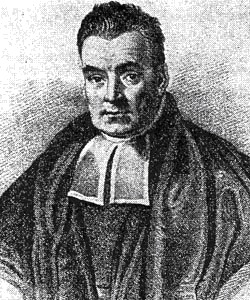
\includegraphics[scale=0.45]{bayes}

\end{wrapfigure}
Thomas Bayes (1701-1761) was an English statistician, philosopher and Presbyterian minister who is known for formulating a specific case of the theorem that bears his name: Bayes' theorem. Bayes never published what would become his most famous accomplishment; his notes were edited and published after his death by Richard Price.

Thomas Bayes was the son of London Presbyterian minister Joshua Bayes, and was possibly born in Hertfordshire. He came from a prominent nonconformist family from Sheffield. In 1719, he enrolled at the University of Edinburgh to study logic and theology. On his return around 1722, he assisted his father at the latter's chapel in London before moving to Tunbridge Wells, Kent, around 1734. There he was minister of the Mount Sion Chapel, until 1752.

He is known to have published two works in his lifetime, one theological and one mathematical:

\begin{itemize}
\item Divine Benevolence, or an Attempt to Prove That the Principal End of the Divine Providence and Government is the Happiness of His Creatures (1731)
\end{itemize}

\begin{itemize}
\item An Introduction to the Doctrine of Fluxions, and a Defence of the Mathematicians Against the Objections of the Author of The Analyst (published anonymously in 1736), in which he defended the logical foundation of Isaac Newton's calculus ("fluxions") against the criticism of George Berkeley, author of The Analyst
\end{itemize}

It is speculated that Bayes was elected as a Fellow of the Royal Society in 1742 on the strength of the Introduction to the Doctrine of Fluxions, as he is not known to have published any other mathematical works during his lifetime.

In his later years he took a deep interest in probability. Professor Stephen Stigler, historian of statistical science, thinks that Bayes became interested in the subject while reviewing a work written in 1755 by Thomas Simpson, but George Alfred Barnard thinks he learned mathematics and probability from a book by Abraham de Moivre. Others speculate he was motivated to rebut David Hume's argument against believing in miracles on the evidence of testimony in An Enquiry Concerning Human Understanding. His work and findings on probability theory were passed in manuscript form to his friend Richard Price after his death.


Monument to members of the Bayes and Cotton families, including Thomas Bayes and his father Joshua, in Bunhill Fields burial ground
By 1755 he was ill and by 1761 had died in Tunbridge Wells. He was buried in Bunhill Fields burial ground in Moorgate, London, where many nonconformists lie.
\end{subappendices}

\chapter{Illustrations, exercises, extensions}

\section{Illustrations}
A \textbf{``collaboratory'' Jupyter Notebook} that illustrates the
results of some exercises or some algorithms seen in the course is
at the disposal of the reader \href{https://colab.research.google.com/drive/1Ey5TNx-_74gPH0FG-rhXSuGGok0T10wS\#}{by following this link.}

\subsection{Illustrations of HMC}
Figure~\ref{fig:leapfrog} displays several trajectories of the leapfrog integrator when the target density is a Guassian distribution or a mixture of Gaussian distributions. Trajectories are initialized randomly and then the leapfrog integrator is run with step size $h= 0.01$.

\begin{figure} 
\label{fig:leapfrog}
\centering
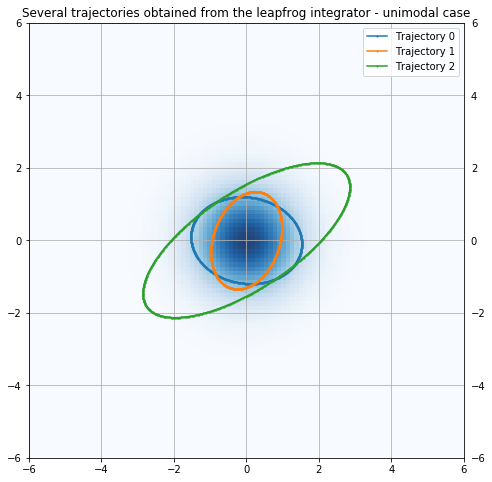
\includegraphics[scale=0.4]{leapfrog}
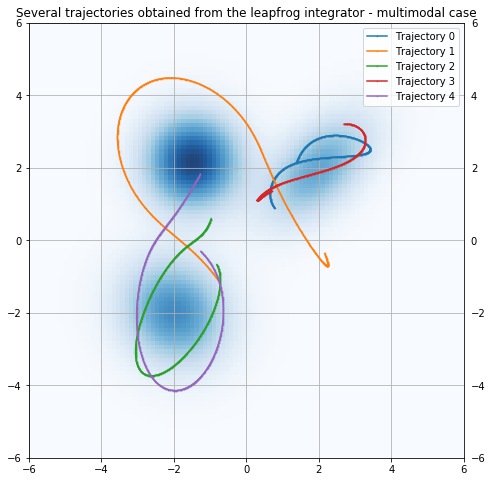
\includegraphics[scale=0.4]{leapfrog_mixture}
\end{figure}

Figure~\ref{fig:hmc:mixture} displays several trajectories of a HMC sampler with leapfrog integrators with various lengths when the target density a mixture of Gaussian distributions. This figure highlights the fact that the proposed moves provided by the leapfrog integrator allow to explore widely the space and to jump from a mode to another.

\begin{figure} 
\label{fig:hmc:mixture}
\centering
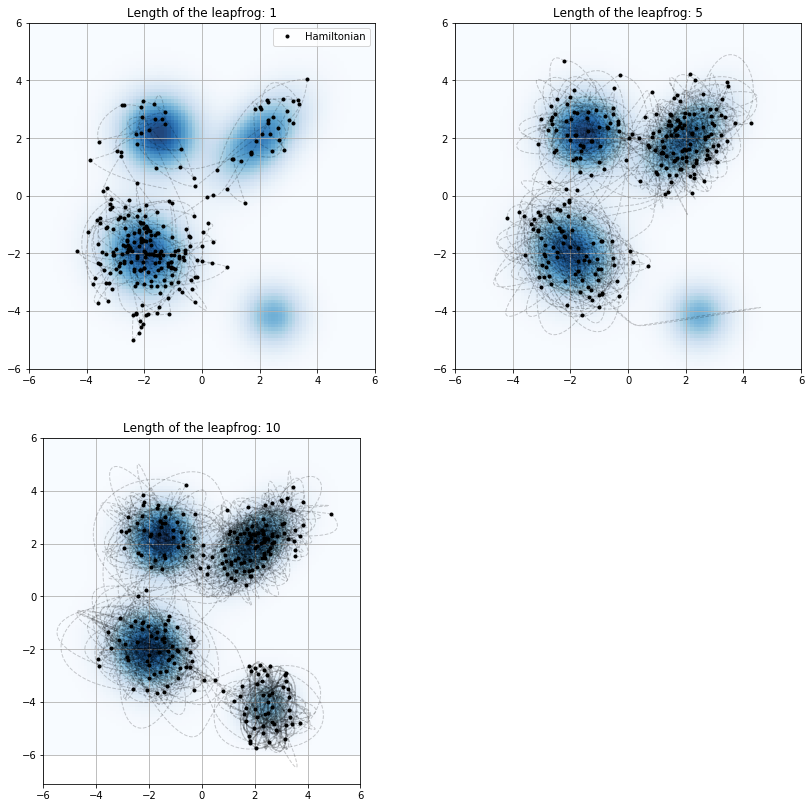
\includegraphics[scale=0.4]{HMC_mixture}
\end{figure}

\section{Exercises}
\begin{exercise}
\label{ex:arch}
Let
\[
X_{t}=\sigma_{t}Z_{t},\quad\sigma_{t}^2=\alpha_{0}+\alpha_{1}X_{t-1}^{2},\quad t\geq1
\]
where the coefficients $\alpha_{0},\alpha_{1}$ are positive and $\seq{Z_{t}}{t\in\nset}$
is an iid sequence of random variables such that $\PE[Z_{0}]=0$,
$\PE[Z_{0}^{2}]=1$, and $\seq{Z_{t}}{t\in\nset\ensuremath{}}$ is
independent of $X_{0}$
\begin{enumerate}
\item Assuming that $Z_{0}$ has the density $q$ wrt the Lebesgue measure,
show that $\seq{X_{t}}{t\in\nset}$ is a Markov chain with transition
density
\[
p(x,x')=\frac{1}{\sqrt{\alpha_{0}+\alpha_{1}x^{2}}}q\left(\frac{x'}{\sqrt{\alpha_{0}+\alpha_{1}x^{2}}}\right).
\]
\begin{answer}
Define $\mcf_t=\sigma(X_0,Z_{0:t})$ and note that $(X_t)$ is $(\mcf_t)$-adapted and check that
$$
\PE[h(X_{k+1})|\mcf_k]=\int_\Xset h(x) p(X_k,x)\rmd x
$$

\end{answer}

\end{enumerate}
\end{exercise}

\begin{exercise} \label{exo:solidarite}
Let $\mu\in\meas{1}(\Xset)$ and assume that for some function $h\in\funcset{}(\Xset)$, and some constant $C$,
$$
\lim_{n\to \infty} n^{-1} \sum_{k=0}^{n-1} h(X_k)=C,\quad \PP_\mu-a.s.
$$
Then show that for $\mu$-almost all $x\in\Xset$,
$$
\lim_{n\to \infty} n^{-1} \sum_{k=0}^{n-1} h(X_k)=C,\quad \PP_x-a.s.
$$
\end{exercise}



\begin{exercise}\label{exo:strongMarkov}
In this exercise, we will show the strong Markov property: for any $\nu\in\meas 1(\Xset)$, any
non-negative or bounded function $h$ on $\Xset^{\nset}$,  any
$n\in\nset$ and any stopping time $\sigma$,
\begin{equation*}
\PE_{\nu}\left[h\circ S^{\sigma} \indiacc{\sigma <\infty}|\mcf_{\sigma}\right]=\PE_{X_{\sigma}}[h]\,,\quad\PP_{\nu}-a.s.
\end{equation*}
where $\mcf_\sigma=\set{A \in \mcf}{A\cap \{\sigma =k\} \in \mcf_k,\forall k\geq 1}$ and $\mathcal{F}_{k}=\sigma(X_{0:k})$.

For any filtration $(\mcf_k)$ on $\mcf$, recall that $\sigma$ is a $(\mcf_k)$-stopping time if for all $n\in\nset$, $\{\sigma \leq n\}\in \mcf_n$.

\begin{enumerate}
\item Define $\mcf_\sigma=\set{A \in \mcf}{A\cap \{\sigma =k\} \in \mcf_k,\forall k\geq 1}$. Show that $\mcf_\sigma$ is a $\sigma$-field.
\item Using the decomposition, $ \indiacc{\sigma <\infty}=\sum_{k=0}^\infty \indiacc{\sigma=k}$, show the strong Markov property.
\end{enumerate}

\end{exercise}





%
\begin{exercise}
\label{exo:invar:one}
Consider a Gaussian AR(1) process, $X_{t}=\mu+\phi X_{t-1}+\sigma Z_{t}$,
where $\seq{Z_{t}}{t\in\nset}$ is an iid sequence of standard Gaussian
random variables, independent of $X_{0}$. Assume that $|\phi|<1$
and that $X_{0}$ is Gaussian with mean $\mu_{0}$ and variance $\gamma_{0}^{2}$.
\begin{enumerate}
\item Show that if $X_{1}$ has the same distribution as $X_{0}$ then
\[
\begin{cases}
\mu+\phi\mu_{0}=\mu_{0}\\
\phi^{2}\gamma_{0}^{2}+\sigma^{2}=\gamma_{0}^{2}
\end{cases}
\]
\item Deduce an invariant distribution for $(X_{t})_{t\in\nset}$.
\end{enumerate}
Details of the numerics are given in the Jupyter Notebook.\begin{center}

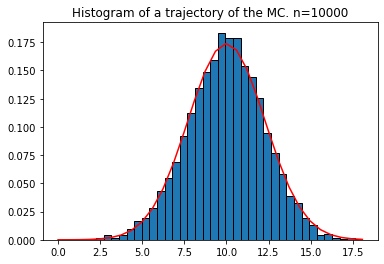
\includegraphics[scale=0.5]{exercise2}

\end{center}
\end{exercise}
%
\begin{exercise}
\label{exo:invar:two}
Consider a Markov chain whose state space $\Xset=(0,1)$ is the open
unit interval. If the chain is at $x$, it picks one of the two intervals
$(0,\ x)$ or $(x,\ 1)$ with equal probability $1/2$, and then moves
to a point $y$ which is uniformly distributed in the chosen interval.
\begin{enumerate}
\item Show that this Markov chain has a transition density wrt the Lebesgue
measure on the interval $(0,1)$, which is given by
\[
k(x,y)=\frac{1}{2}\frac{1}{x}\1_{(0,x)}(y)+\frac{1}{2}\frac{1}{1-x}\1_{(x,1)}(y)
\]

\item Show that this Markov chain can be equivalently represented as an
iterated random sequence.
\[
X_{t}=\epsilon_{t}\left[X_{t-1}U_{t}\right]+(1-\epsilon_{t})\left[X_{t-1}+U_{t}(1-X_{t-1})\right]
\]
 where $\seq{U_{n}}{n\in\nset}$ and $\seq{\epsilon_{n}}{n\in\nset}$
are iid random variables whose distribution should be given.
\item Assuming that the stationary distribution has a density $p$ wrt the
Lebesgue measure show that
\[
p(y)=\frac{1}{2}\int_{y}^{1}\frac{p(x)}{x}\rmd x+\frac{1}{2}\int_{0}^{y}\frac{p(x)}{1-x}\rmd x
\]

\item Deduce that
\[
\int_{0}^{z}p(y)\rmd y=2C\,\mathrm{arcsin}(\sqrt{z})
\]
for some constant $C$.
\item Conclude that $C=1/\pi$.
\end{enumerate}
Details of the numerics are given in the Jupyter Notebook.

\begin{center}

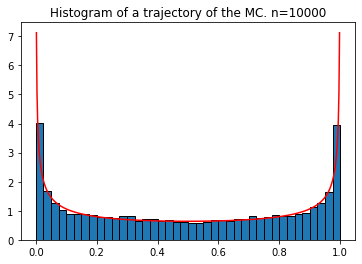
\includegraphics[scale=0.5]{exercise3}

\end{center}
\end{exercise}
%
\begin{exercise}\label{exo:gibbs}
Let $\pi(\rmd x\rmd y)=\pi(x,y)\lambda_X(\rmd x) \lambda_Y(\rmd y)$ be probability measure on $(\Xset \times \Yset, \Xsigma \otimes \Ysigma)$ where  $\lambda_X$ (resp. $\lambda_Y$) is $\sigma$-finite measure on $(\Xset,\Xsigma)$ (resp. $(\Yset,\Ysigma)$). Define $\pi(y|x)=\frac{\pi(x,y)}{\pi(x)}$ whenever $\pi(x)\neq 0$.

Define: $P( (x,y),\rmd x'\rmd y')= \delta_x(\rmd x') \pi(y'|x) \lambda_Y(\rmd y')$. Show that $P$ is a $\pi$-reversible Markov kernel on  $(\Xset \times \Yset) \times (\Xsigma \otimes \Ysigma)$.
\end{exercise}

\begin{exercise}\label{exo:detailed}
In a MH algorithm, we want to find an acceptance probability $\alpha(x,y)=f\lr{\frac{\pi(y)q(y,x)}{\pi(x) q(x,y)}}$
\begin{enumerate}
\item Show that the detailed balance condition is satisfied if and only if for all $u\geq 0$, $f(u)=uf(1/u)$.
\item Show that it is sufficient to check that for all $u\in (0,1)$, $f(u)=uf(1/u)$.
\item Find all the functions $f$ sucht that the detailed balance condition is satisfied with $\alpha(x,y)=f\lr{\frac{\pi(y)q(y,x)}{\pi(x) q(x,y)}}$.
\end{enumerate}
\end{exercise}



%
\begin{exercise}
Let $P$ be a Markov kernel with invariant probability measure $\pi$.
Let $A\in\Xsigma$ such that $\pi(A)=1$. Show that there exists $B\subset A$
such that $P(x,B)=1$ for all $x\in B$ (i.e. such set $B$ is said
to be \emph{absorbing} in the sense that starting from any point in
$B$, the Markov chain stays in $B$ forever with probability one).
\end{exercise}
%

\begin{exercise} \label{exo:arp}
Let $(X_t)$ be the AR(p) process defined by: $X_t=\sum_{i=1}^{p} a_i X_{t-i}+\sigma \epsilon_t$ for all $t\geq i$,  where $\epsilon_i \iid \gauss(0,1)$ and $\sigma>0$.

Define $Y_t=\begin{pmatrix}
X_t\\
\ldots\\
X_{t-p+1}
\end{pmatrix}$ and show that $(Y_t)$ is a Markov chain. Give the expression of the associated Markov kernel. Show that it admits at most one invariant probability measure.
\end{exercise}

\begin{exercise}
Let $P$ be a Markov kernel on $\Xset\times\Xsigma$, admitting an
invariant probability measure $\pi$. We assume that there exist two
measurable positive functions $V$ and $f$ and a constant $K$ such
that
\[
PV+f\leq V+K. 
\]
Show that $\pi(f)<\infty$.
\end{exercise}

\begin{exercise} \label{exo:birk}
In this exercise, we prove \autoref{thm:birk:dynam}.
Set $S_n=\sum_{k=0}^{n-1}h\circ T^{k}$, $L_n=\inf\set{S_k}{k\in[1:n]}$ and $A=\lrcb{\inf_{n\in\nset^*}L_n=-\infty}$.
We first assume that $\PE[h]>0$.
\begin{enumerate}
\item Show that $L_n \geq h+\inf(0,L_n\circ T)$.
\item Deduce that
$$
\PE[\indi{A} h] \leq \PE[\indi{A} (L_n)^+]
$$
\item Deduce $\PP(A)=0$.
\item Prove The Birkhoff theorem (\autoref{thm:birk:dynam}).
\end{enumerate}
\end{exercise}

%
\begin{exercise}\label{exo:LLN:Aone:Atwo}
Assume that \ref{assum:Aone} and \ref{assum:Atwo}\ hold for some measurable function $V\geq 1$. We want to prove that: for all initial
distributions $\nu\in\meas 1(\Xset)$ and all $f\in\funcset{}(\Xset)$
such that $\pi(|f|)=\int_{\Xset}\pi(\rmd x)|f(x)|<\infty$,
\begin{equation}
\lim_{n\to\infty}n^{-1}\sum_{k=0}^{n-1}f(X_{k})=\pi(f)\,,\quad\PP_{\nu}-a.s\label{eq:LLN:gener}
\end{equation}
\begin{enumerate}
\item Prove the result by combining Corollary~\ref{cor:ergod} and \autoref{thm:ergo:geom} with some results in Chapter 3 (give the exact references of the results that you pick from Chapter 3)
\end{enumerate}
\end{exercise}

\begin{exercise} \label{exo:discretiz:Hamilton}
Consider the following discretization of the Hamiltonian dynamics.
\begin{align}
p^{k+1}&=p^k-(h) \nabla U(q^k) \nonumber\\
q^{k+1}&=q^k+h p^{k+1} \label{eq:leap:update}
\end{align}
\begin{enumerate}
\item Is it volume-preserving?
\item Can we to the flip operator trick to obtain an involution?
\end{enumerate}
\end{exercise}

%\chapter*{Index }

\printindex
\end{document}
